\section{舞踊分類ネットワーク}

\subsection{モデル概要}
今回のモデルでは入力された動画を[優美なダンス,普通のダンス,その他の動作]に分類した.
モデルから直接に入力動画のどこが優美か特定させることは困難だと考え,まずは動画をクラス分類することを
考えた.研究の初期段階では[優美なダンス,その他の動作]の二値分類を学習させたが,主に
優美ではないダンスの精度が著しく低迷しており,そのほとんどが優美に分類された.

ここから考えられることとして,[優美なダンス,その他の動作]と分類しようとしていたところが,
[リズミカルな動作,その他の動作]と分類されたことが考えられた.
ここで優美なダンスと普通のダンスを「リズミカルな動作」という大きな括りの中に属していることを考えると
優美なダンスとその他の動作のみで普通のダンスを区別することは困難に思われた.
そこで優美なダンスと普通のダンスを区別してクラス分けすることで精度が飛躍的に上昇した.

モデルを簡単なフローチャートで表現すると図\ref{easy_chart}のようになる.
\begin{enumerate}
  \item 動画を特殊な二値化手法で編集する.詳細は2.2節で述べる.
  \item 二値データと,それに対応するピクセル番号を畳み込む.
  \item 二つのデータを足し合わせる.
  \item Transformer Encoderに通した後,全結合し,Softmaxにかける.
\end{enumerate}
のようにモデル内で計算し,クラス分けを実現した.

最適化アルゴリズムにAdam\cite{adam},損失関数に交差エントロピー誤差(\ref{entropy})を使用した.
\begin{equation}
  H(t, p) = -\sum_{i}t_i\log p_i
  \label{entropy}
\end{equation}

入力されるデータは,目標となる教師データtとネットワークから推論されたデータpである.
それぞれの配列長はiとする.それらを上記の式に当てはめ,配列長iまで総和を取ることで
推論がどれだけ目標に近いか1以下の数値で計算し,その値を元にAdamが各層の値を更新する.
\clearpage

\begin{figure}[t]
  \begin{center}
    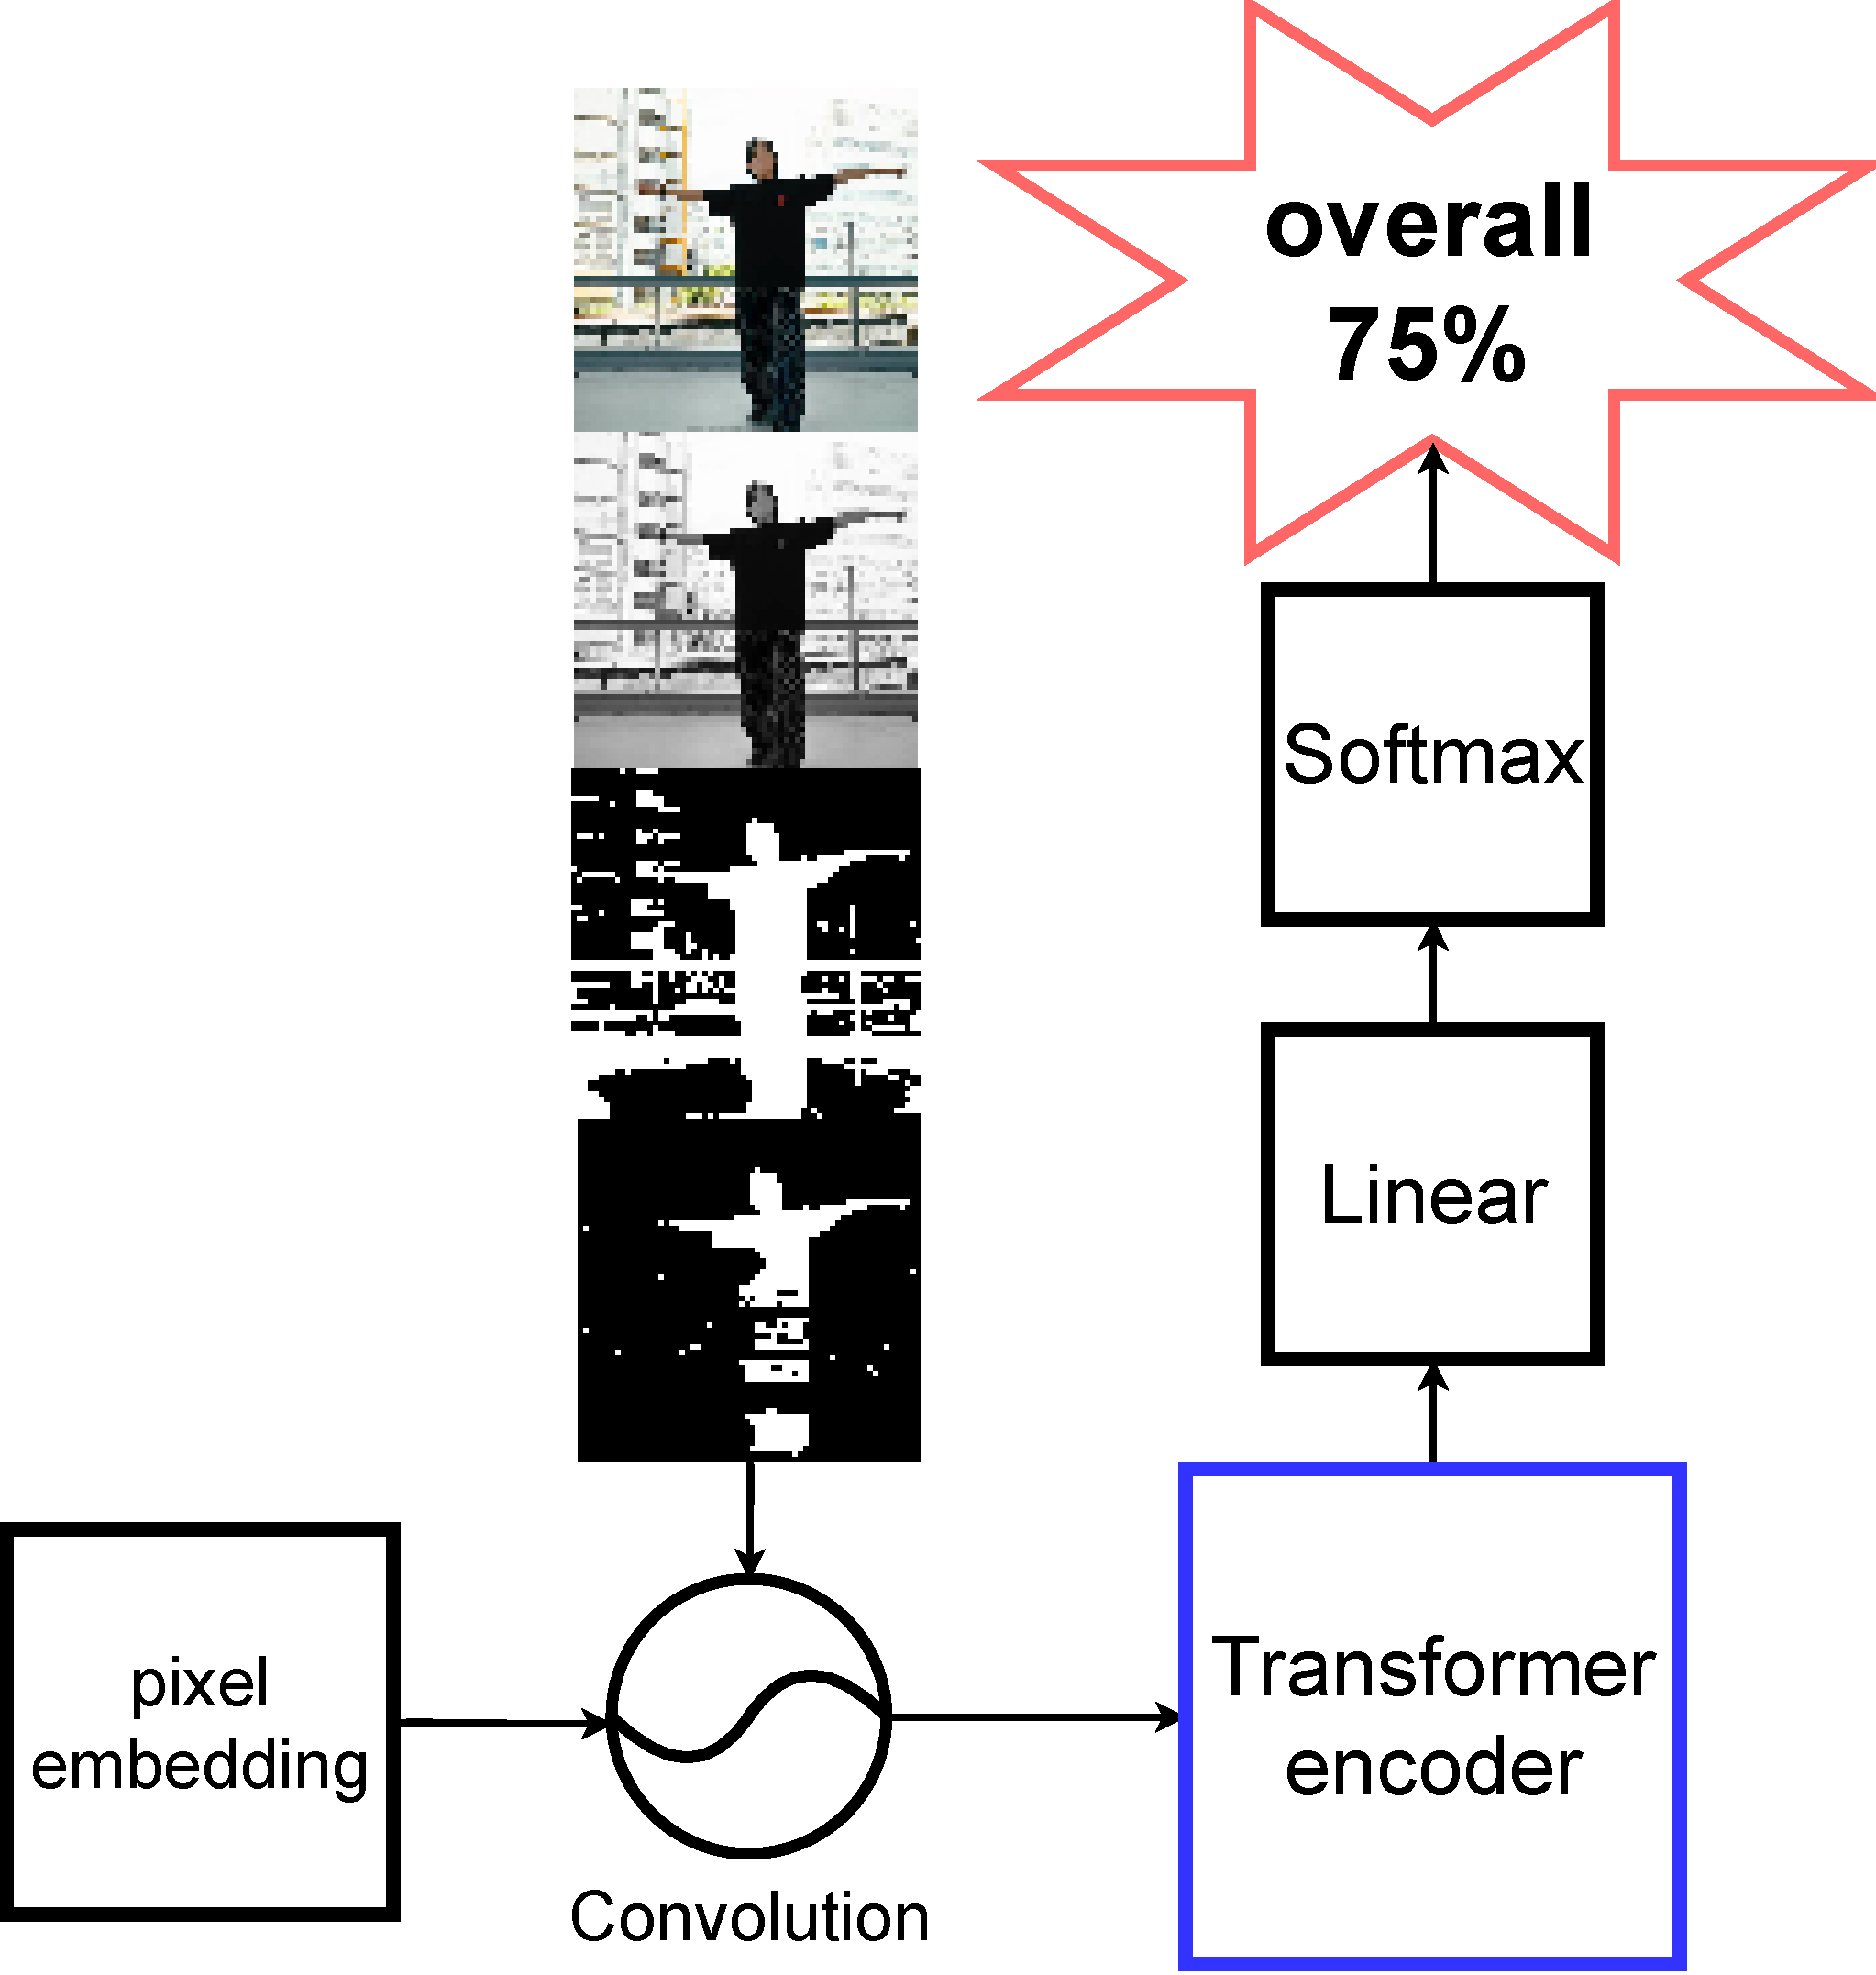
\includegraphics[width=80mm]{images/chart/easy_chart.pdf}
  \end{center}
  \caption{モデル概要}
  \label{easy_chart}
\end{figure}

\subsection{使用する動画データ}
動画は表\ref{video_data}を使用した.優美な動画の選定方法は,youtubeで「優美」「美しい」などの
キーワードで検索し,再生回数の多く,主観で優美であると感じたものを使用した.
国,舞踊の種類が単一であると目的である網羅的な学習を達成できないため,古今東西の舞踊を使用した.
普通のダンスでは同じように「ダンス」「かっこいい」などのキーワードを持ち,再生回数が多いものを使用した.
その他の動作は「ランニング」「体操」など,日常的な動作を使用した.
再生回数が多いものを使用する理由は,その舞踊のエキスパートの動作を
できるだけ使用したかったからである.再生回数が多いということは,それだけ不特定多数から
注目を浴びている,感動を与えていると考えられ,その動作の熟練者である可能性が高いと考えた.
\clearpage

\begin{table}[t]
  \begin{center}
    \begin{tabular}{|c|ccc|cc|} \hline
        & \multicolumn{3}{|c|}{学習用} & \multicolumn{2}{|c|}{推論用} \\ \hline
        &&&&& \\
        & 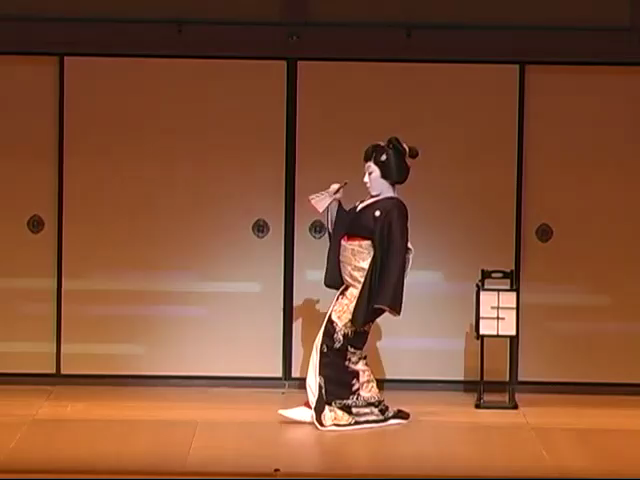
\includegraphics[width=17mm]{images/snaps/japanese_elegant.png}
        & 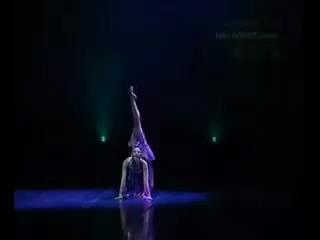
\includegraphics[width=17mm]{images/snaps/chinese_elegant.png}
        & 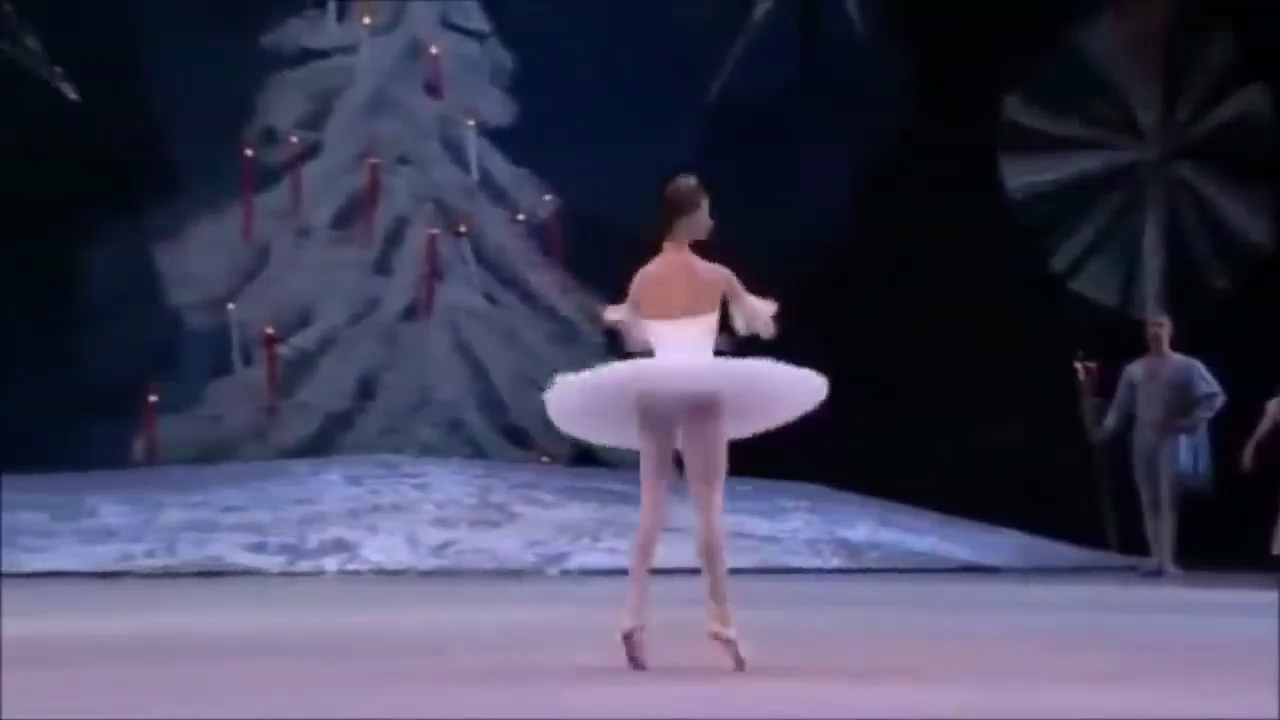
\includegraphics[width=17mm]{images/snaps/ballet_elegant.png}
        & 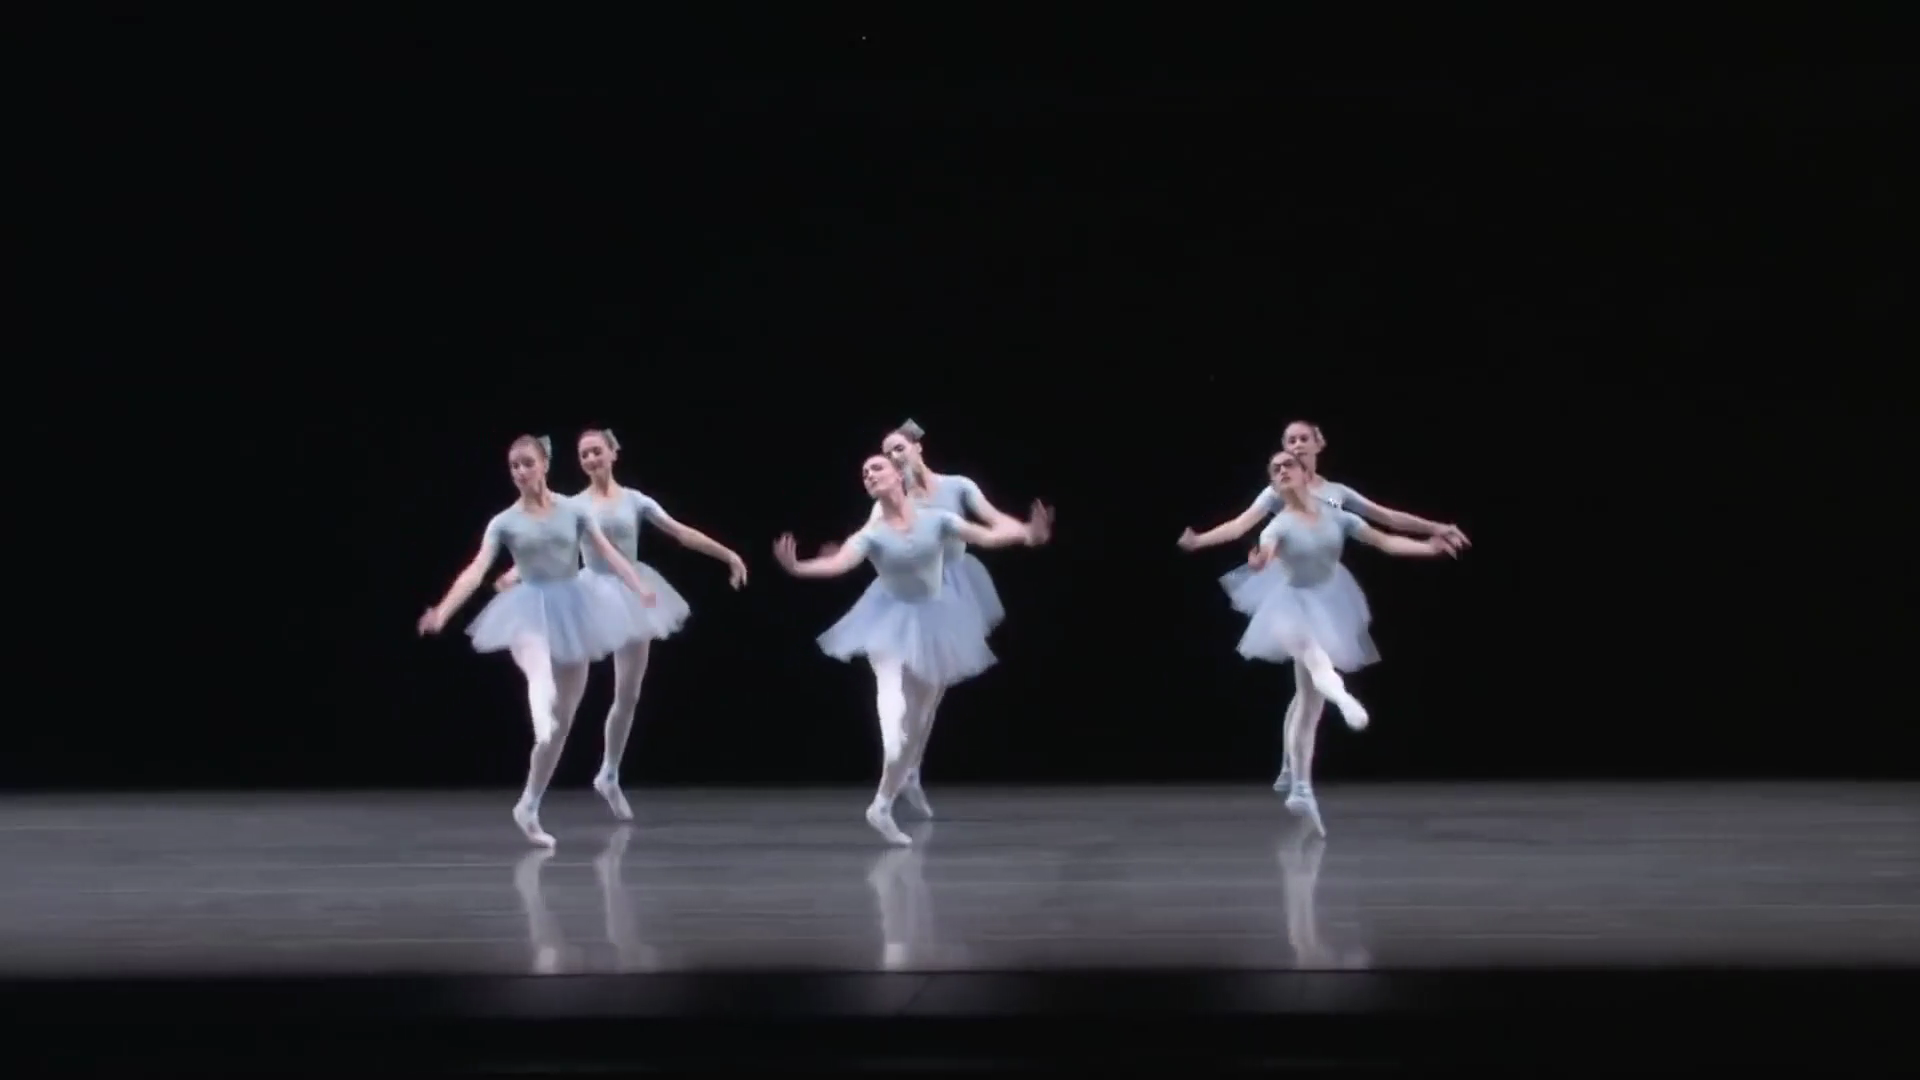
\includegraphics[width=17mm]{images/snaps/ballet_group_elegant.png}
        & 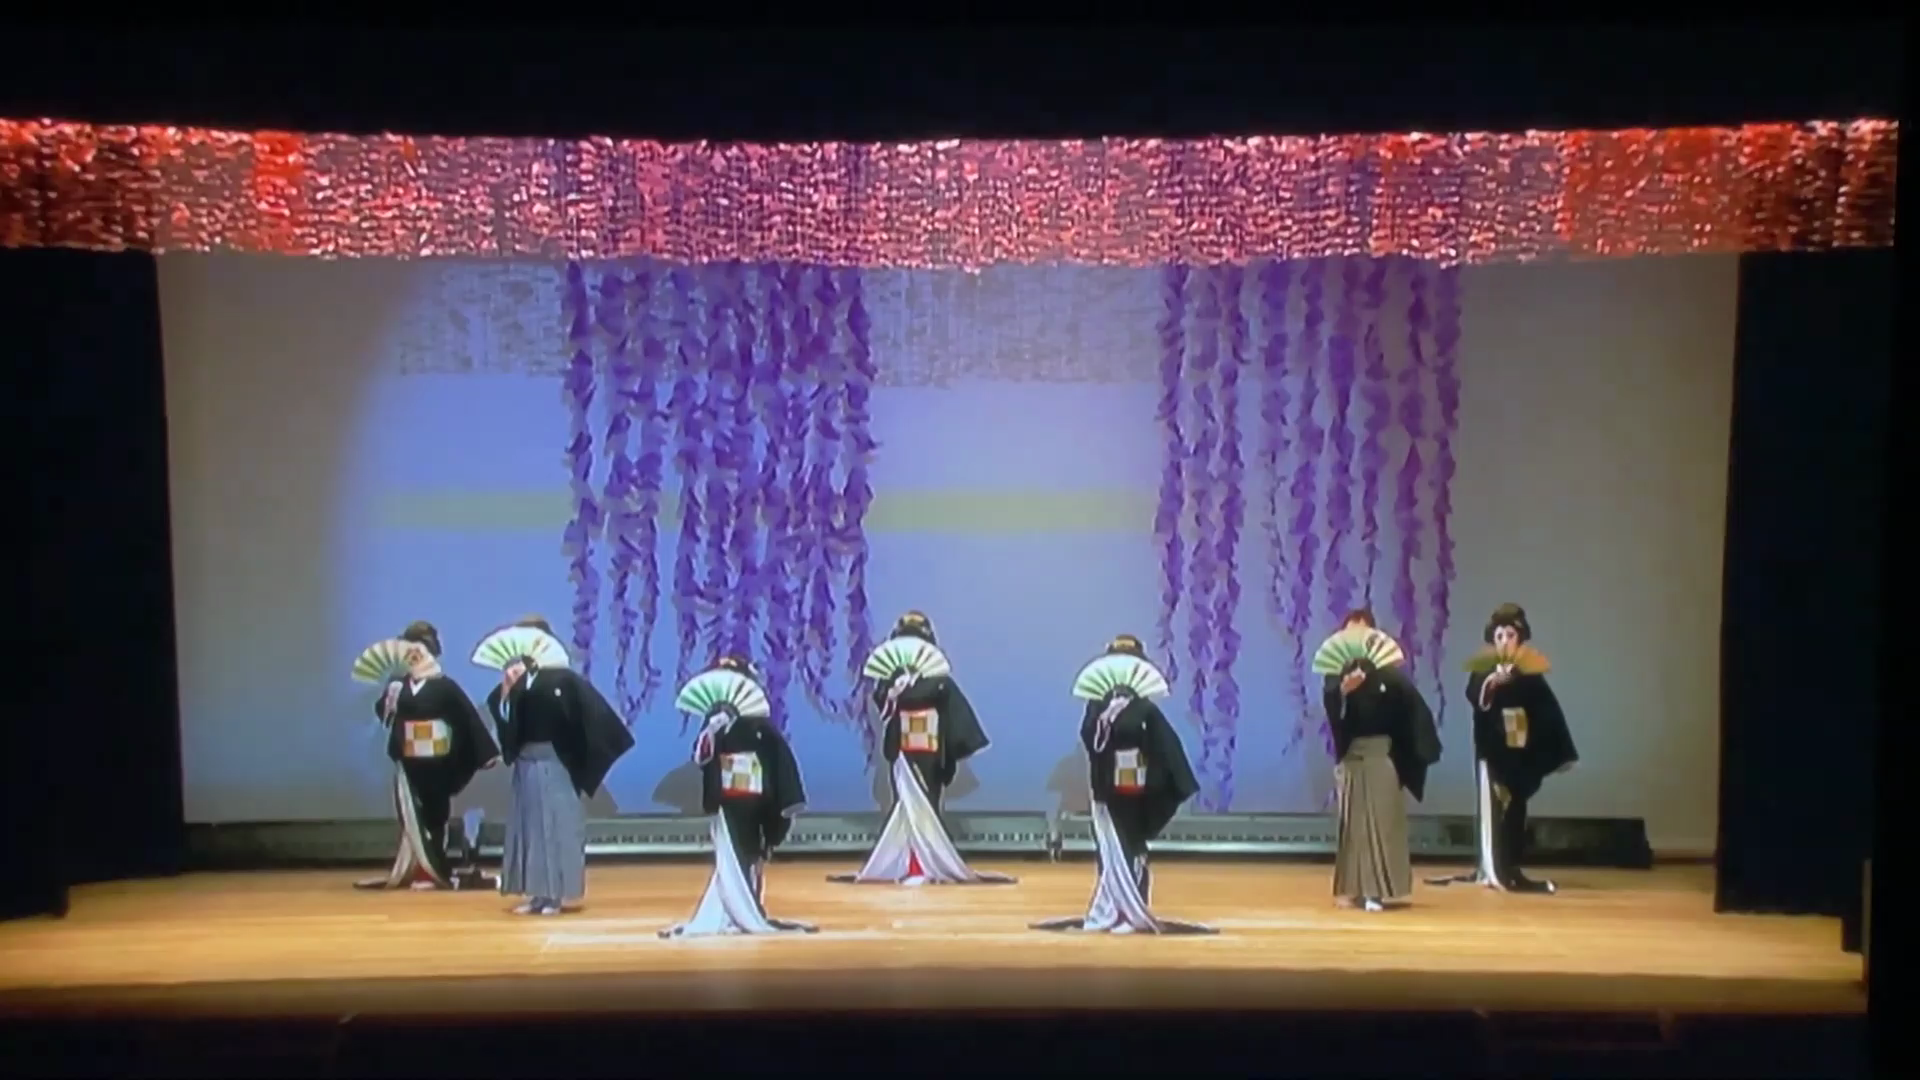
\includegraphics[width=17mm]{images/snaps/japanese_group_elegant.png}
      \\
      優美なダンス & \cite{jpn} & \cite{china} & \cite{ballet} & \cite{balletgroup} & \cite{jpngroup}
      \\
        & 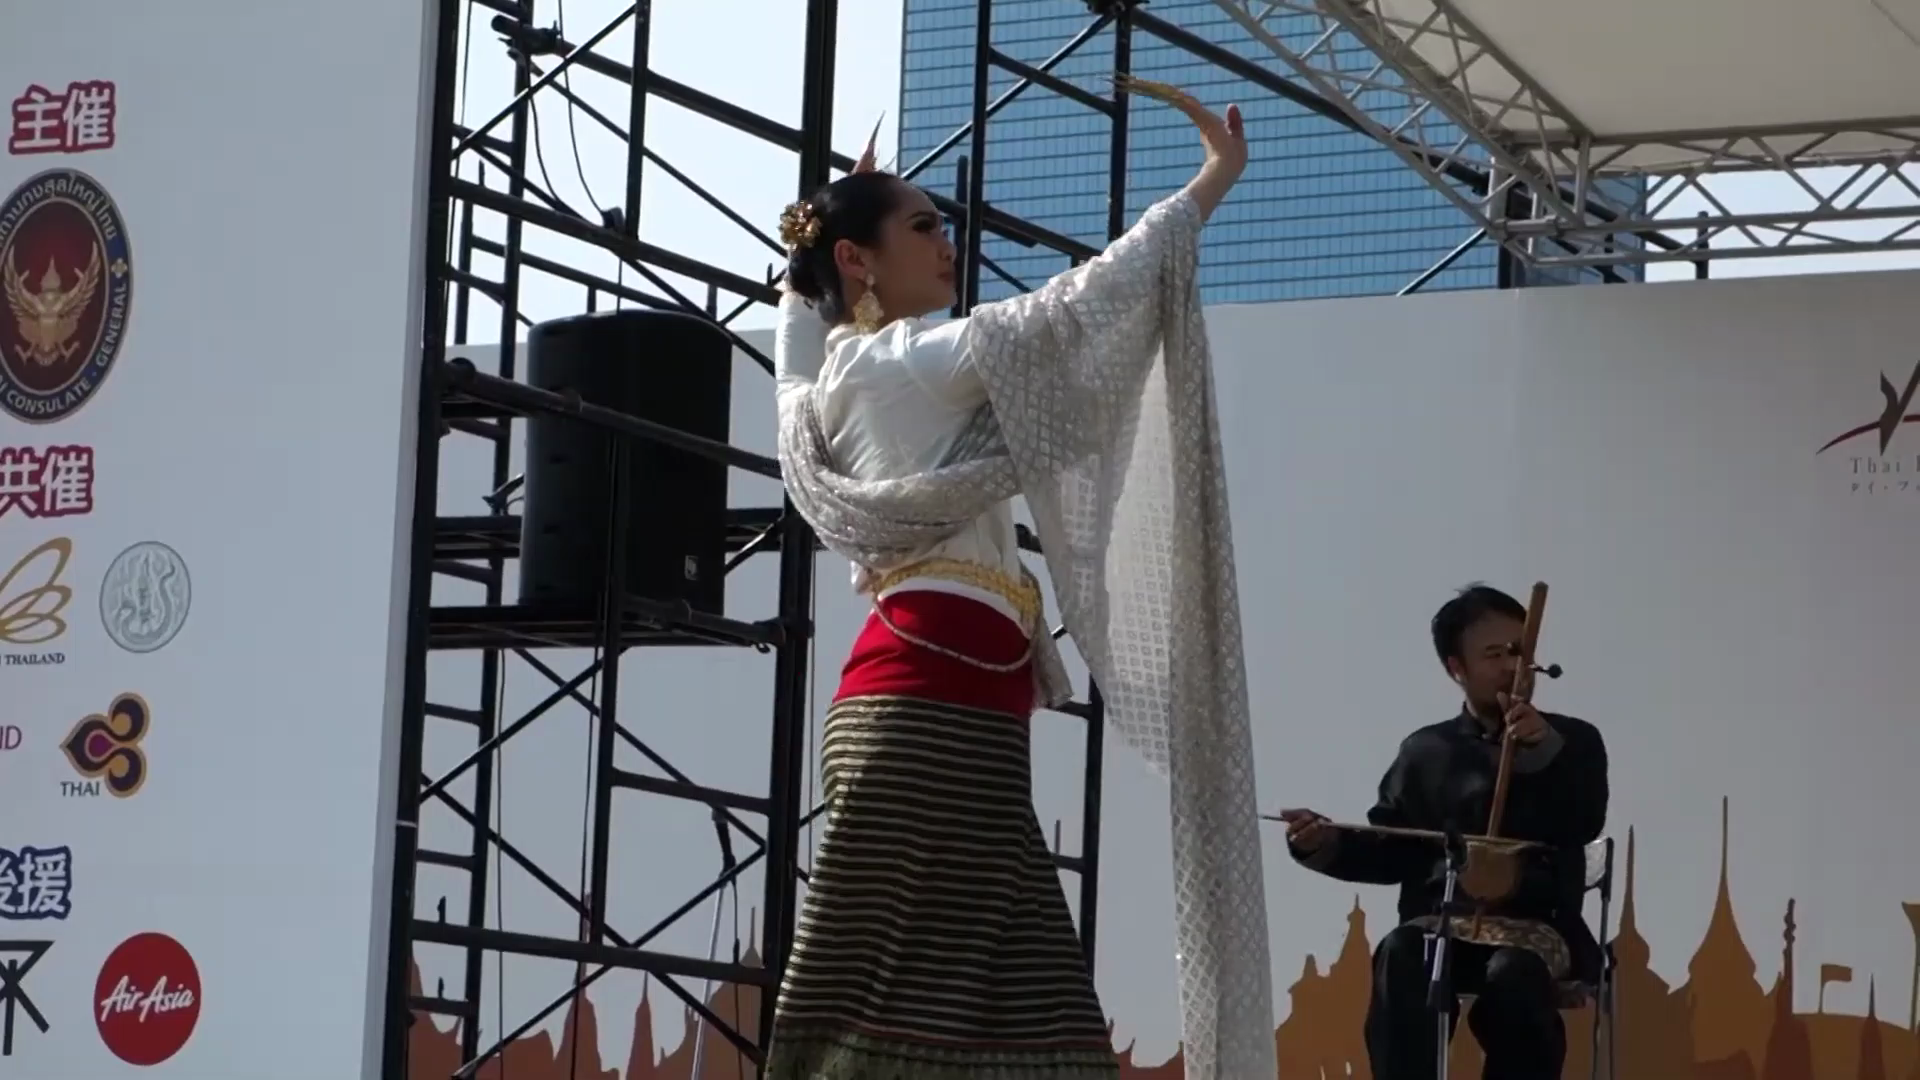
\includegraphics[width=17mm]{images/snaps/thai_elegant.png}
        & 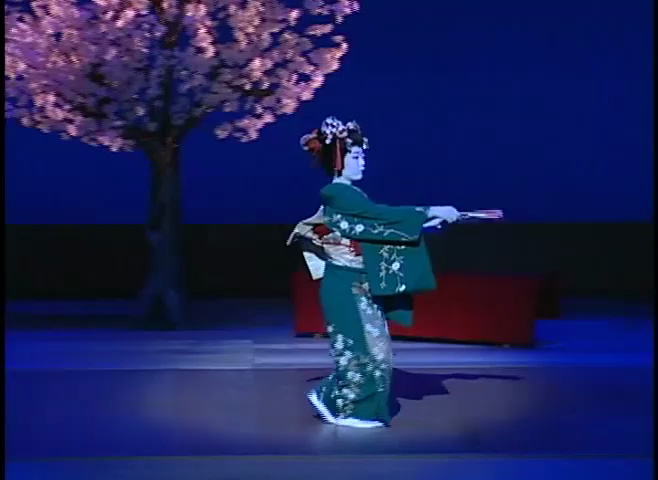
\includegraphics[width=17mm]{images/snaps/japanese2_elegant.png}
        &
        & 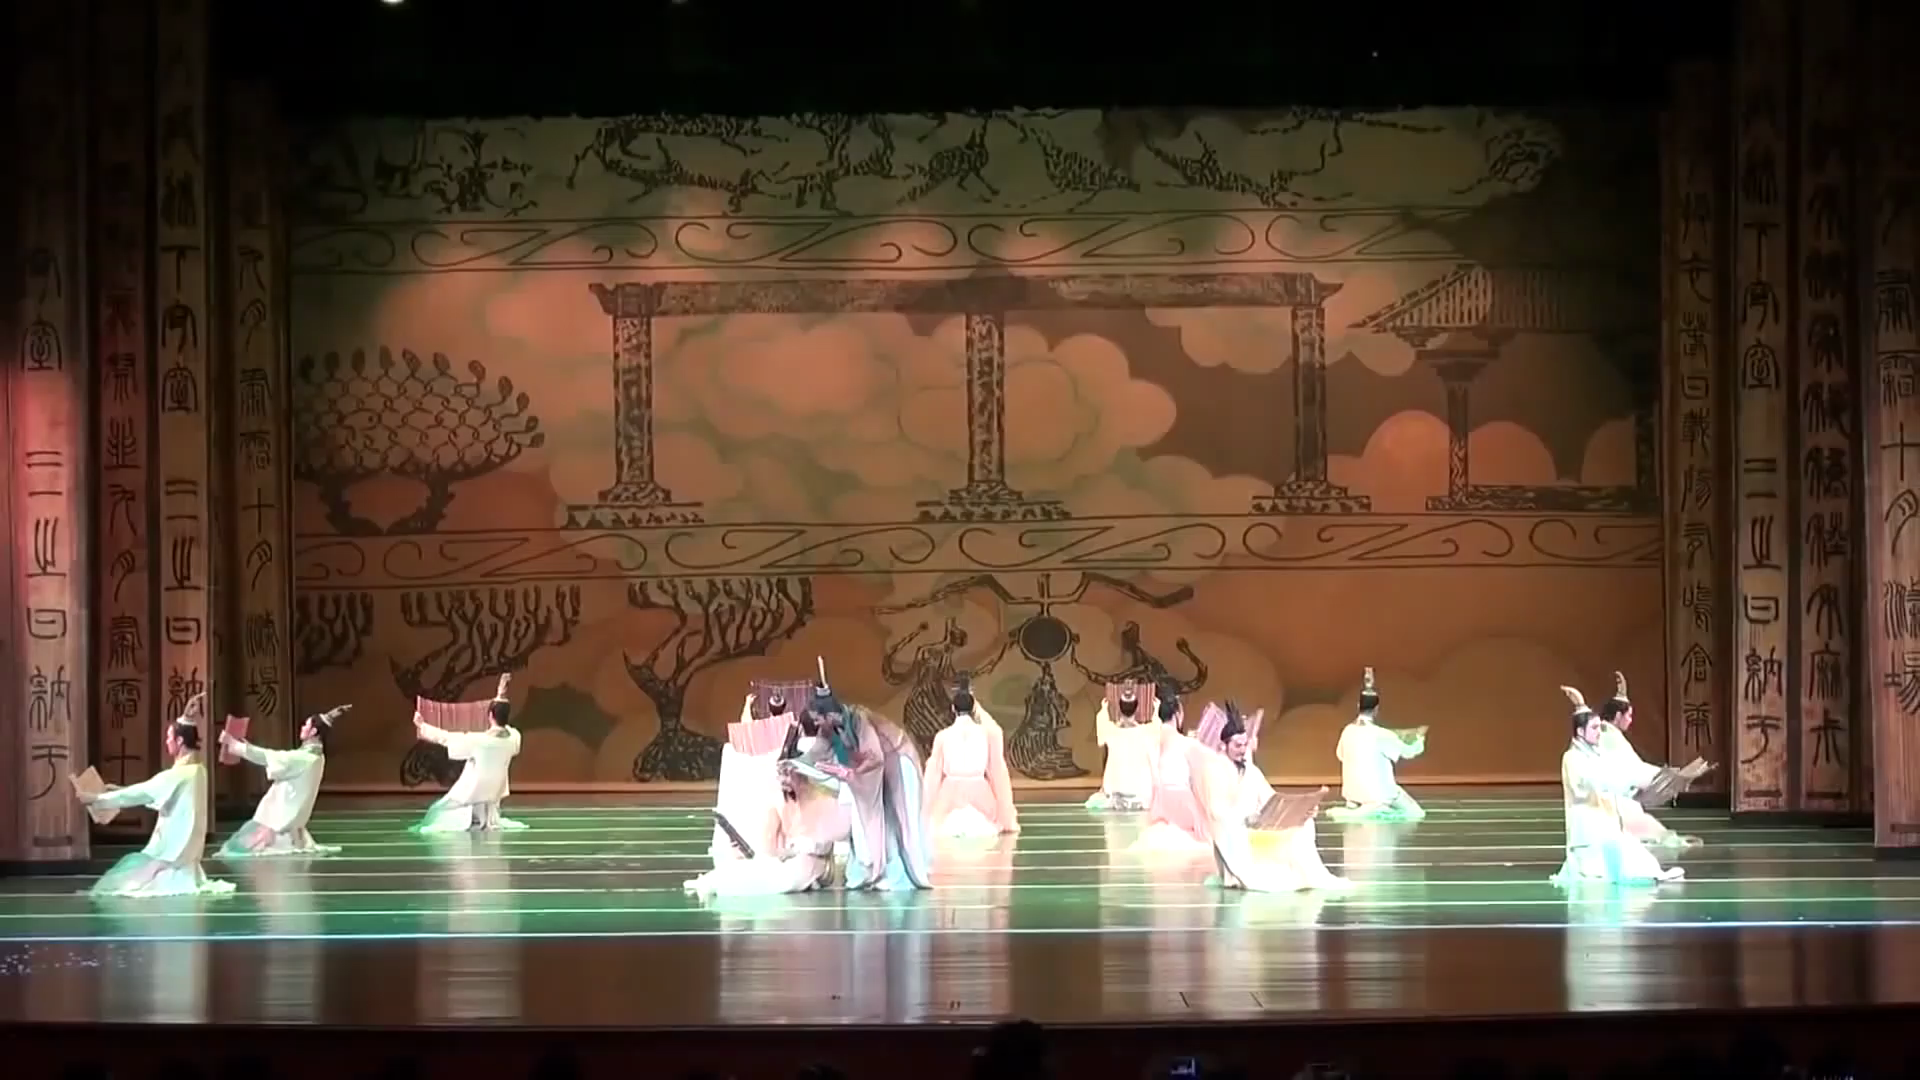
\includegraphics[width=17mm]{images/snaps/chinese_group_elegant.png}
        & 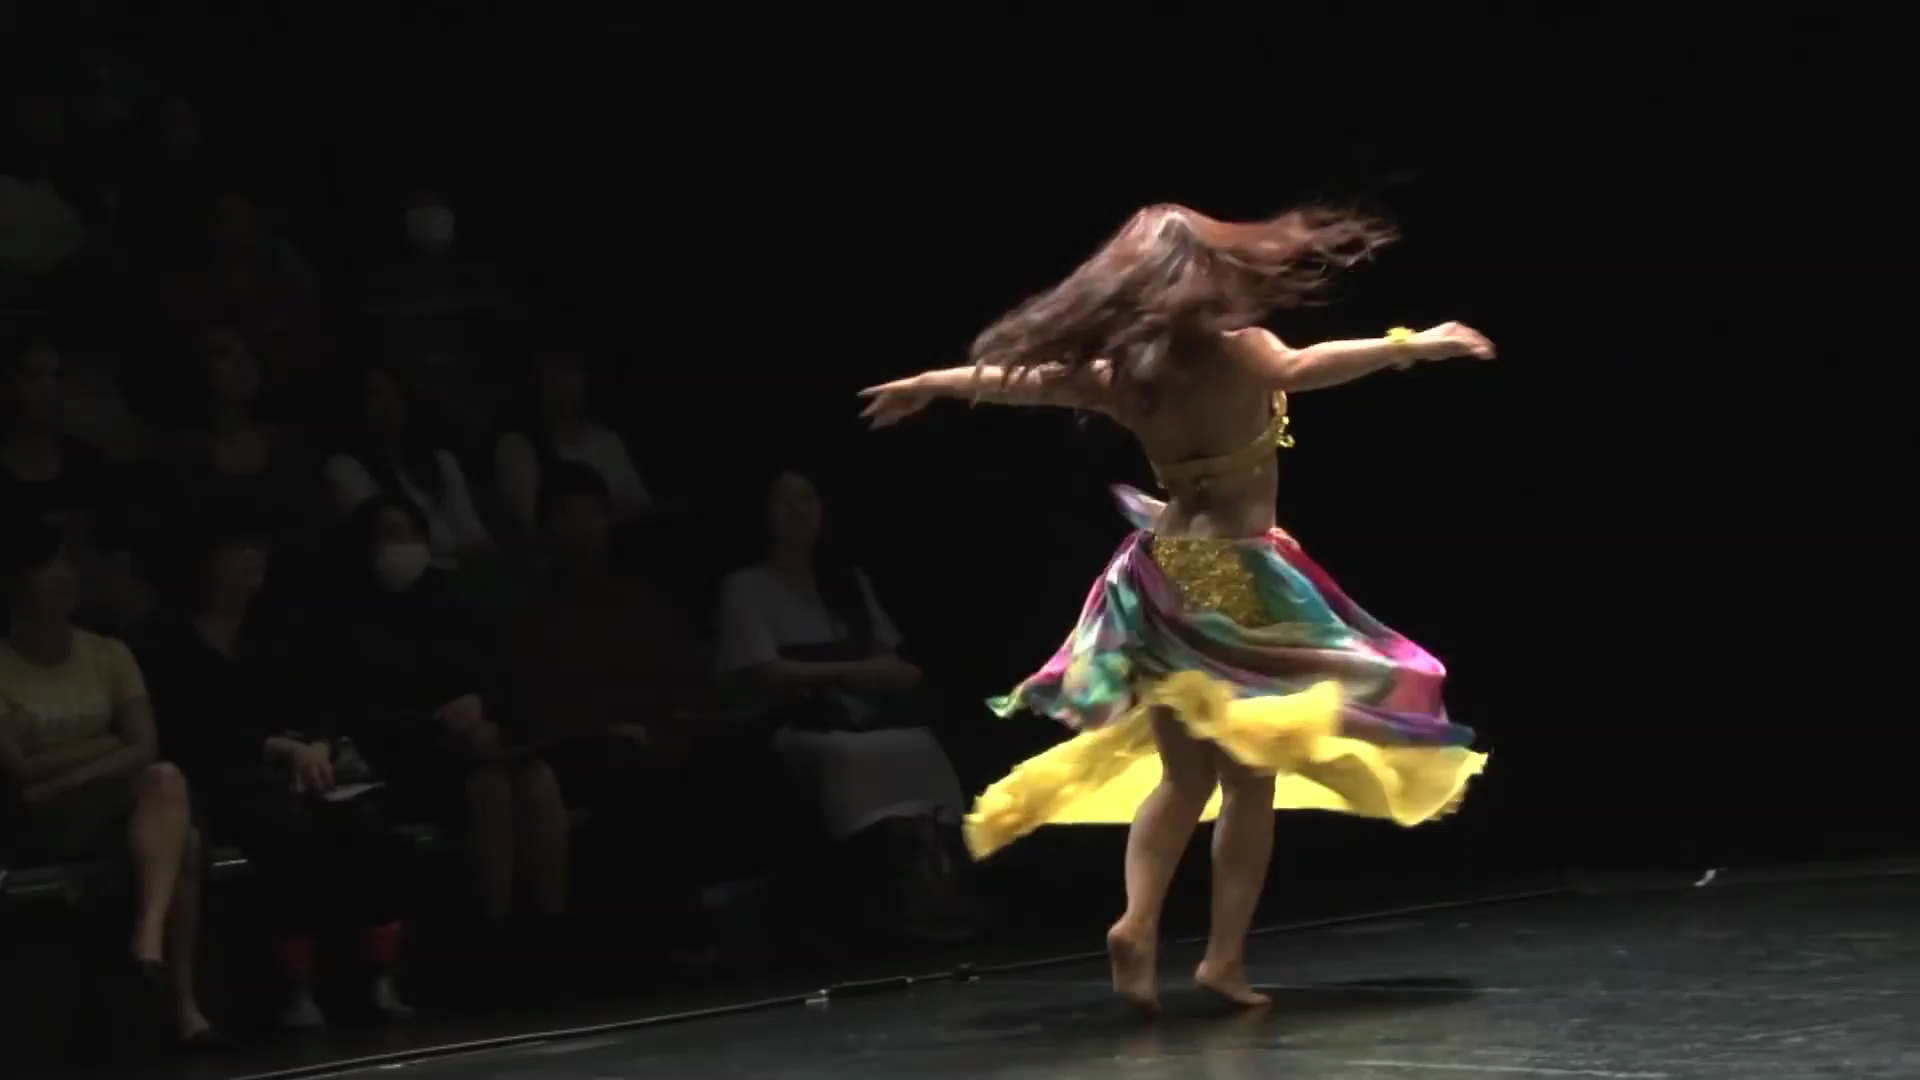
\includegraphics[width=17mm]{images/snaps/belly_elegant.png}
      \\
        & \cite{thai} & \cite{jpn2} & & \cite{chinagroup} & \cite{belly}
      \\ \hline
        &&&&& \\
        & 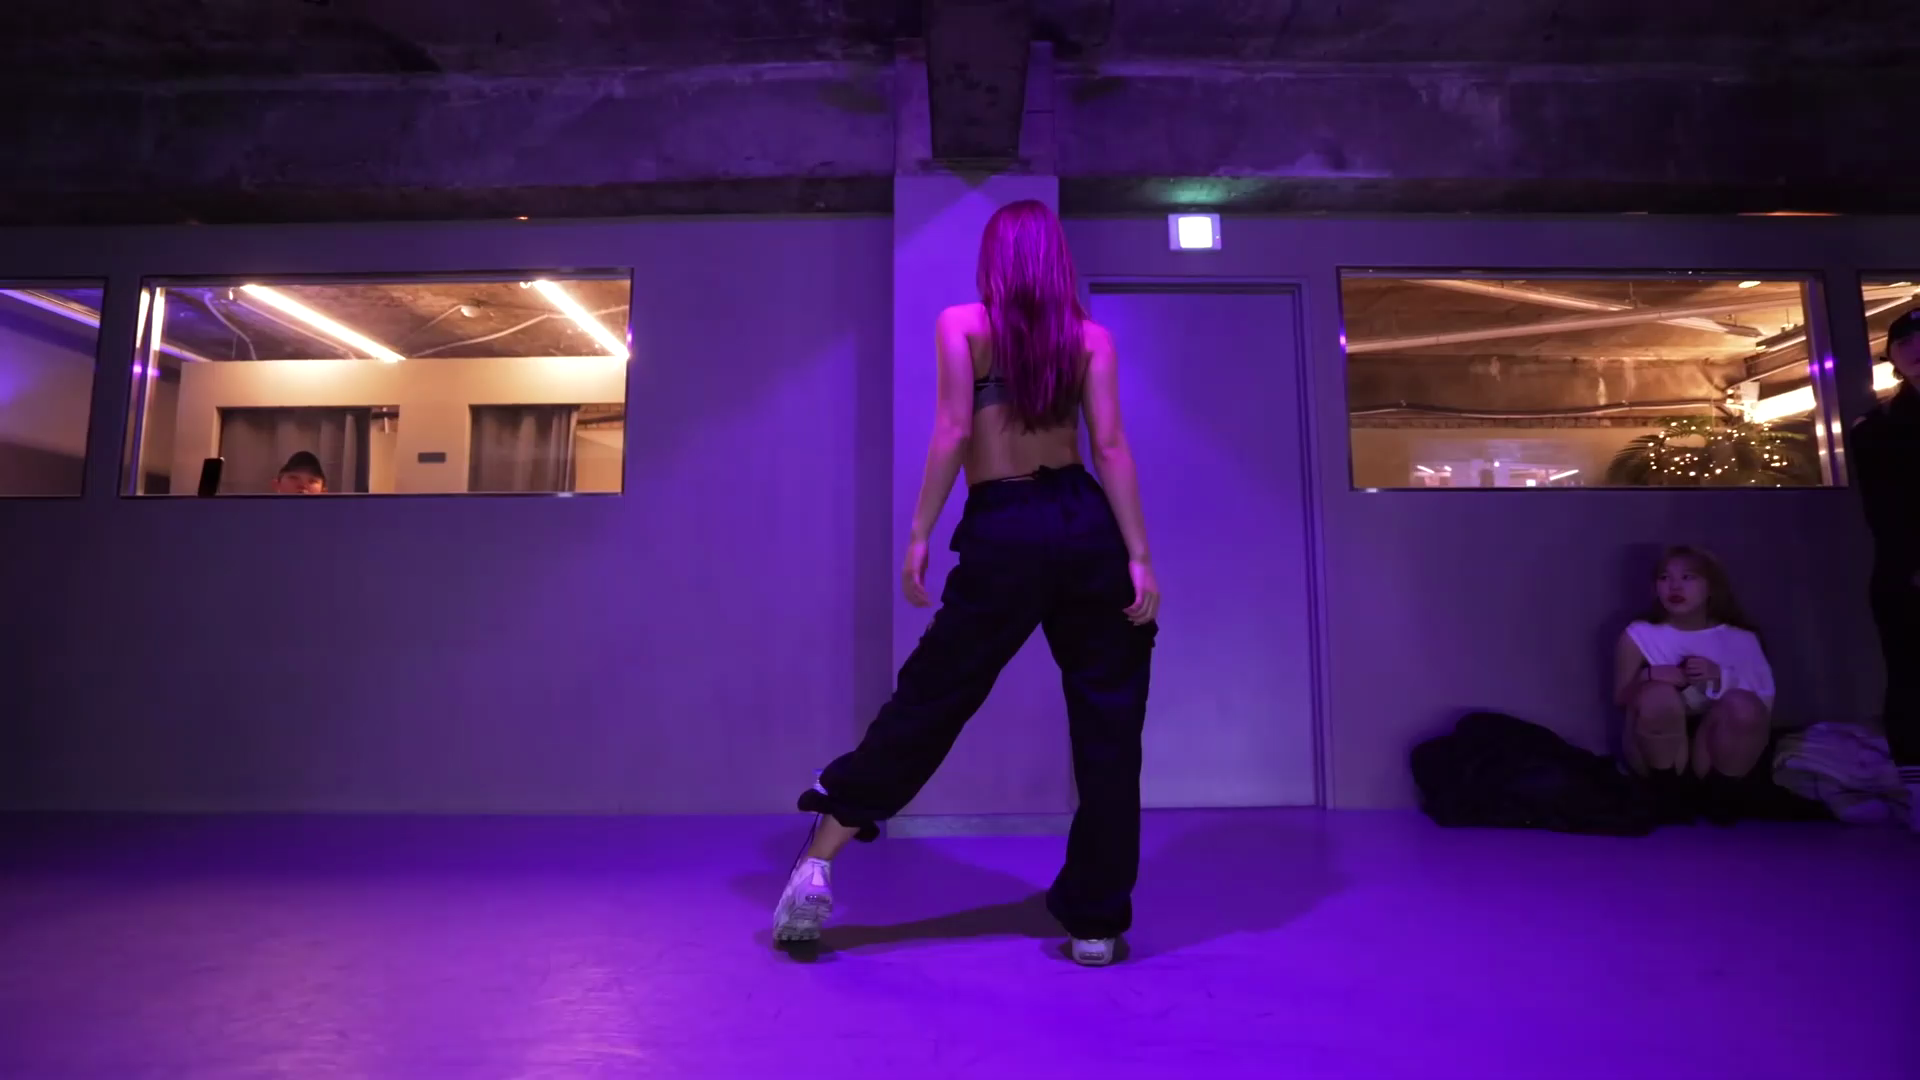
\includegraphics[width=17mm]{images/snaps/ariana_dance.png}
        & 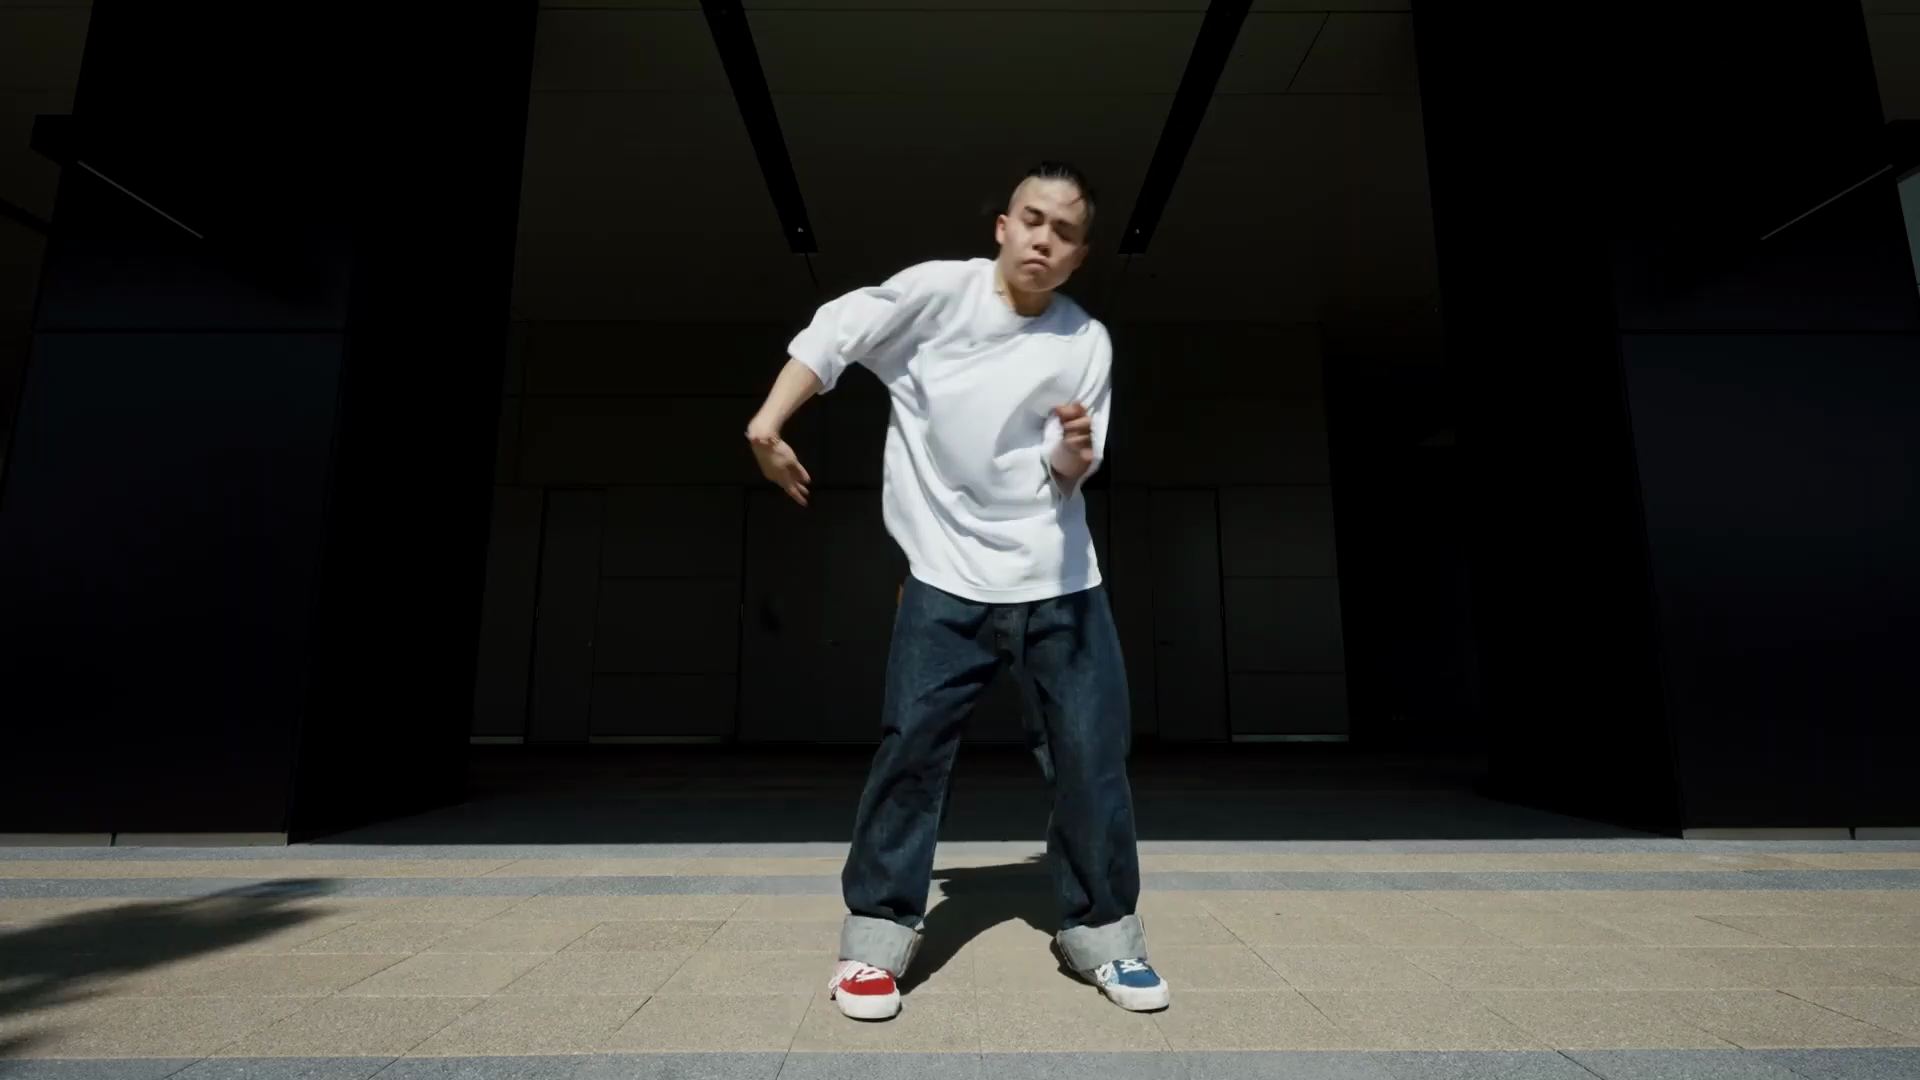
\includegraphics[width=17mm]{images/snaps/kadokawa_dream_dance.png}
        & 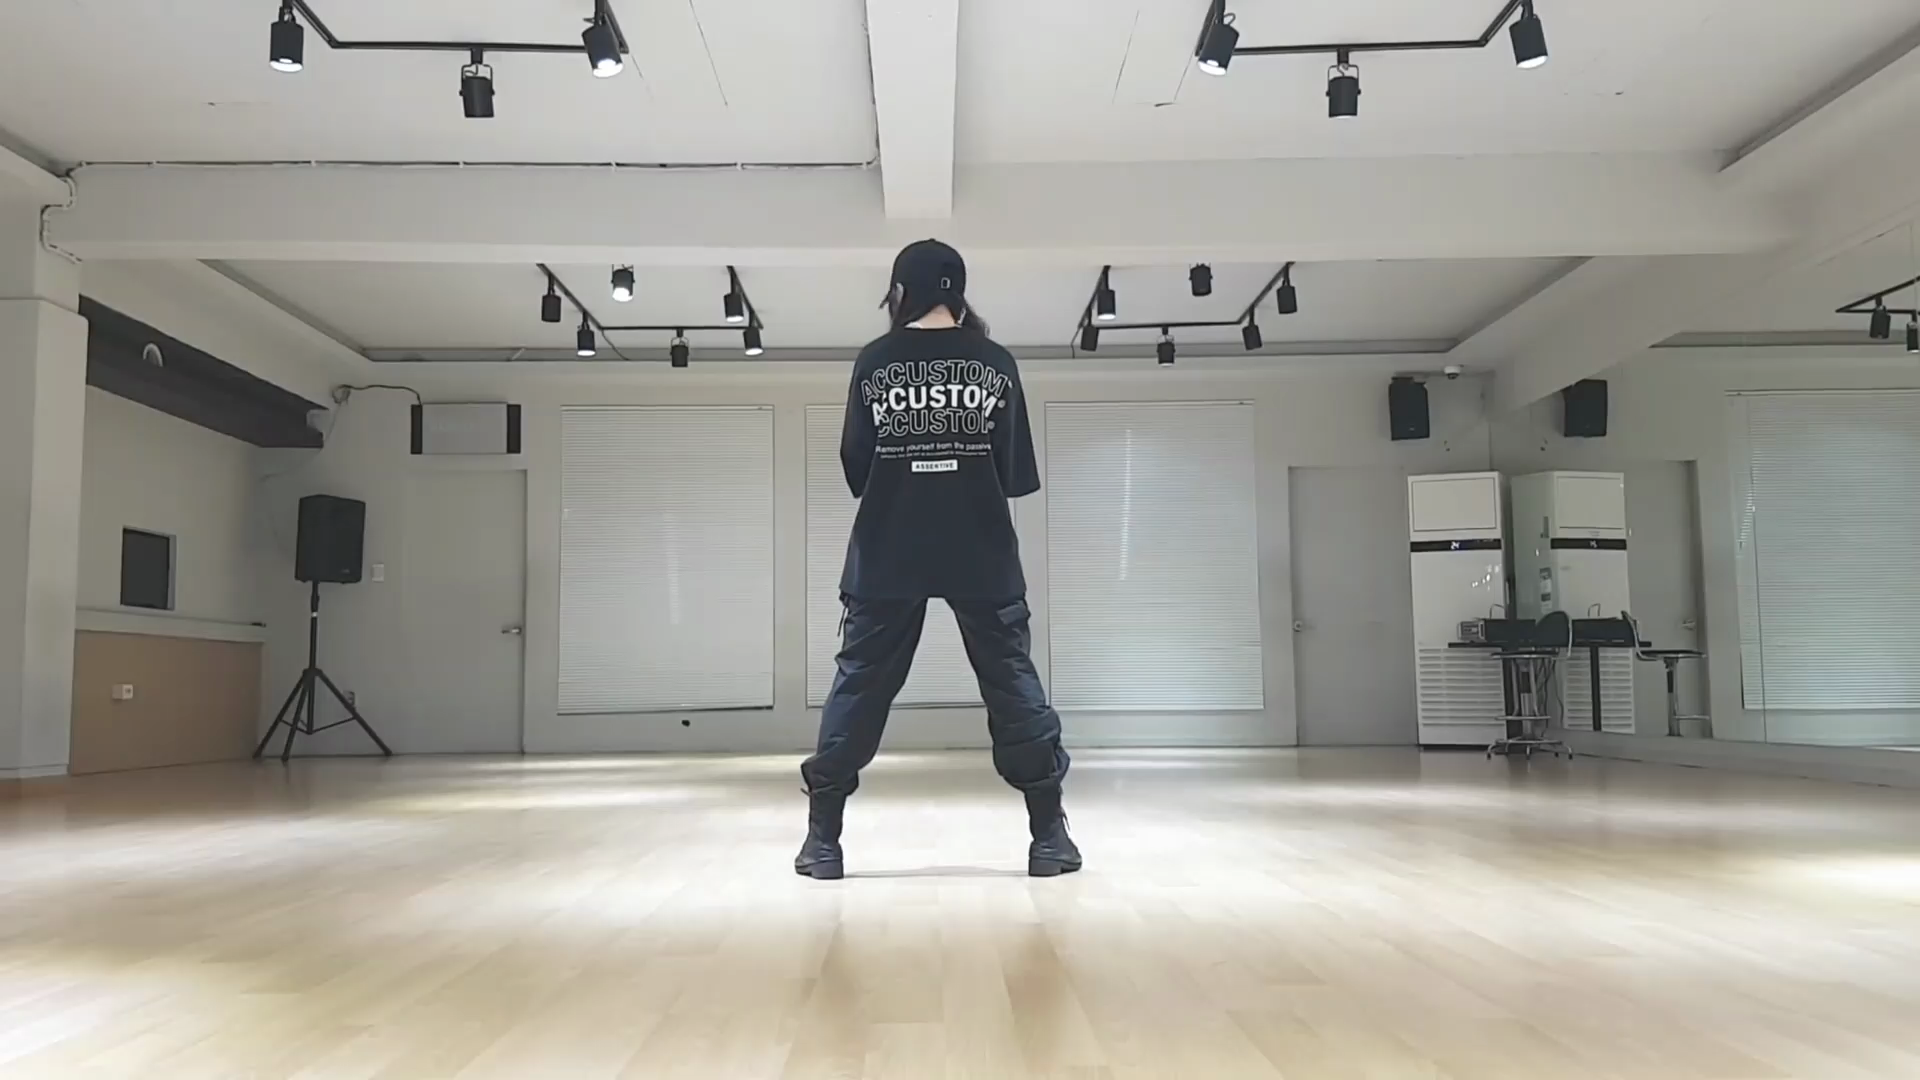
\includegraphics[width=17mm]{images/snaps/bts_dance.png}
        & 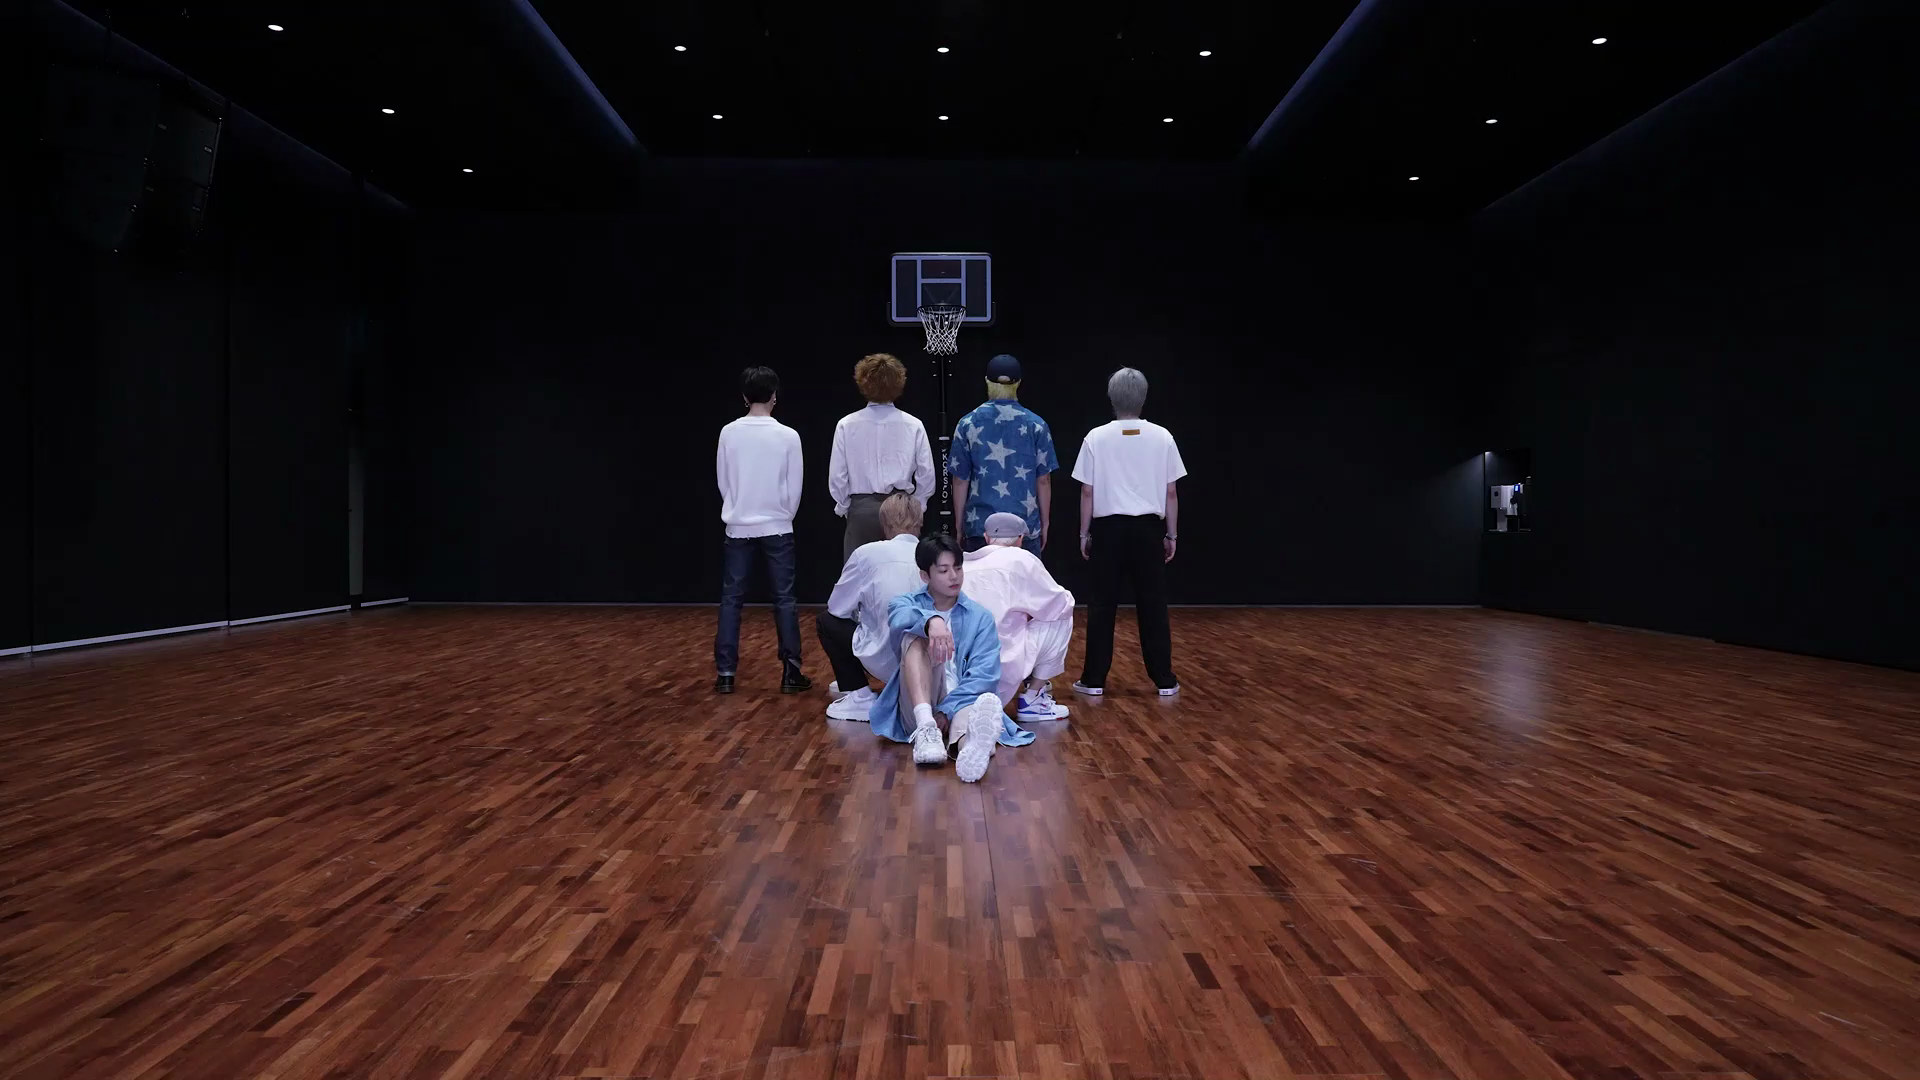
\includegraphics[width=17mm]{images/snaps/bts_group_dance.png}
        & 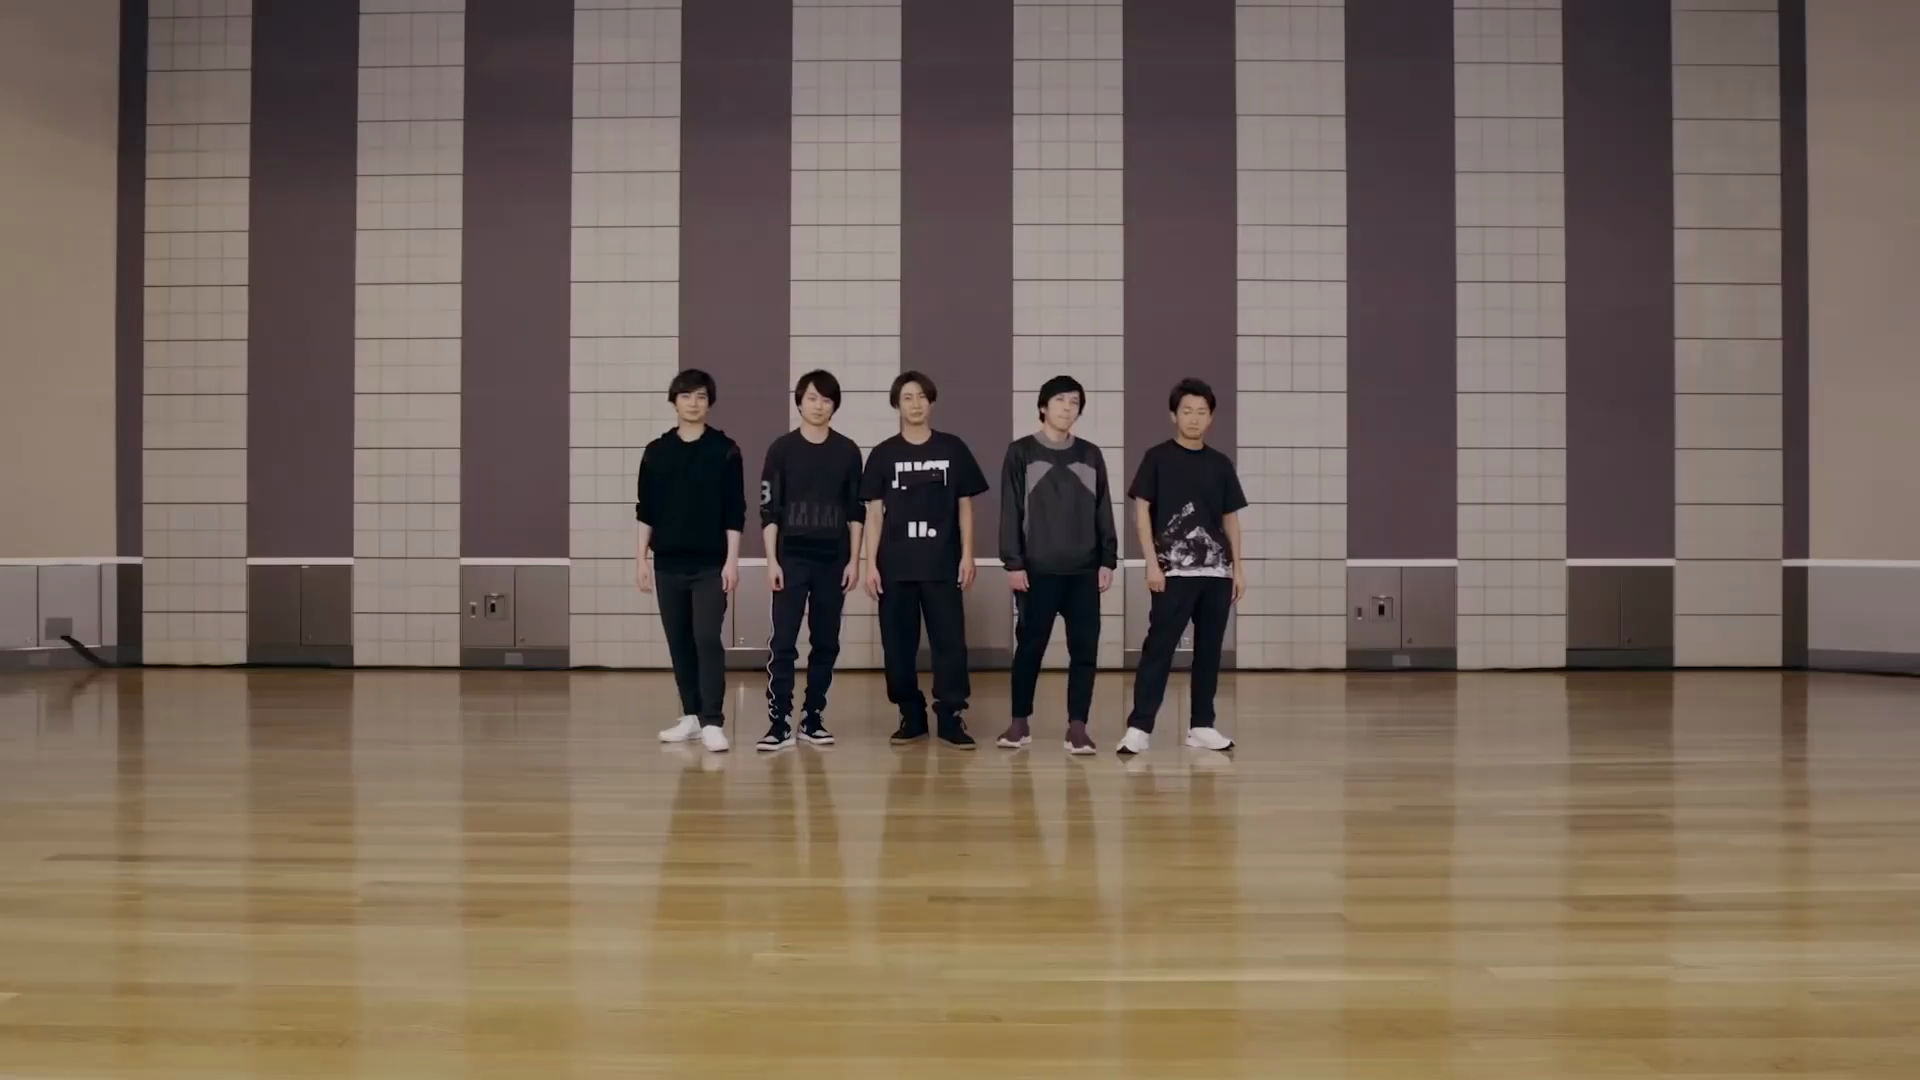
\includegraphics[width=17mm]{images/snaps/arashi_group_dance.png}
      \\
      普通のダンス & \cite{ariana} & \cite{kadokawa} & \cite{bts} & \cite{btsgroup} & \cite{arashi}
      \\
        & 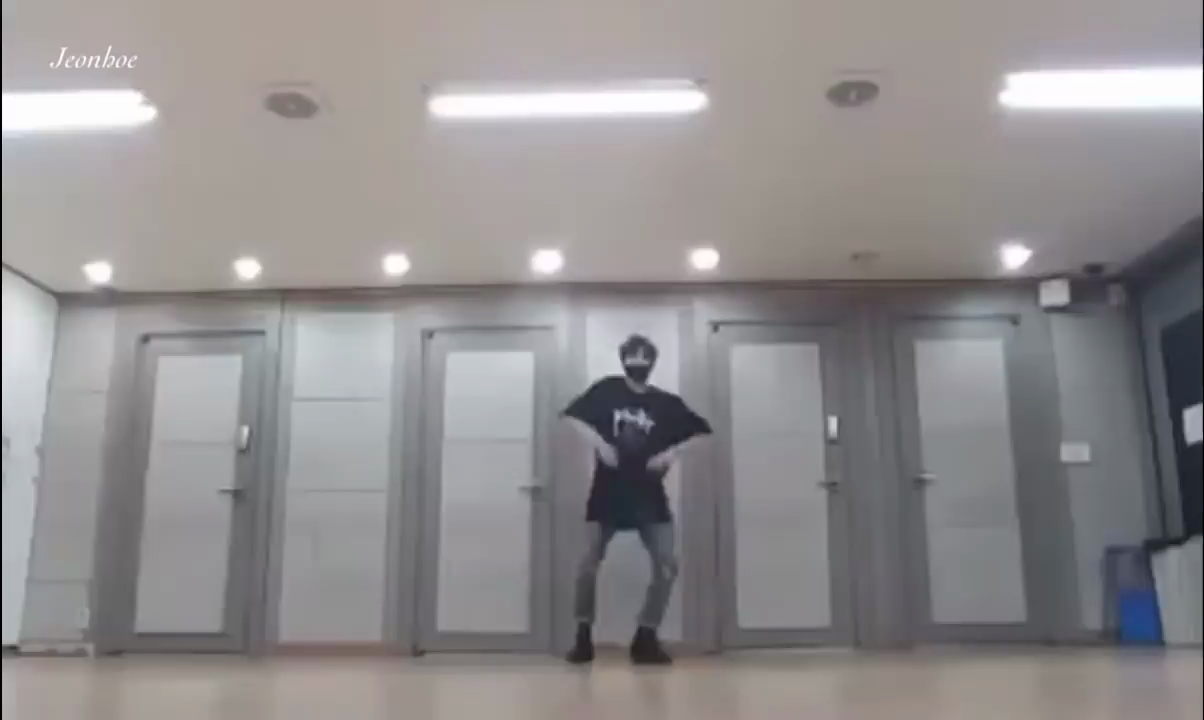
\includegraphics[width=17mm]{images/snaps/manolo_dance.png}
        & 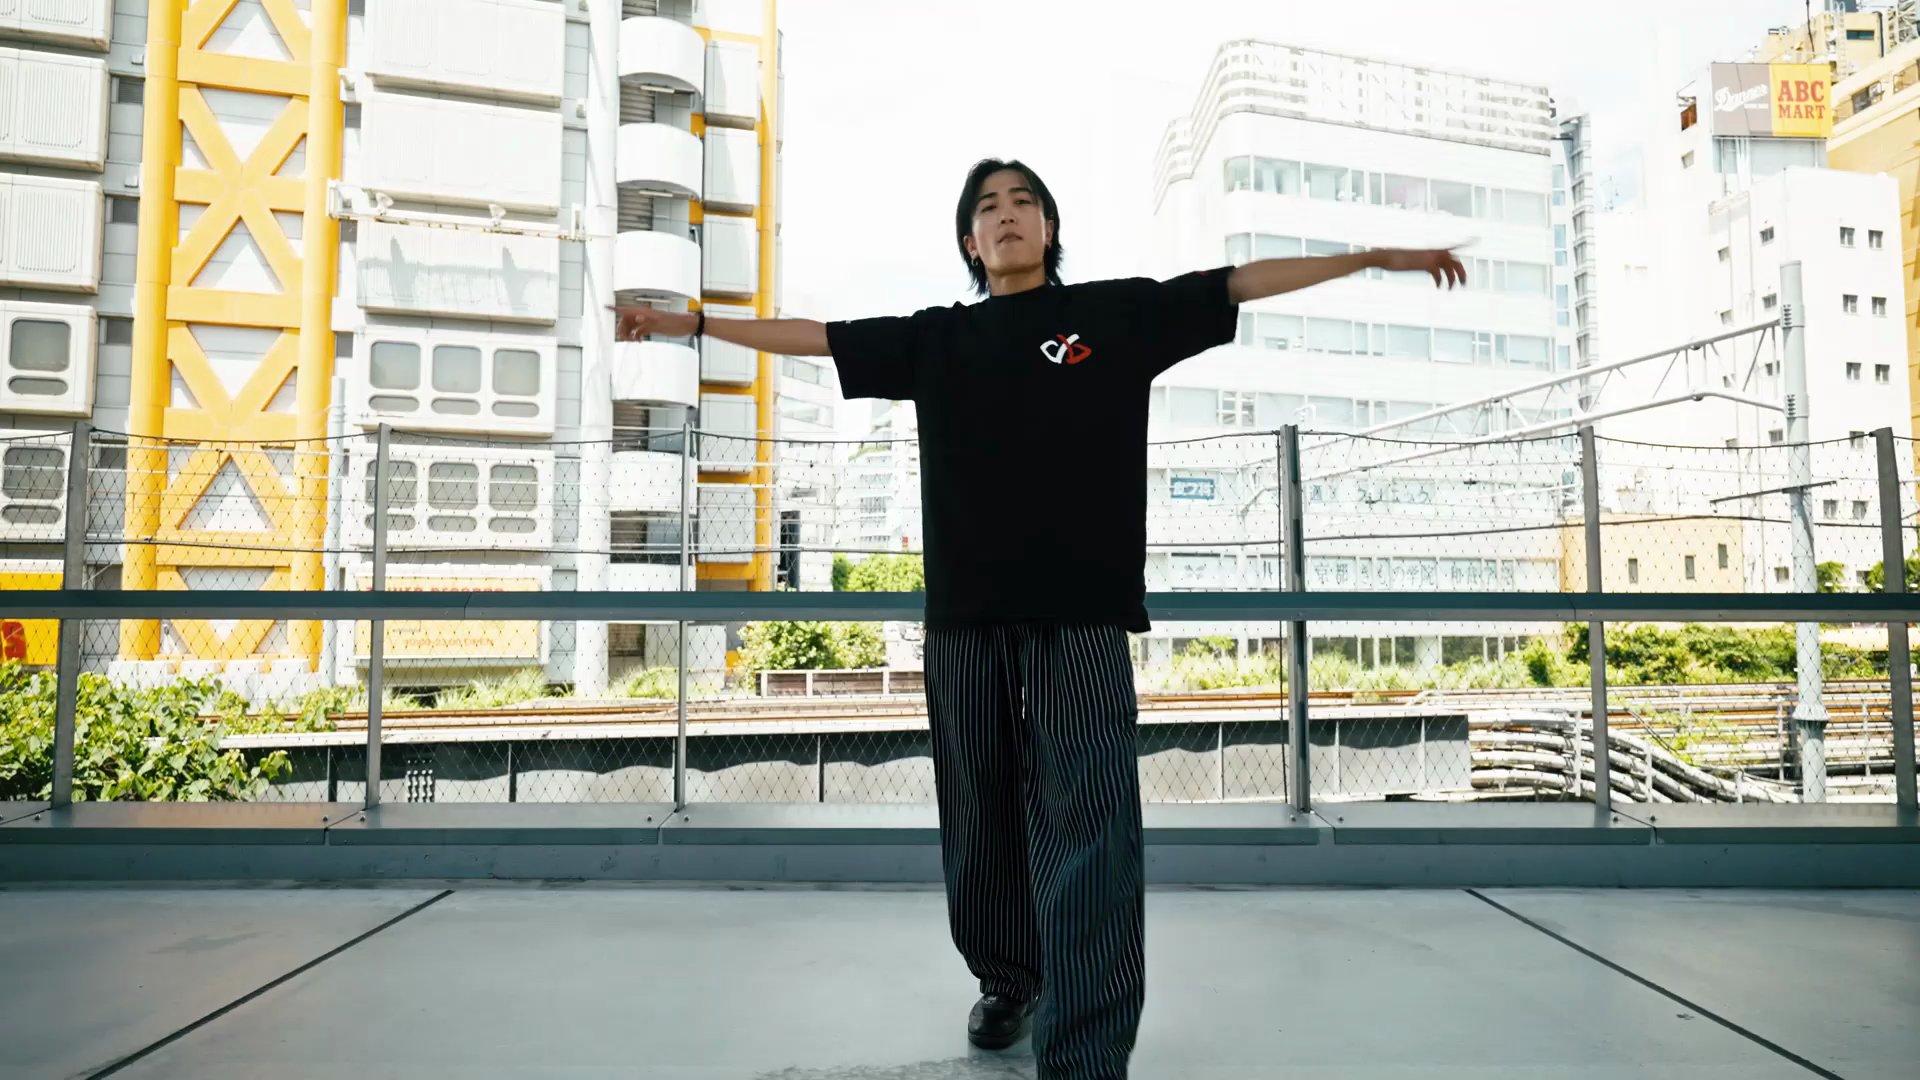
\includegraphics[width=17mm]{images/snaps/aito_dance.png}
        &
        & 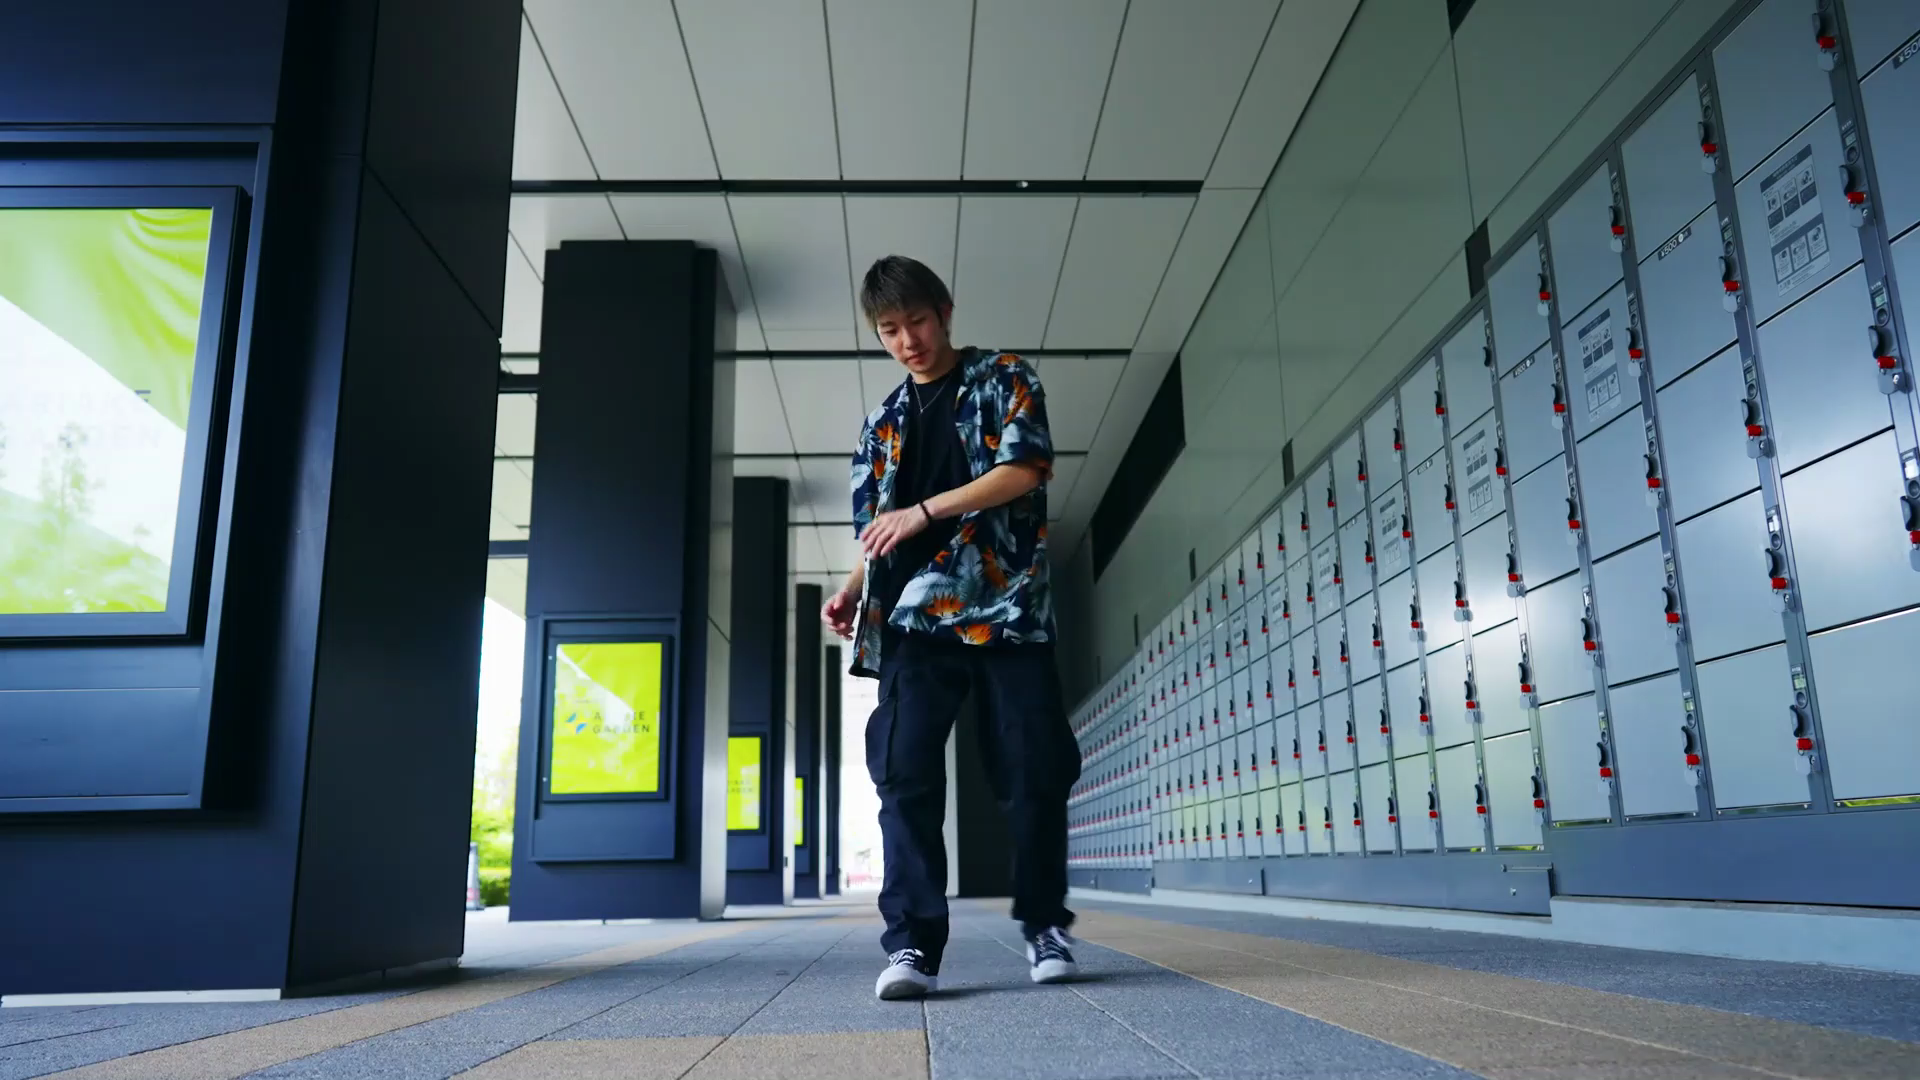
\includegraphics[width=17mm]{images/snaps/hyoga_dance.png}
        & 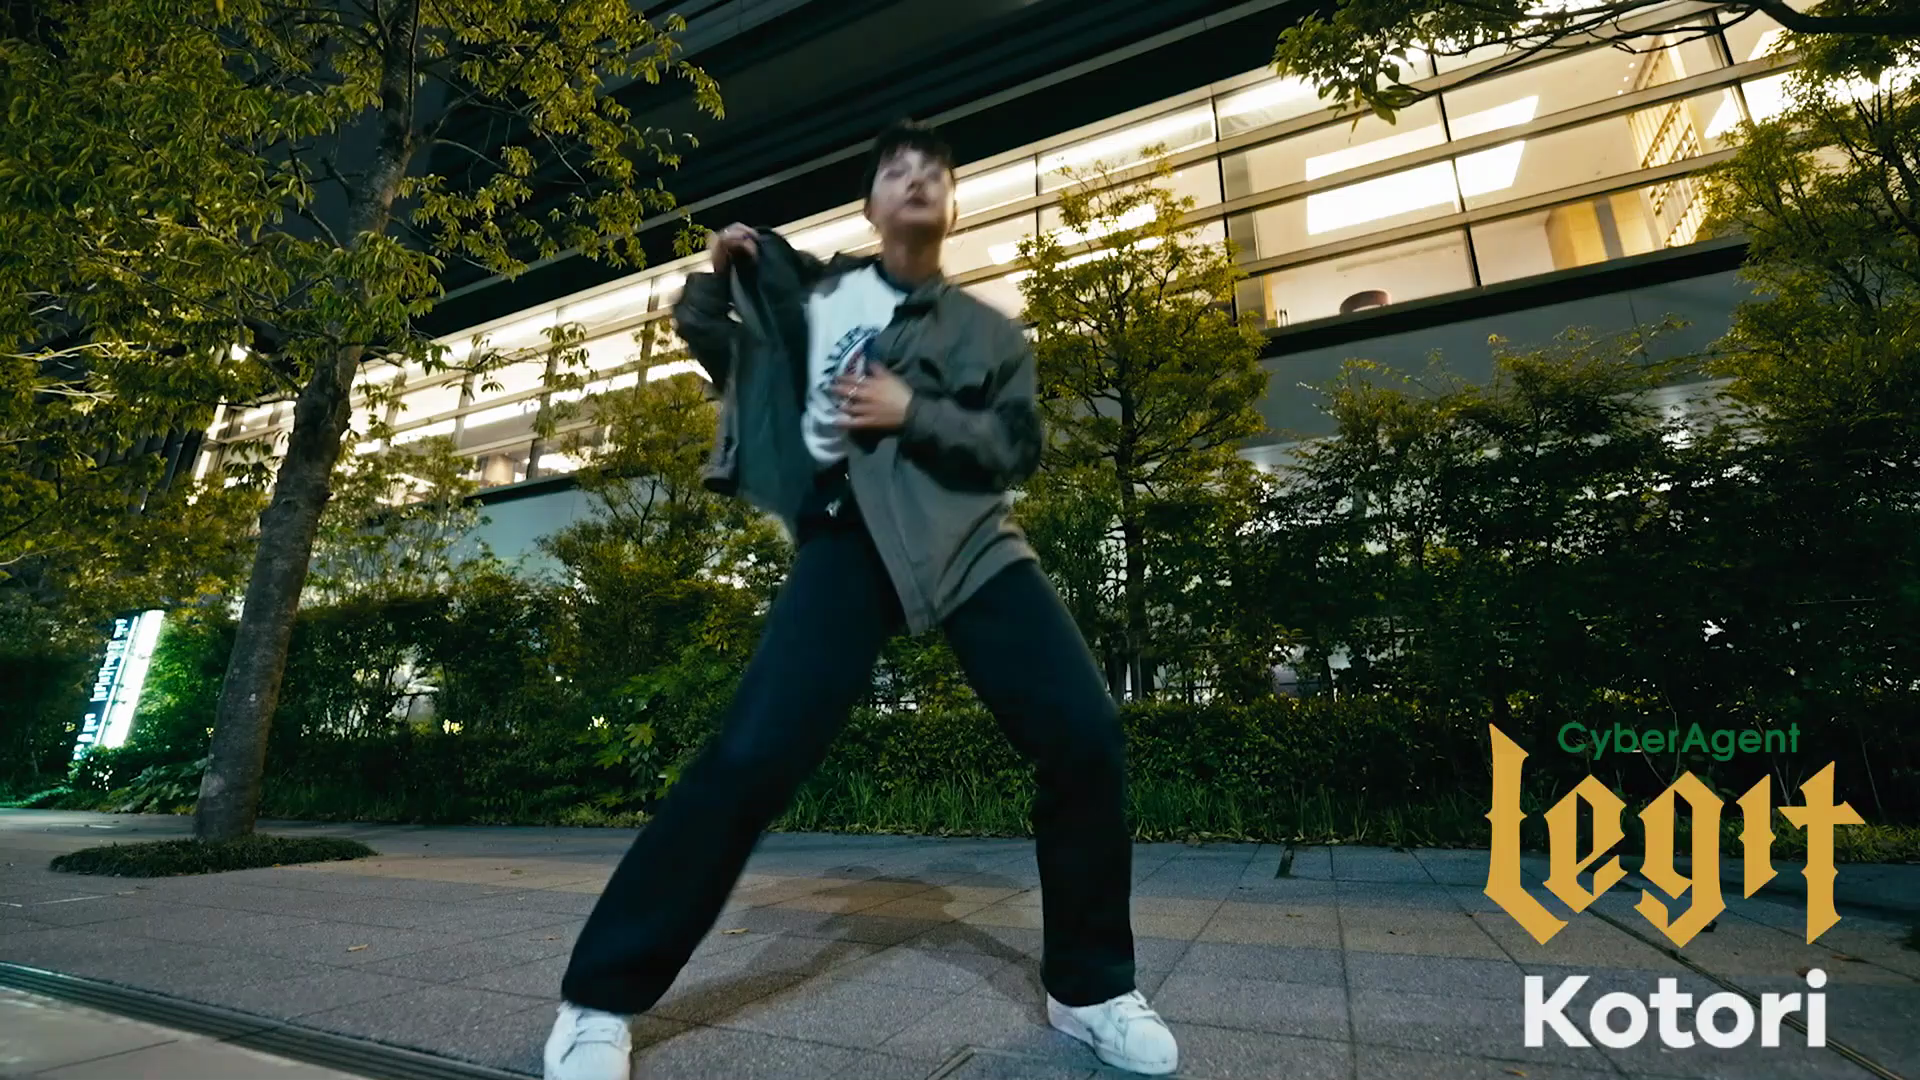
\includegraphics[width=17mm]{images/snaps/legit_dance.png}
      \\
        & \cite{manolo} & \cite{aito} & & \cite{hyoga} & \cite{legit}
      \\ \hline
        &&&&& \\
        & 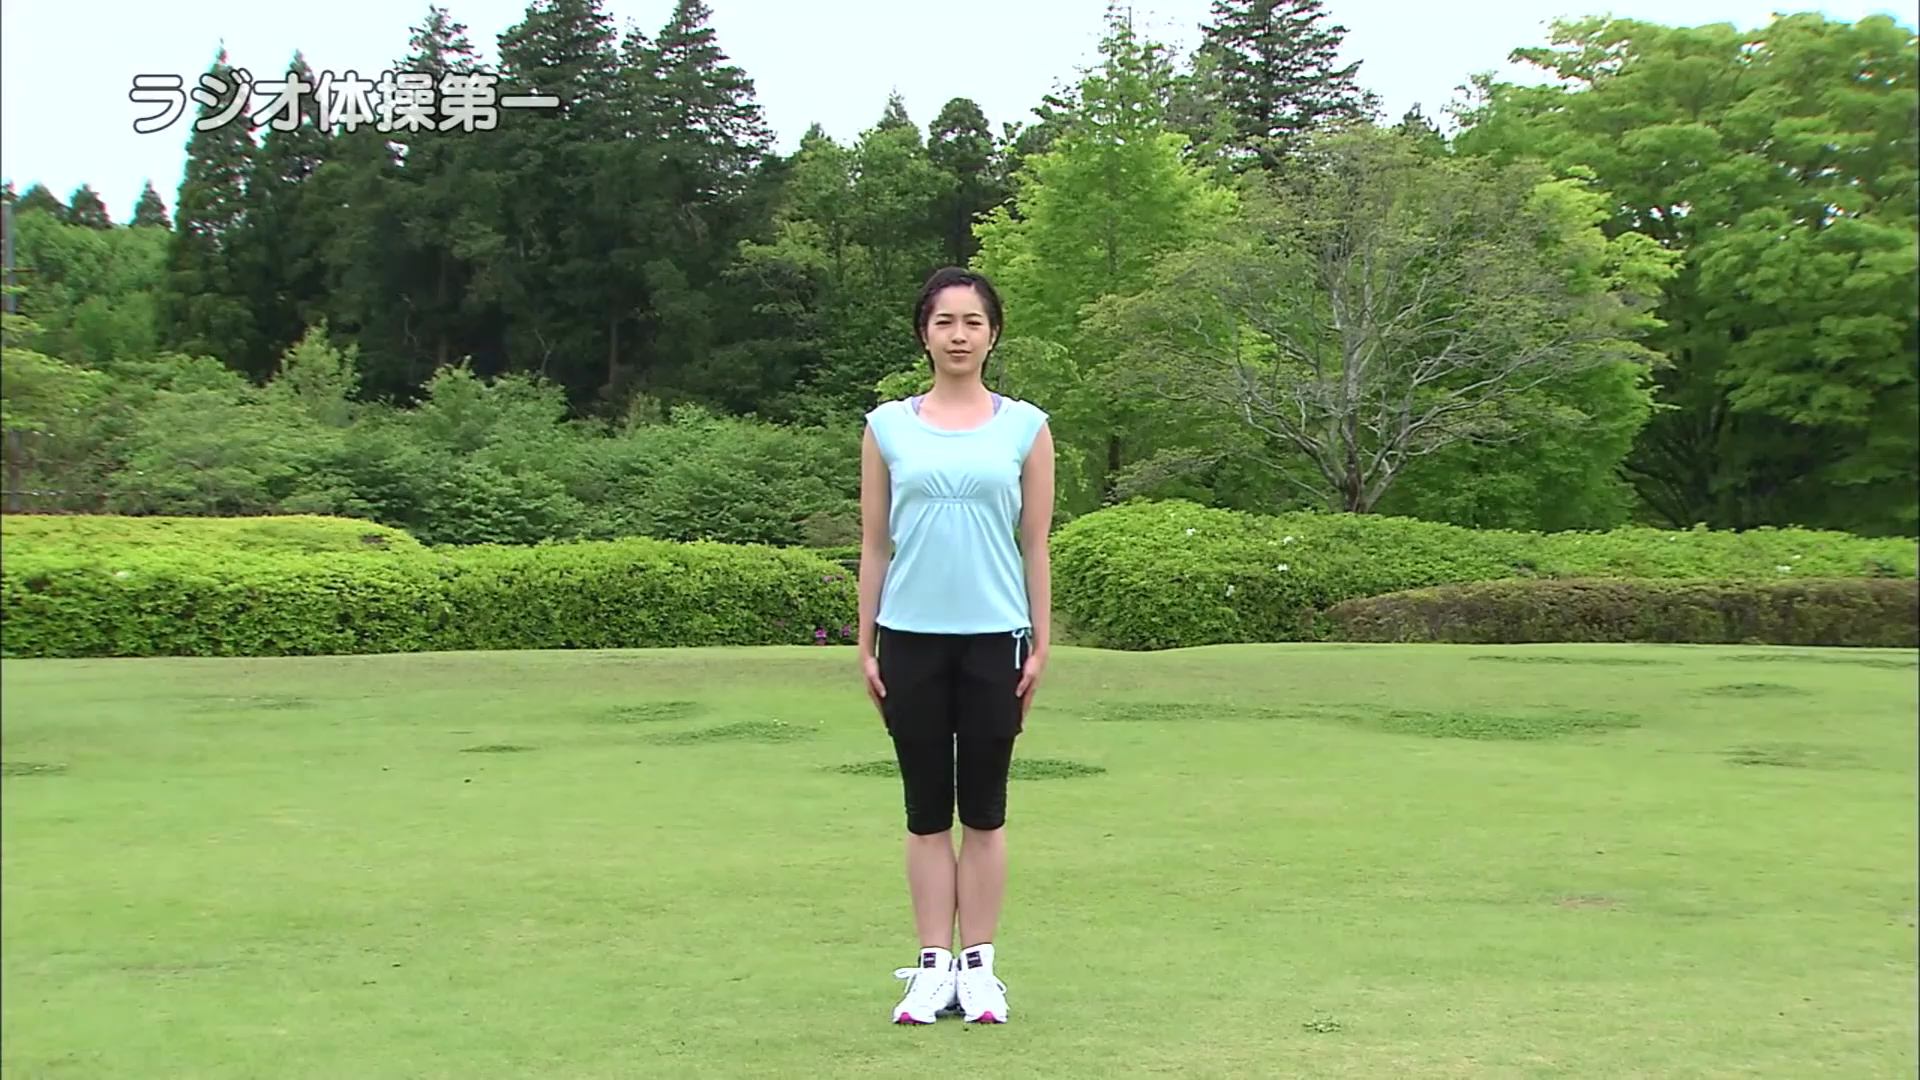
\includegraphics[width=17mm]{images/snaps/radio_exer.png}
        & 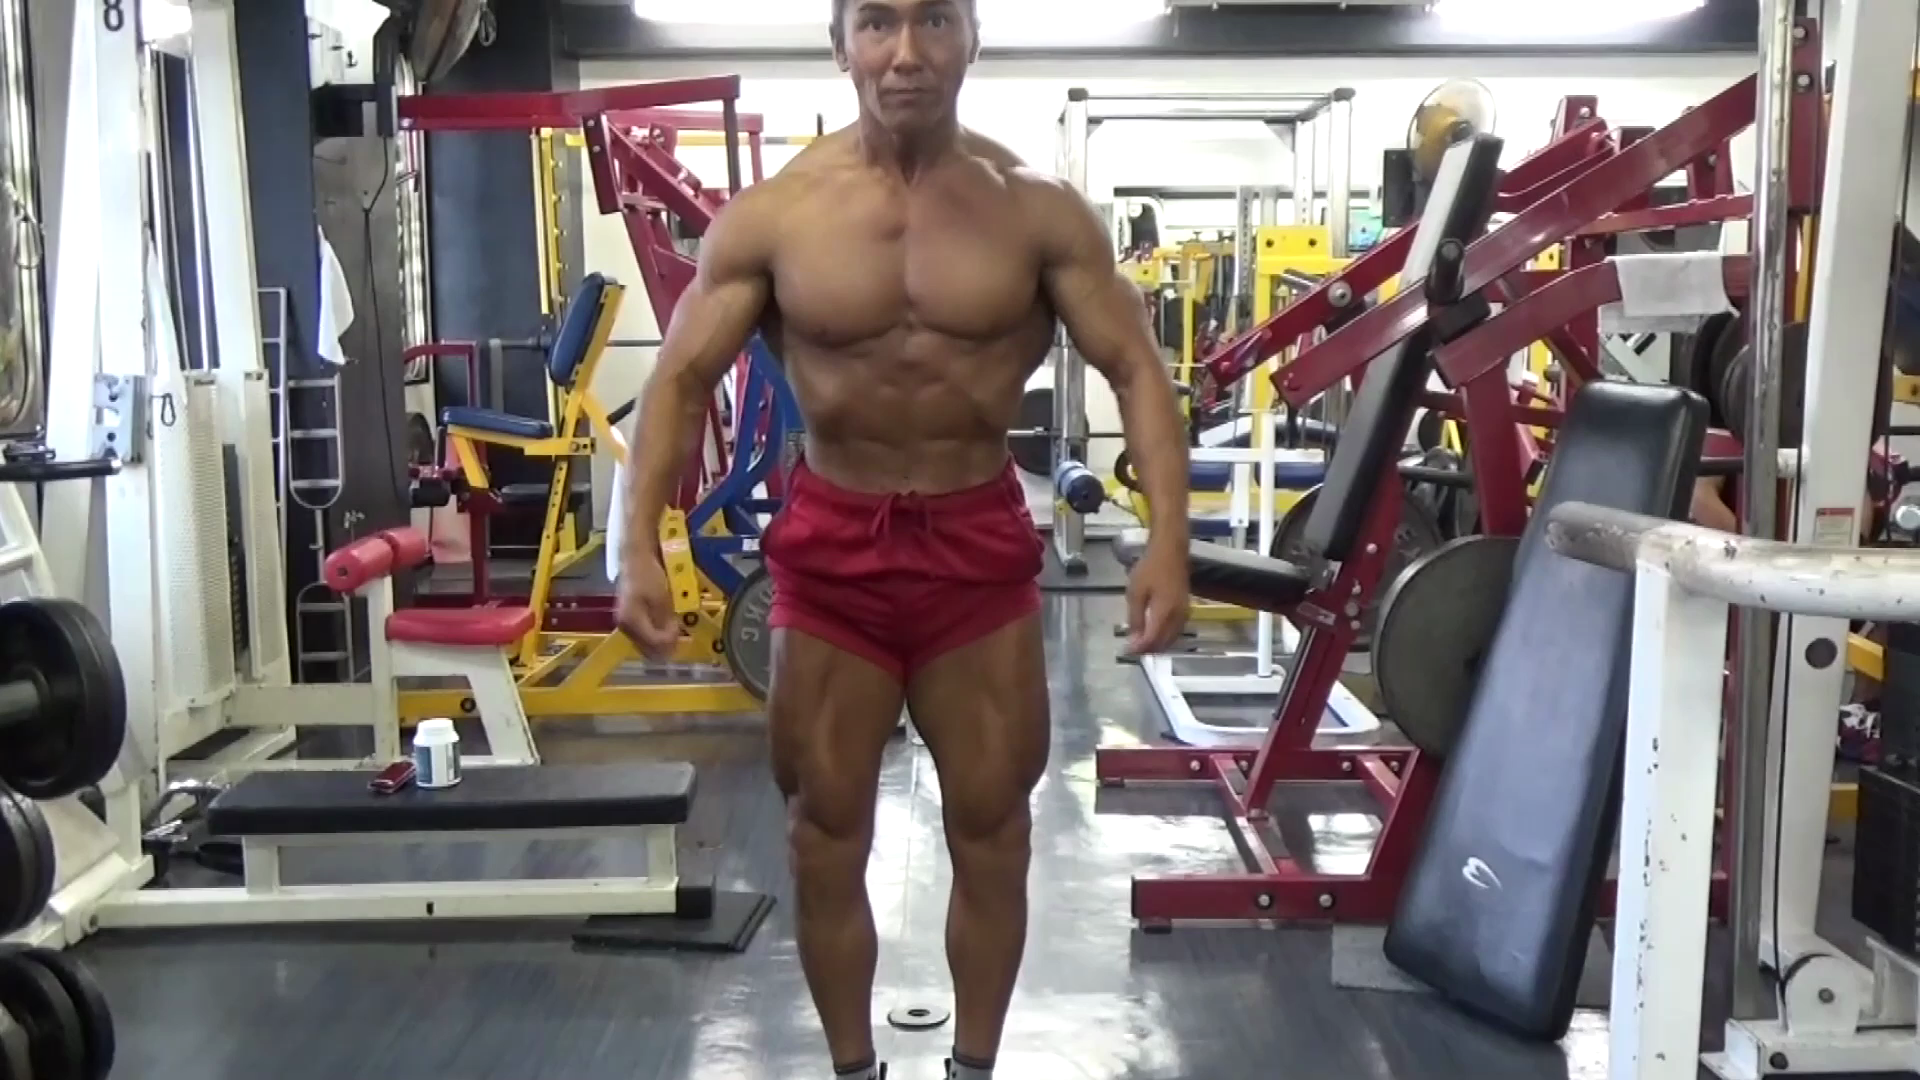
\includegraphics[width=17mm]{images/snaps/posing.png}
        & 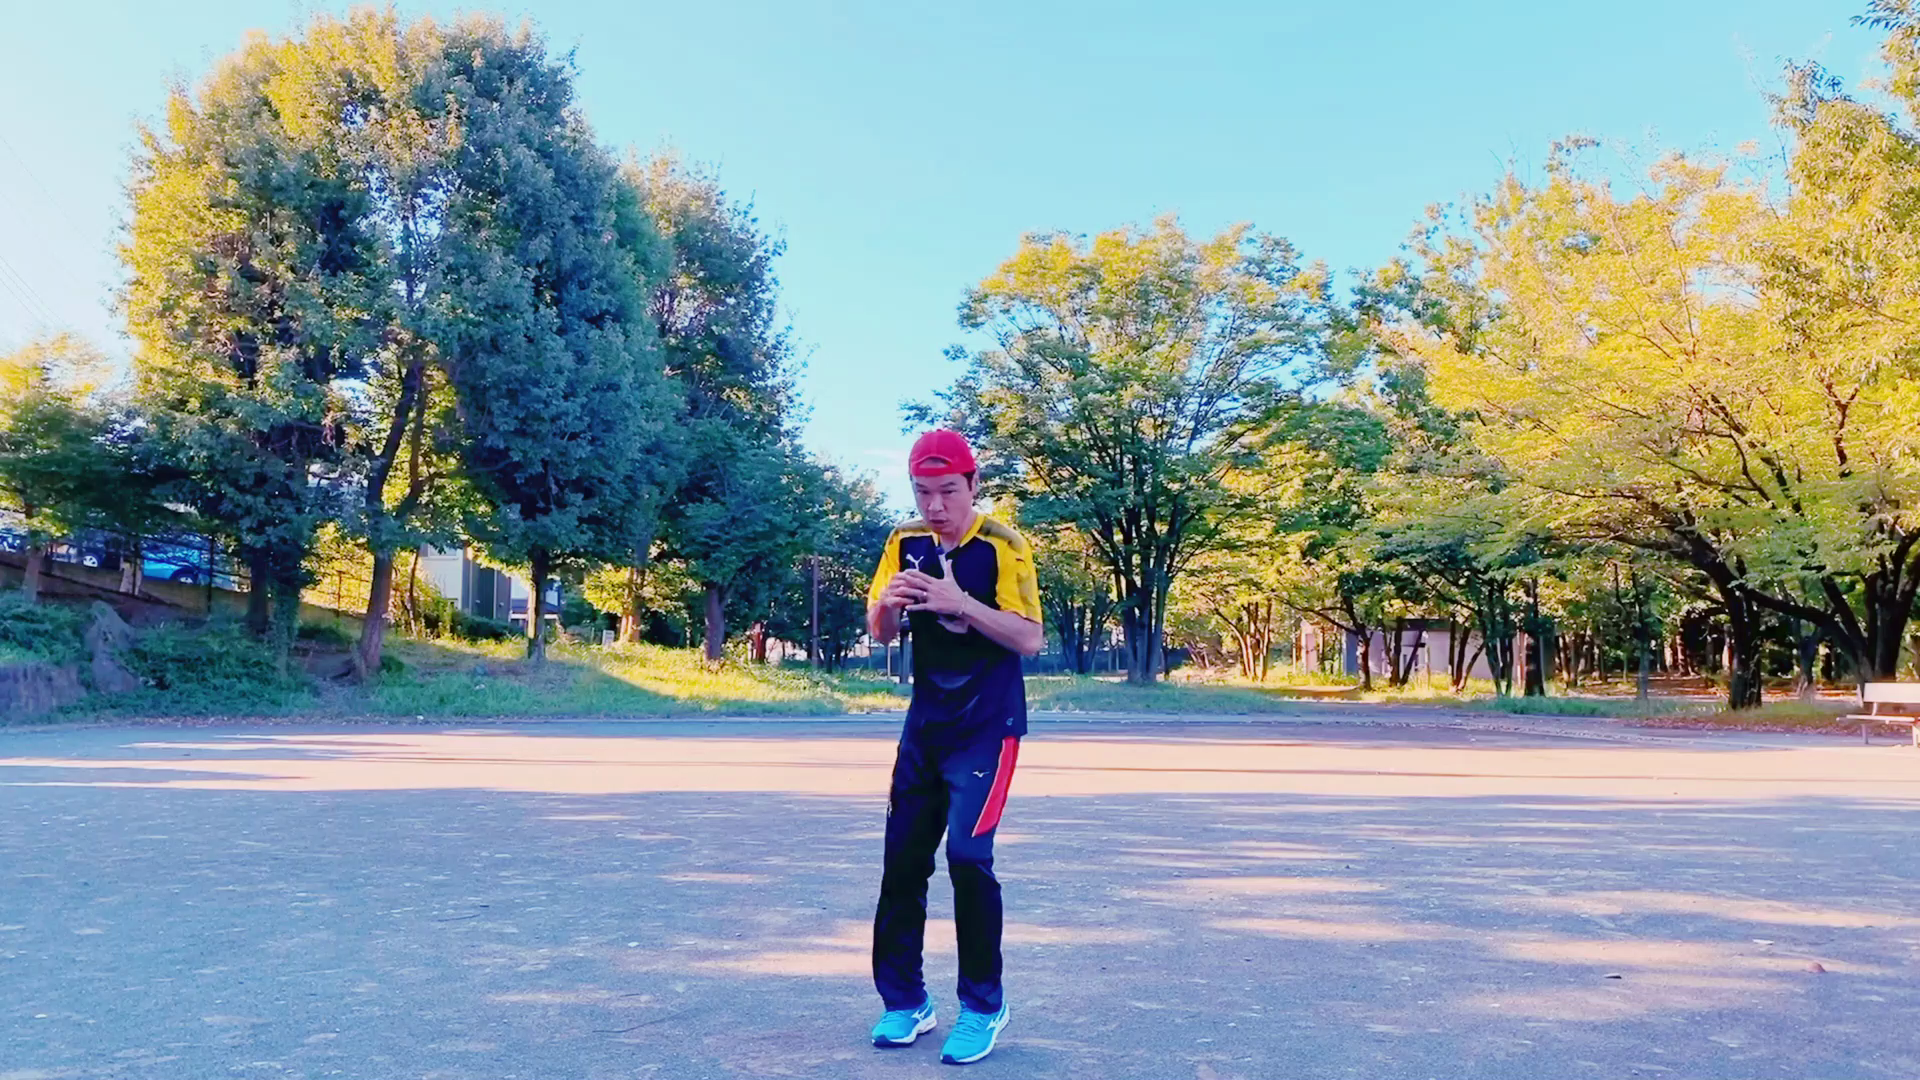
\includegraphics[width=17mm]{images/snaps/shadowboxing.png}
        & 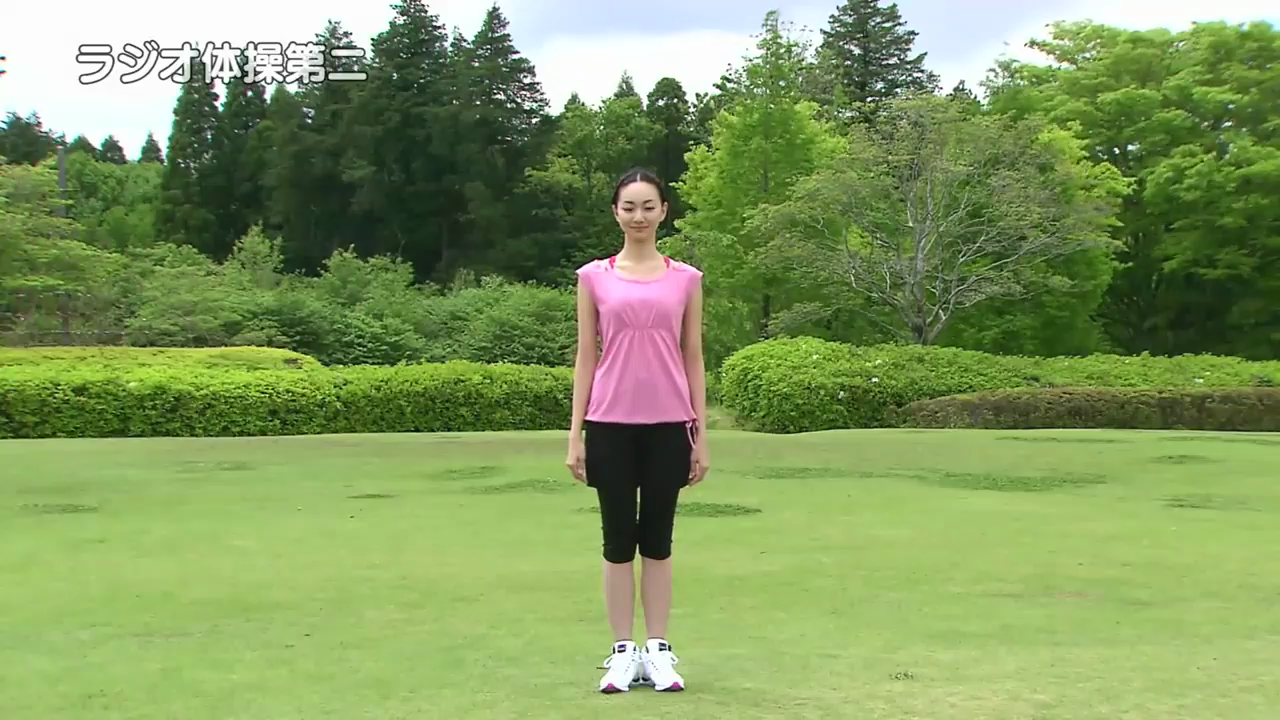
\includegraphics[width=17mm]{images/snaps/radio_exer_2.png}
        &
      \\
      その他の動作 & \cite{radio} & \cite{posing} & \cite{boxing} & \cite{radio2} &
      \\
        & 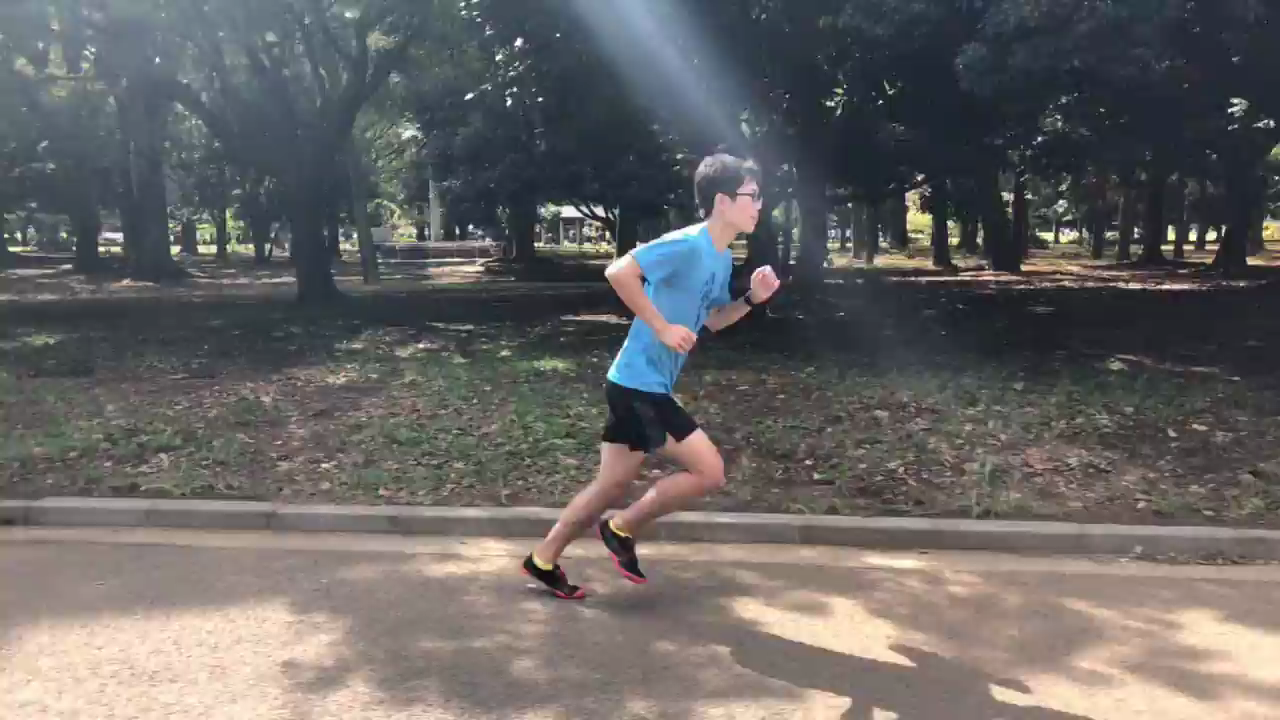
\includegraphics[width=17mm]{images/snaps/running.png}
        & 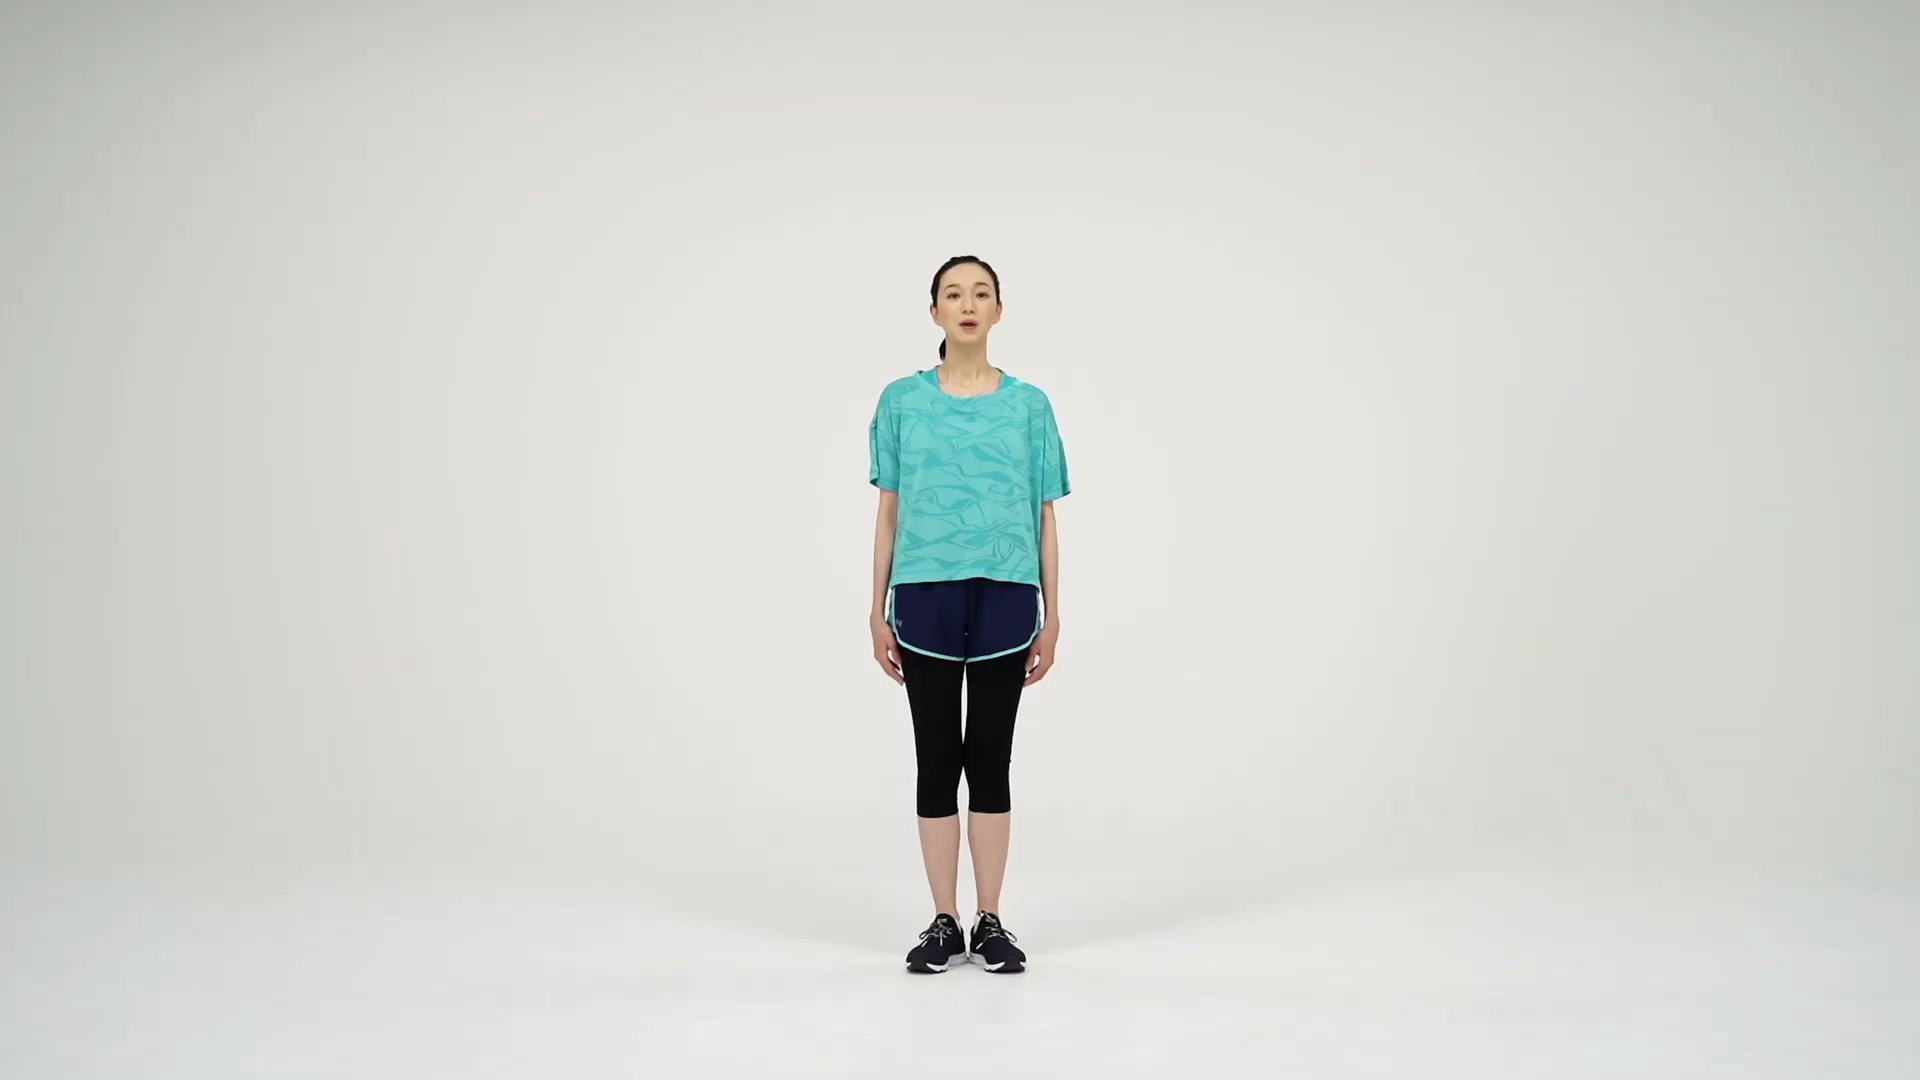
\includegraphics[width=17mm]{images/snaps/shinkokyu.png}
        & 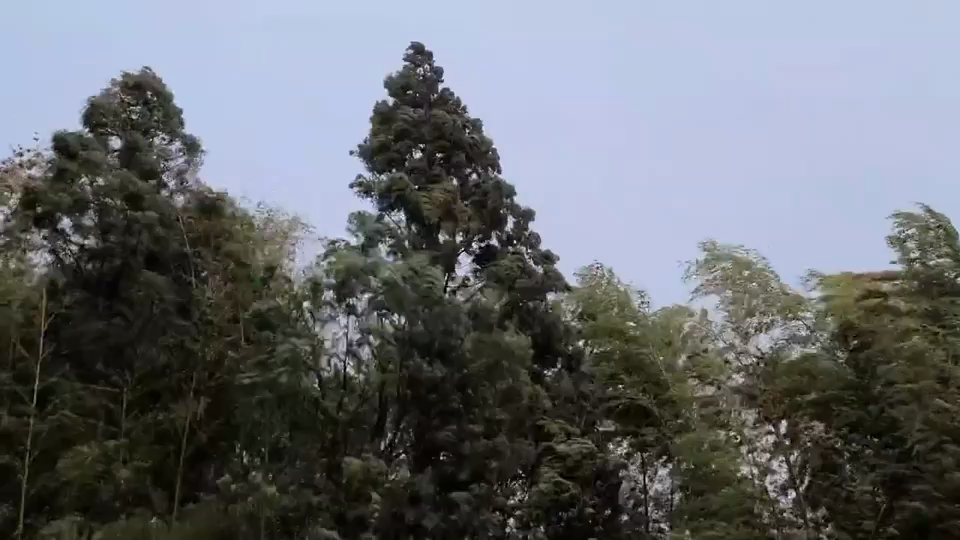
\includegraphics[width=17mm]{images/snaps/leaves.png}
        &
        &
      \\
        & \cite{running} & \cite{shinkokyu} & \cite{leaves} & &
      \\ \hline
    \end{tabular}
  \end{center}
  \caption{使用した動画データ}
  \label{video_data}
\end{table}
\clearpage

\begin{figure}[t]
  \begin{center}
    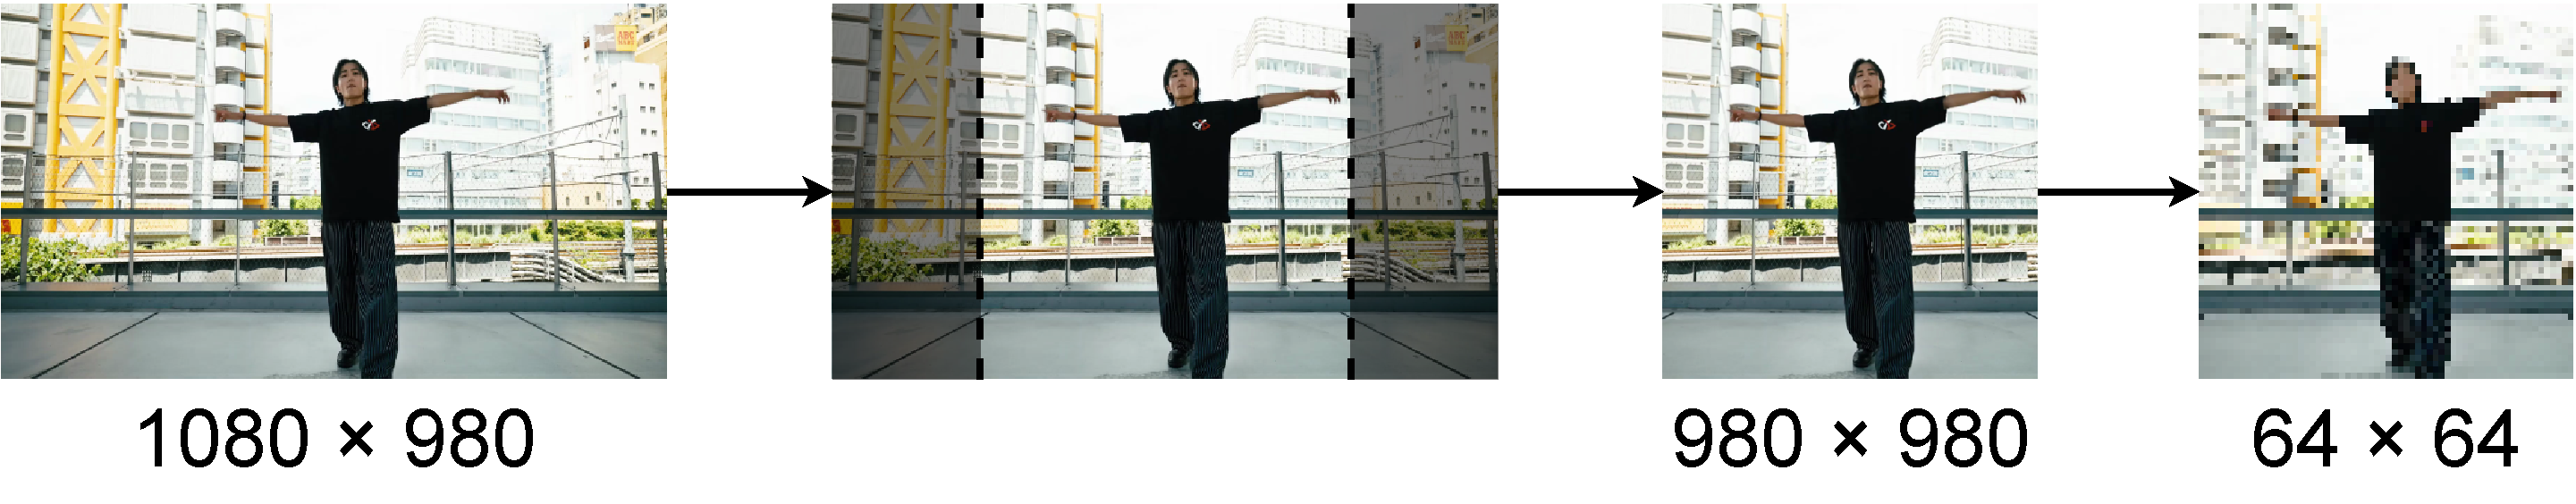
\includegraphics[width=120mm]{images/chart/resize.pdf}
  \end{center}
  \caption{動画の縮小例}
  \label{resize}
\end{figure}

動画の編集方法は,まず,動画サイズを均一にするために
図\ref{resize}のように縦横64ピクセルに縮小する.
縦横短い方を基準に長い方の両端を切り出し,OpenCVのresize関数\cite{resize}を使用した.
畳み込みでは正方形のフィルタを用いるため,動画サイズを正方形にする必要があった.
動画を確認した結果,64ピクセルが動作が確認できる最も小さなサイズであった.

次に,図\ref{binary}のように動画を二値化する.
グレースケール化した動画の1フレームごとの画像全体の平均を計算し,
その平均より輝度の低いピクセルを255,高いピクセルを0にする.

最後に図\ref{choice}のように白画素の制限を行う.
二値化した動画の1ピクセルのフレーム長方向の配列を取り出した.
その配列の平均を取り,255/4に近い順で500画素まで白画素を採用した.
対象が黒画素であった場合はカウントしない.
閾値255/4は複数の動画に対し閾値を変えながら制限処理を行なった中で,
多くの動画で最も効果的に人体の輪郭を得ることができたため,このような値を用いた.

検証段階として,動画データをそのままネットワークにかけて学習した結果,精度が
ほとんど取れなかった原因として動画データの不統一にあると考え,
二値に限定し,各ピクセル,動画全体のデータを均一にすることで学習の効率を高めることを試みた.

\begin{figure}[b]
  \begin{center}
    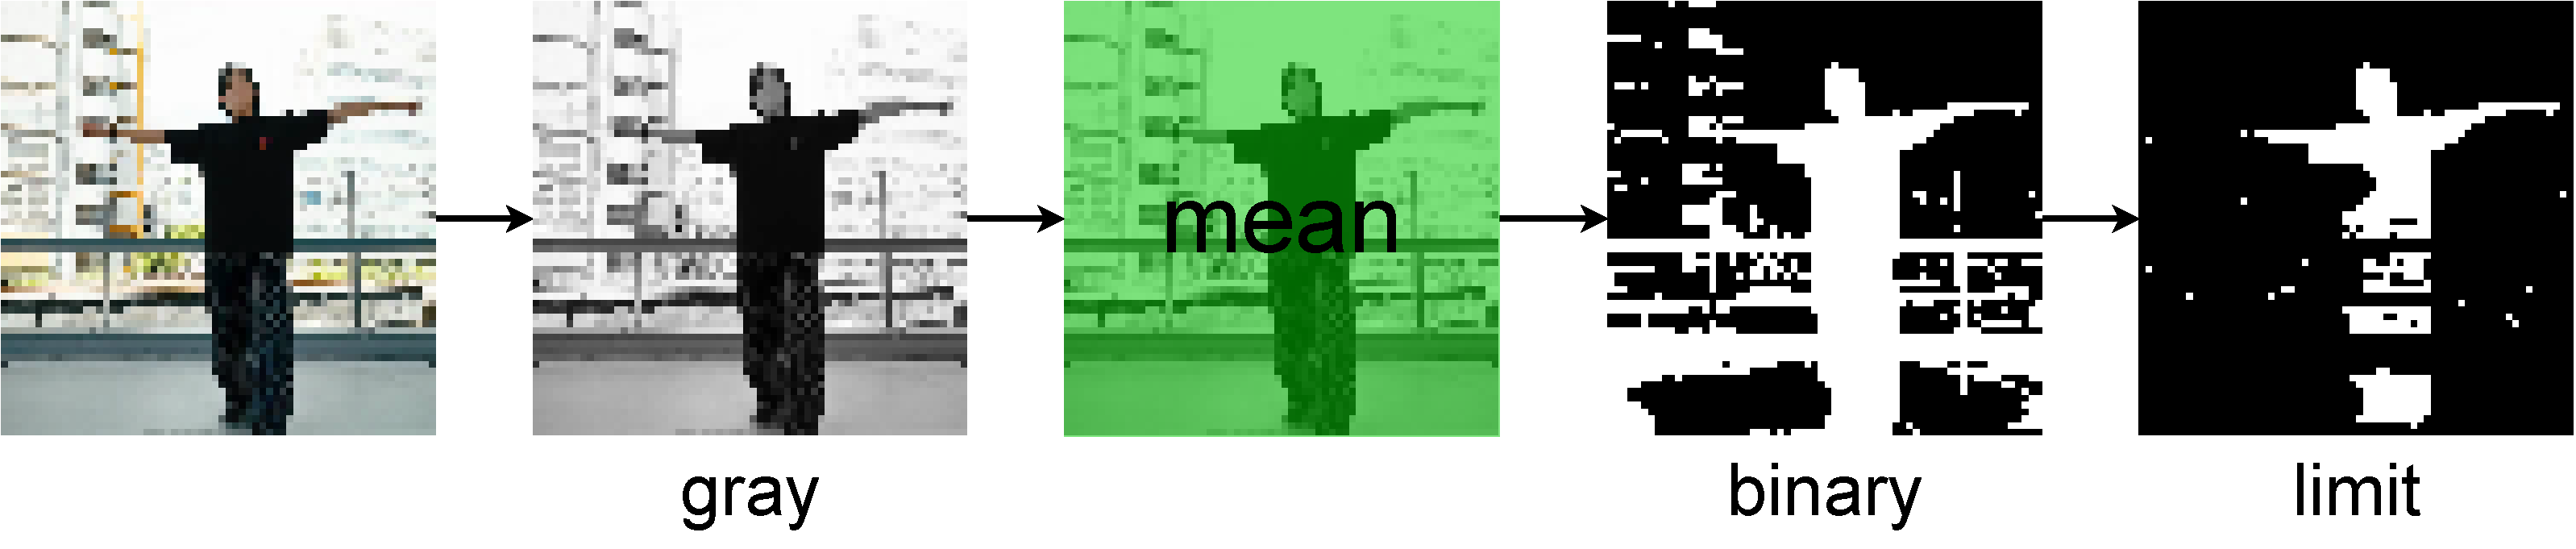
\includegraphics[width=120mm]{images/chart/binary.pdf}
  \end{center}
  \caption{動画の二値化例}
  \label{binary}
\end{figure}
\clearpage

\begin{figure}[t]
  \begin{center}
    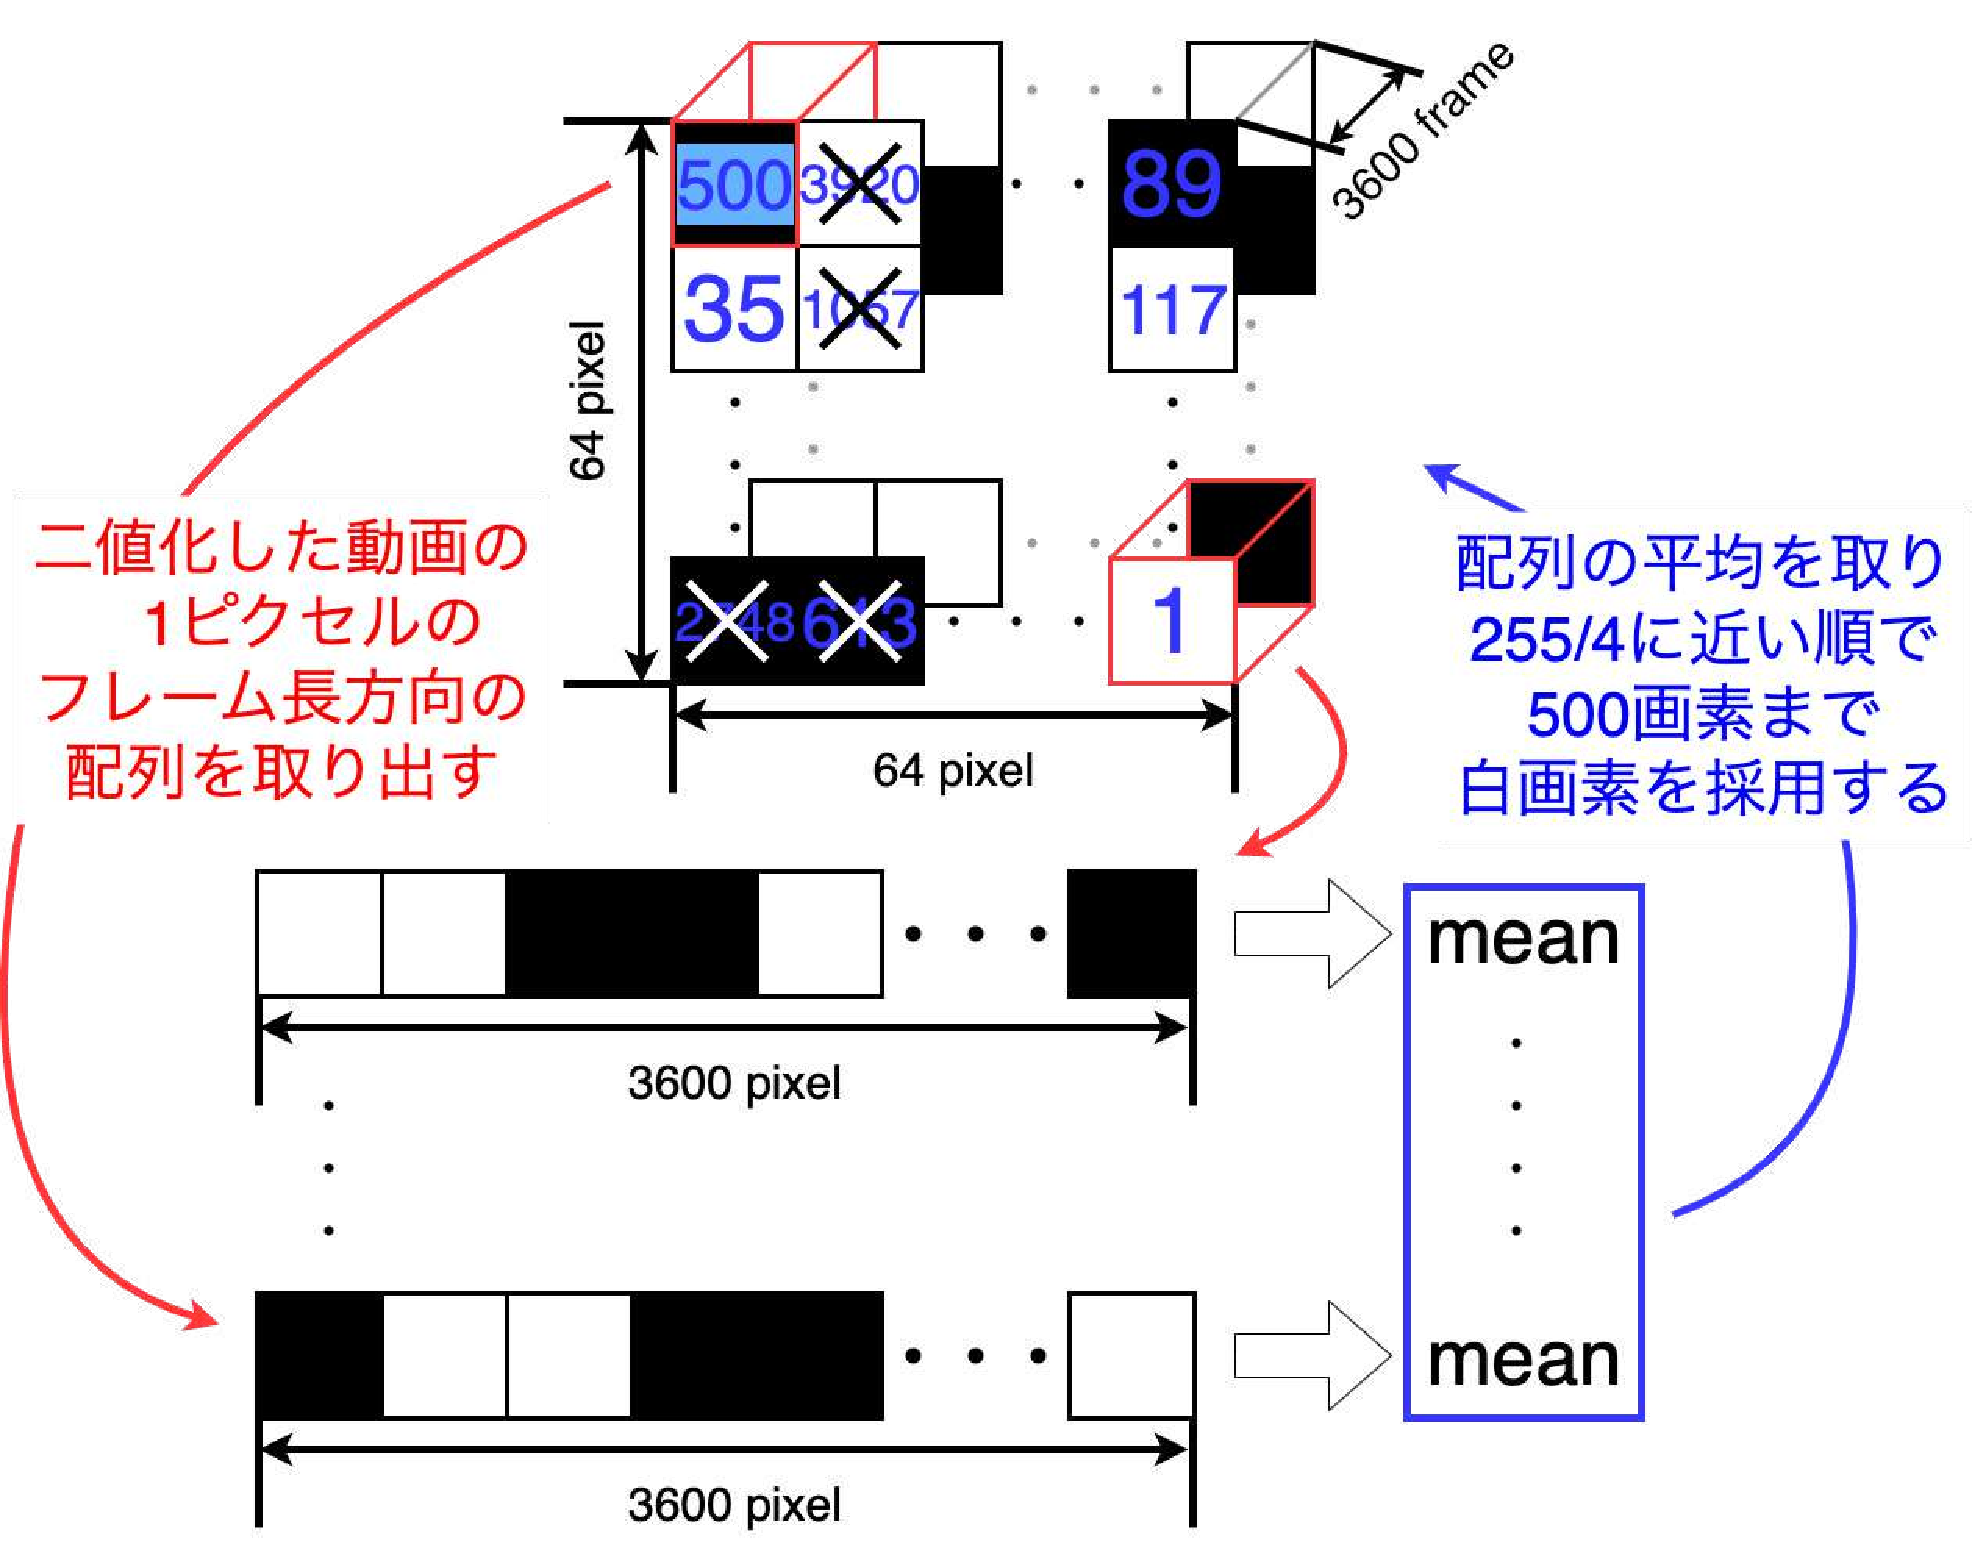
\includegraphics[width=120mm]{images/chart/choice.pdf}
  \end{center}
  \caption{白画素の制限方法}
  \label{choice}
\end{figure}

図\ref{choice}のように動画長方向の各ピクセルに注目する理由は,
対象の画素の変化量を知りたかったからである.
例えば手先が移動している場合,手先が元あった場所は背景色に変化するはずである.
逆に移動先では背景色が手先の色に変化する.
第1章,論文構成でも述べた通り,今回の研究では動作から優美さを抽出したいので,
動作の変化,動画データでは画素の変化を取り出したいと言い換えることができる.
そのために,1フレームごとの静止した画像ではなく,各ピクセルの動画長方向のデータを
用いることでデータを動作として扱うことができ,その平均を閾値で順序付けることで
目標とするに最も近い動作のみを抽出することができると考えた.
\clearpage

\subsection{ネットワーク構造}
編集した動画をそのまま使用するとフレーム数が多いので動画を複数に分割することを考えた.
図\ref{range}のように乱数を得た.乱数を視点として指定のフレーム長を切り取った.
それらをバッチ数まで集めた.バッチとは,データをひとまとめにして同時に学習させることである.
乱数は各データ毎に個別に作成している.

動画群は結合して一つのデータとして扱うため,切り取る範囲が動画の繋ぎ目と被る可能性がある.
それを防ぐため,図\ref{decide_rand}のように予めそれぞれの動画長方向のフレームを
動画群から見た絶対数で保存しておく.指定した乱数がそれらの数値-指定フレームであった場合,
乱数を指定フレーム分追加することで再計算することなく固有の動画から指定範囲切り抜くことができる.

この手法はViViTから着想を得た.ViViTでは動画を指定フレーム,指定ピクセルの
立方体で切り出し,Transformer Encoderにかけるという手法を取っている.
切り取った動画を検証するので動画全体を検証することはできないが,フレームを細かく分割することで
優美さ特定がより円滑に進むと考えた.

\begin{figure}[b]
  \begin{center}
    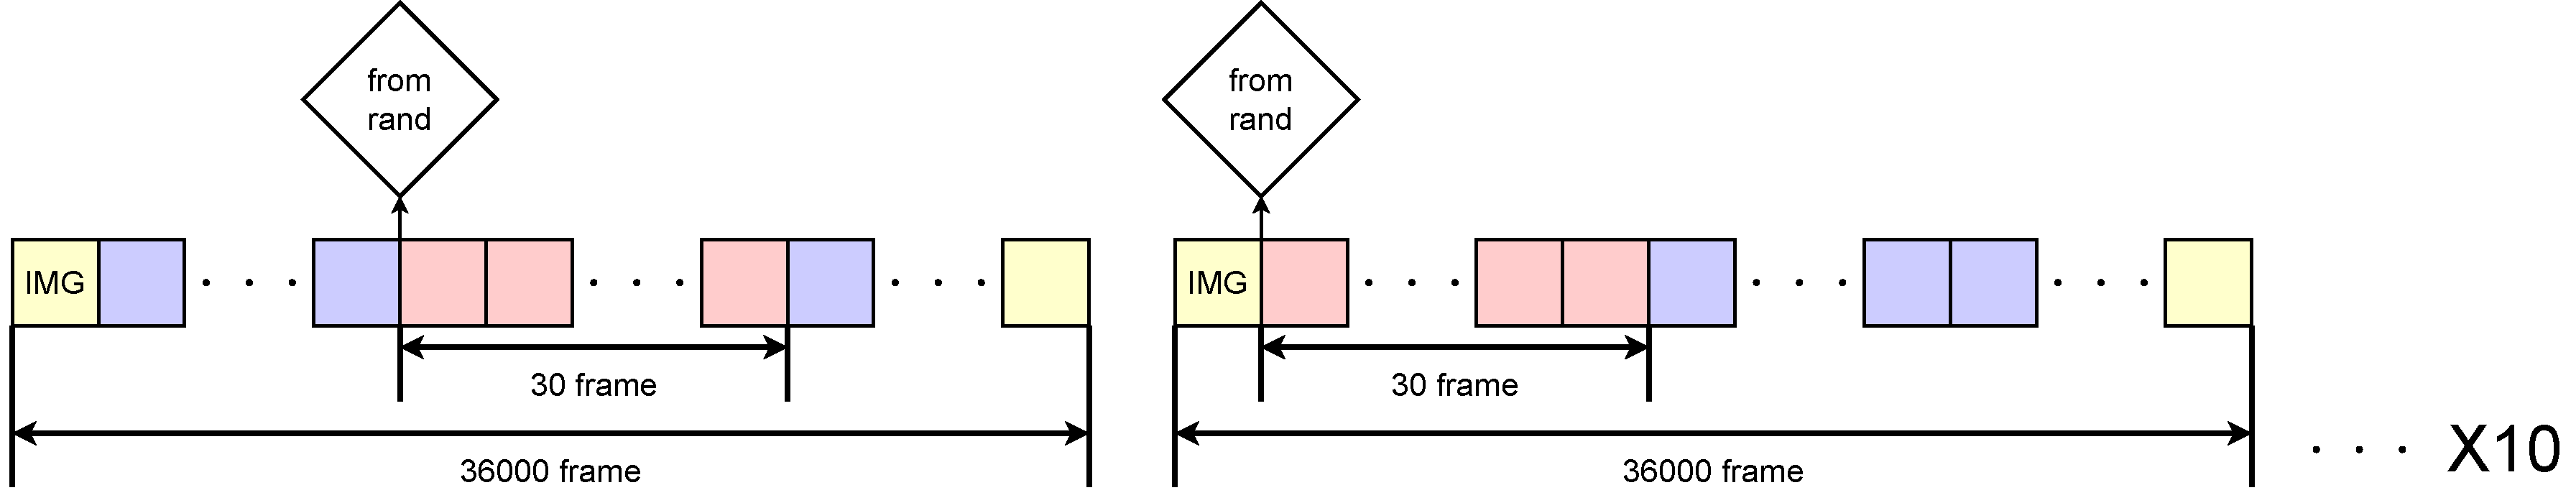
\includegraphics[width=120mm]{images/chart/range.pdf}
  \end{center}
  \caption{入力動画の分割方法}
  \label{range}
\end{figure}

\begin{figure}[b]
  \begin{center}
    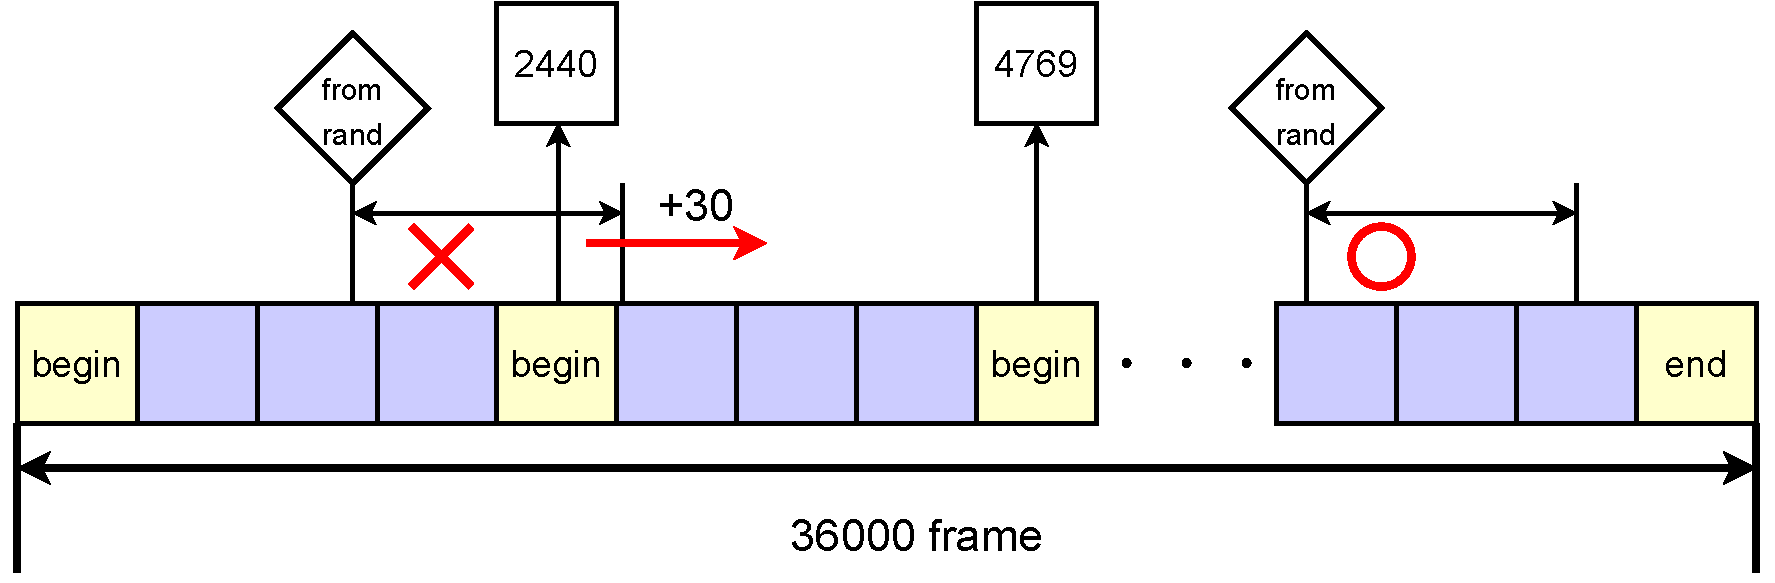
\includegraphics[width=120mm]{images/chart/decide_rand.pdf}
  \end{center}
  \caption{乱数の決定方法}
  \label{decide_rand}
\end{figure}
\clearpage

\begin{figure}[t]
  \begin{center}
    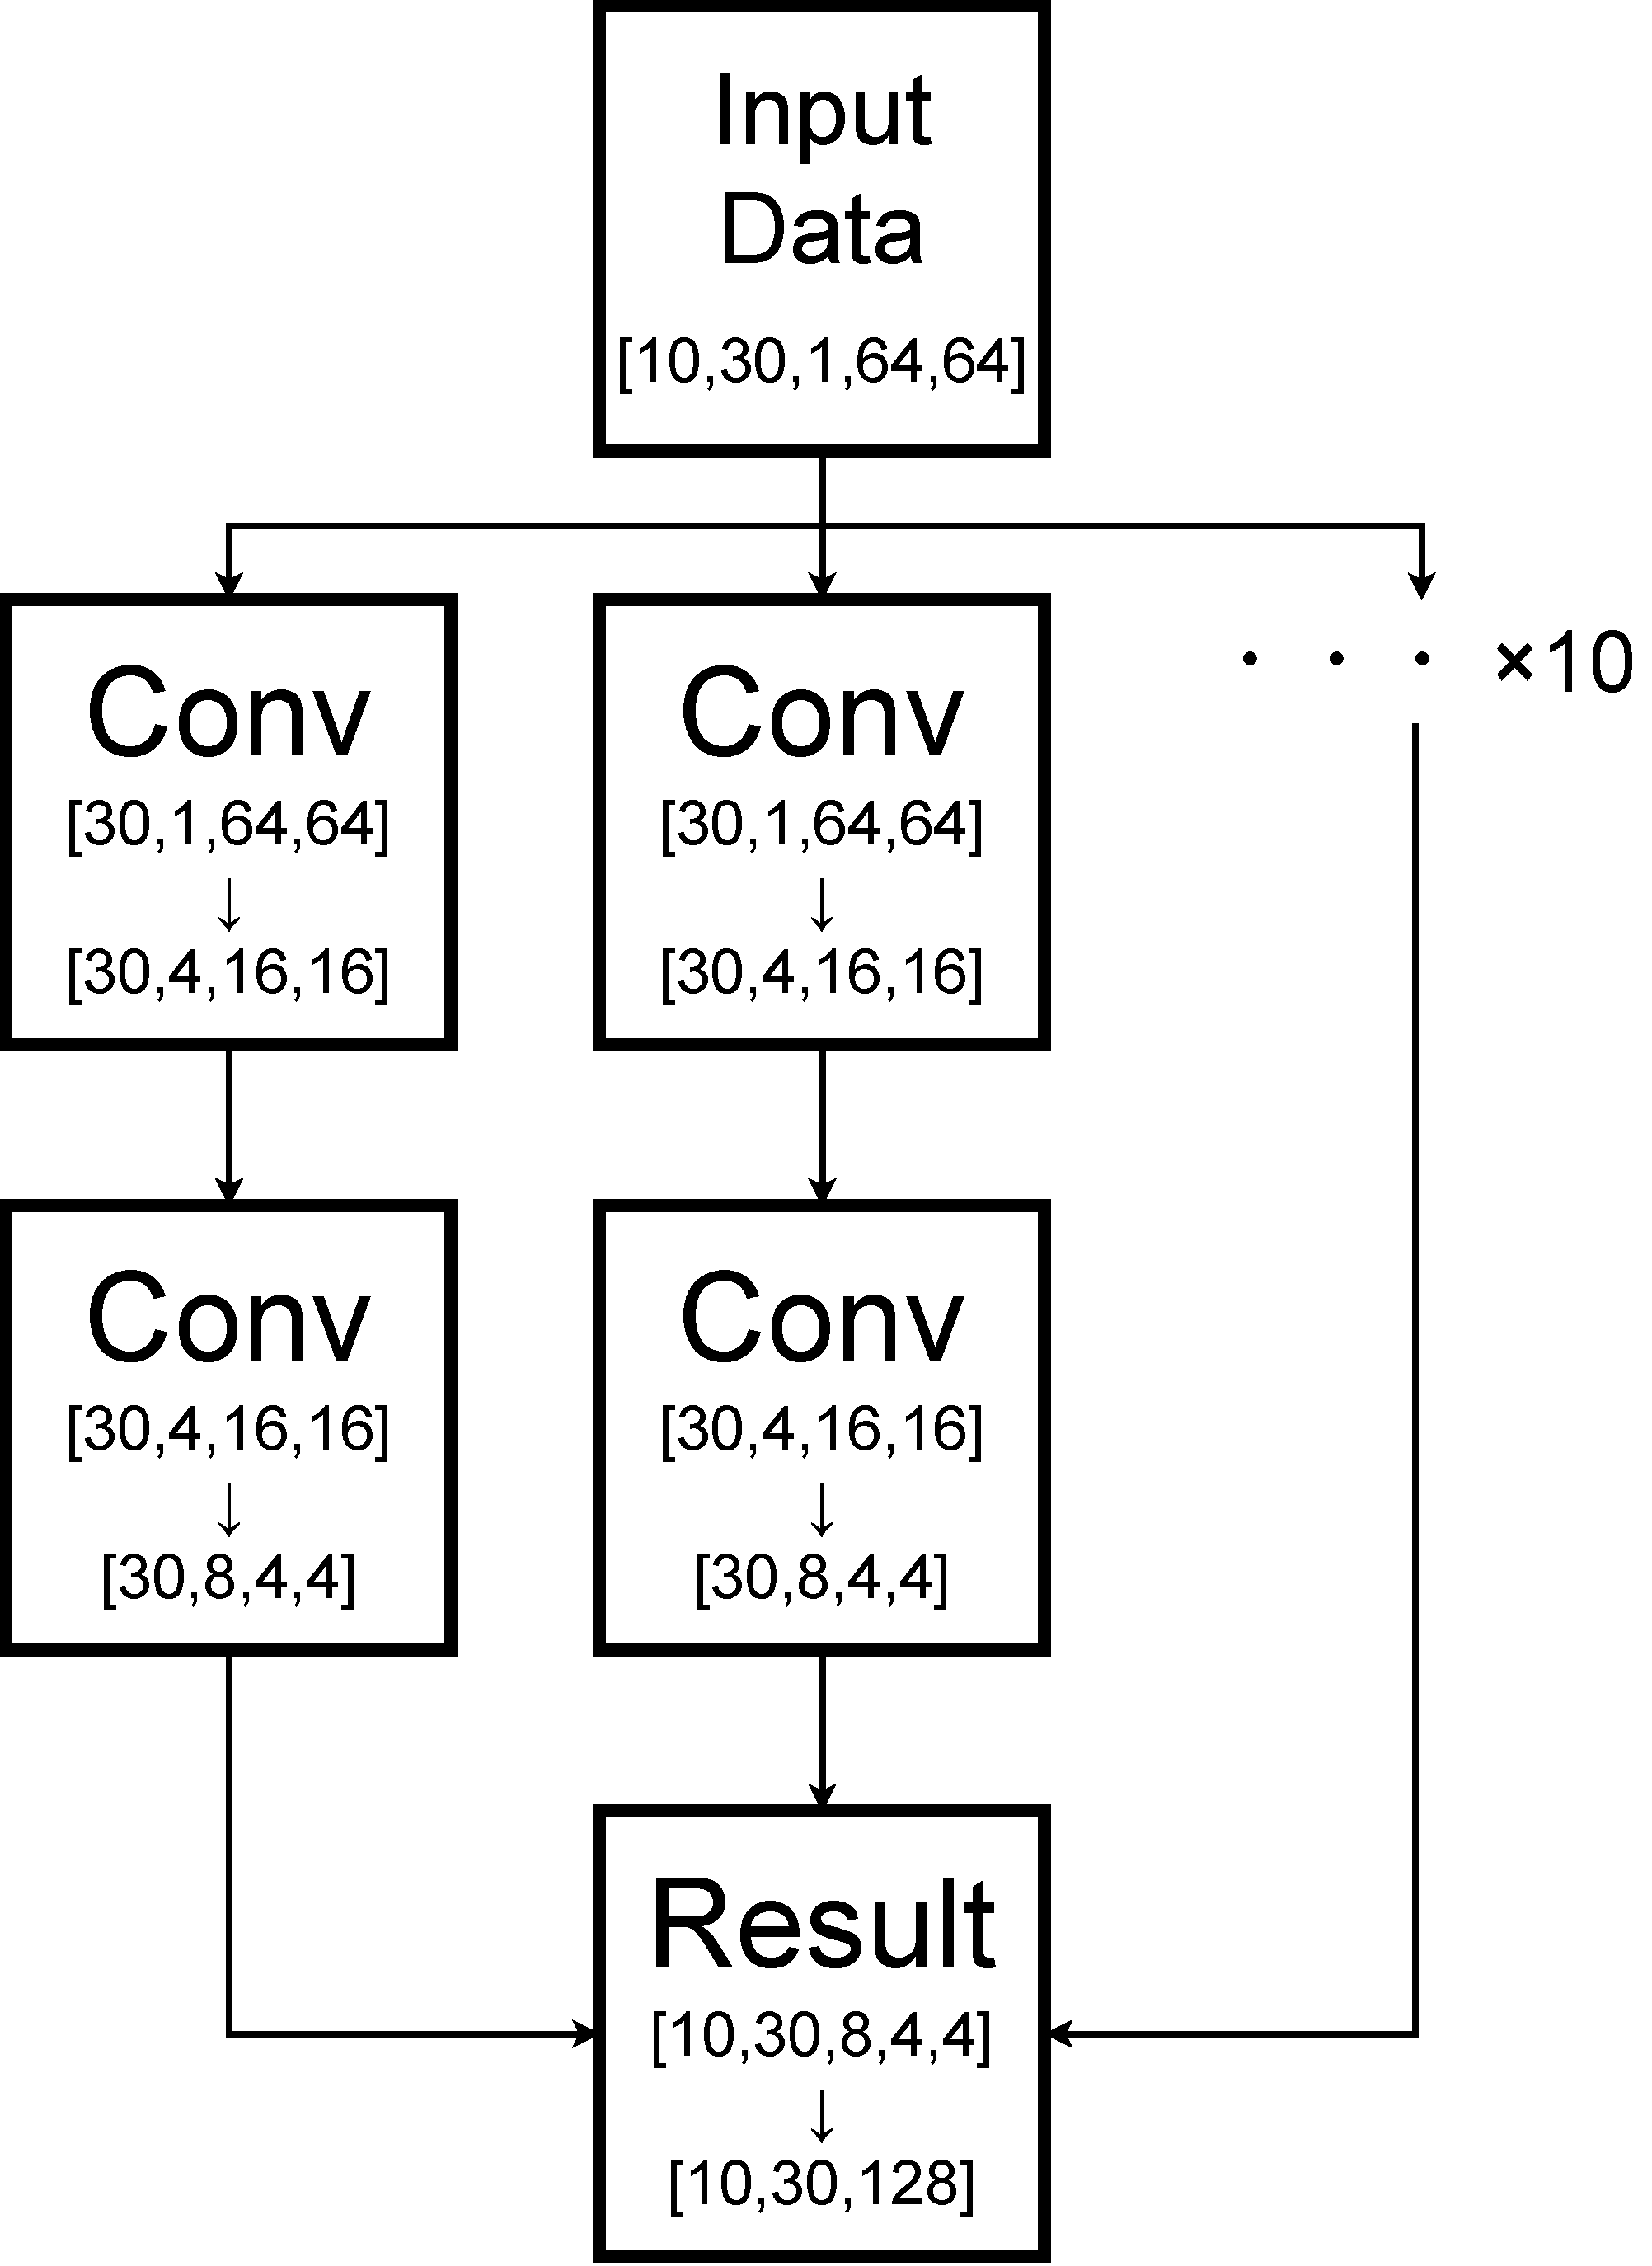
\includegraphics[width=80mm]{images/chart/conv.pdf}
  \end{center}
  \caption{畳み込み層}
  \label{conv}
\end{figure}

整形された動画データは図\ref{conv}のような畳み込み層を通過する.
入力データは[バッチ,フレーム長,画素数(グレースケールなので1),画像の縦データ,画像の横データ]の
5次元データである.これをそのまま処理しようとすると3次元の畳み込みを
使用する必要があり,動画像として処理したい今回にはそぐわない.
これを解決するために畳み込み層をバッチ数だけ存在させ,入力データをバッチ数だけ分割した.
これにより,[フレーム長,画素数(グレースケールなので1),画像の縦データ,画像の横データ]の
4次元データで処理させることができ,フレームをバッチに見立てることで
畳み込みの得意とする画像としての処理を実現させた.
\clearpage

\begin{figure}[t]
  \begin{center}
    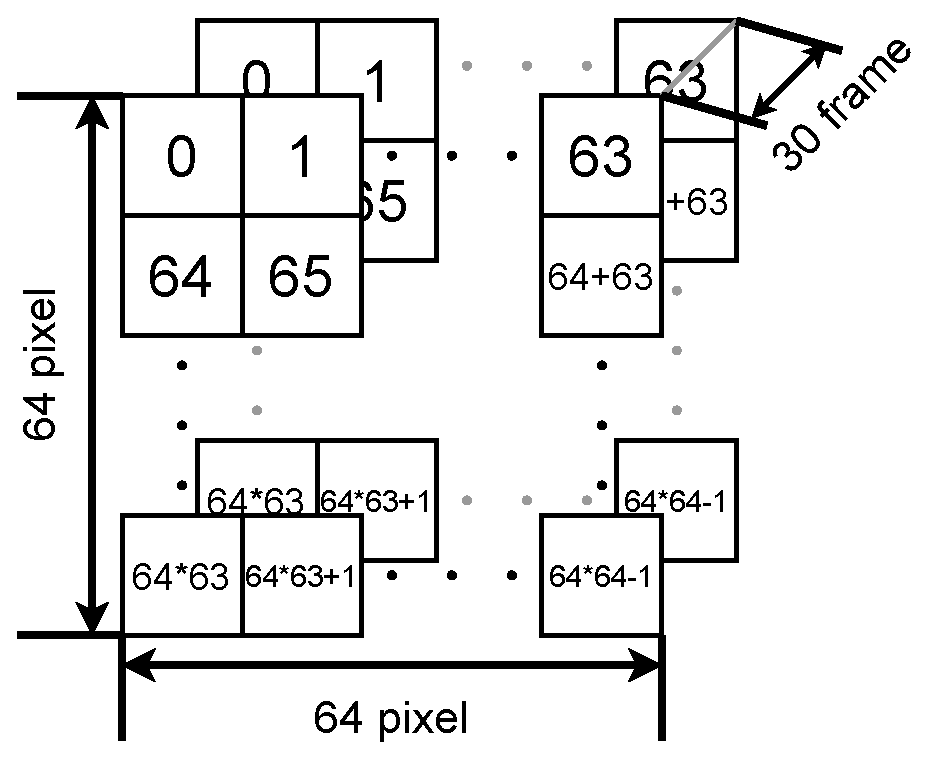
\includegraphics[width=120mm]{images/chart/embedding.pdf}
  \end{center}
  \caption{embeddingデータ}
  \label{embedding}
\end{figure}

次に図\ref{embedding}のようなピクセル情報を模した数値行列を同じ畳み込み層に通す.
この行列は64×64サイズに0から順にインデックス番号を持つ長さ指定フレーム長の行列である.
Transformerでは位置情報が喪失してしまうので位置情報を足し合わせることをする.
畳み込み後のデータは加工された動画データなのでインデックス番号を畳み込みすることで
同じ次元の位置情報を持たせることを試みた.
\clearpage

\begin{figure}[t]
  \begin{center}
    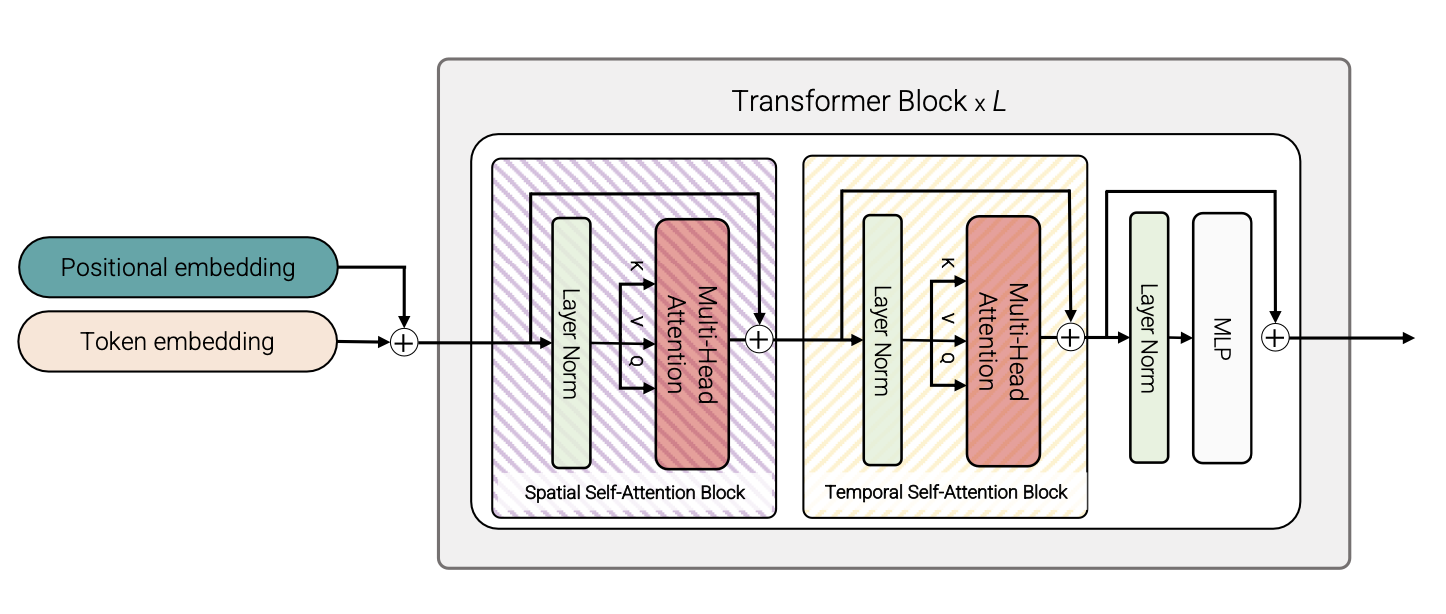
\includegraphics[width=130mm]{images/quote/encoder.png}
  \end{center}
  \caption{ViViTのEncoderモデル}
  \label{encoder}
\end{figure}

加工された動画データと位置情報を足し合わせ,Transformer Encoderに通す.
ヘッドを二つに分割したレイヤーを二つ重ね合わせた.
これもViViTに倣い図\ref{encoder}のような処理にした.実際,ヘッド数やレイヤー数は
これが最も精度良く推論できた.

最後に全結合層に通す.データを3に集約させるため,層を5つに分割し慎重に取り出した.
また,前半ではReLU(\ref{relu})活性化関数とすることでデータを減らし,
後半ではTanh(\ref{tanh})を活性化関数とすることでデータが影響し合えるようにした.

\begin{equation}
  \left\{
    \begin{array}{ll}
      f(x) = 0 & x \leq 0 \\
      f(x) = x & x > 0
    \end{array}
  \right.
  \label{relu}
\end{equation}

\begin{equation}
  f(x) = \frac{e^x - e^{-x}}{e^x + e^{-x}}
  \label{tanh}
\end{equation}

ネットワーク全体をフローチャートにすると図\ref{flowchart}のようになる.

\begin{figure}[b]
  \begin{center}
    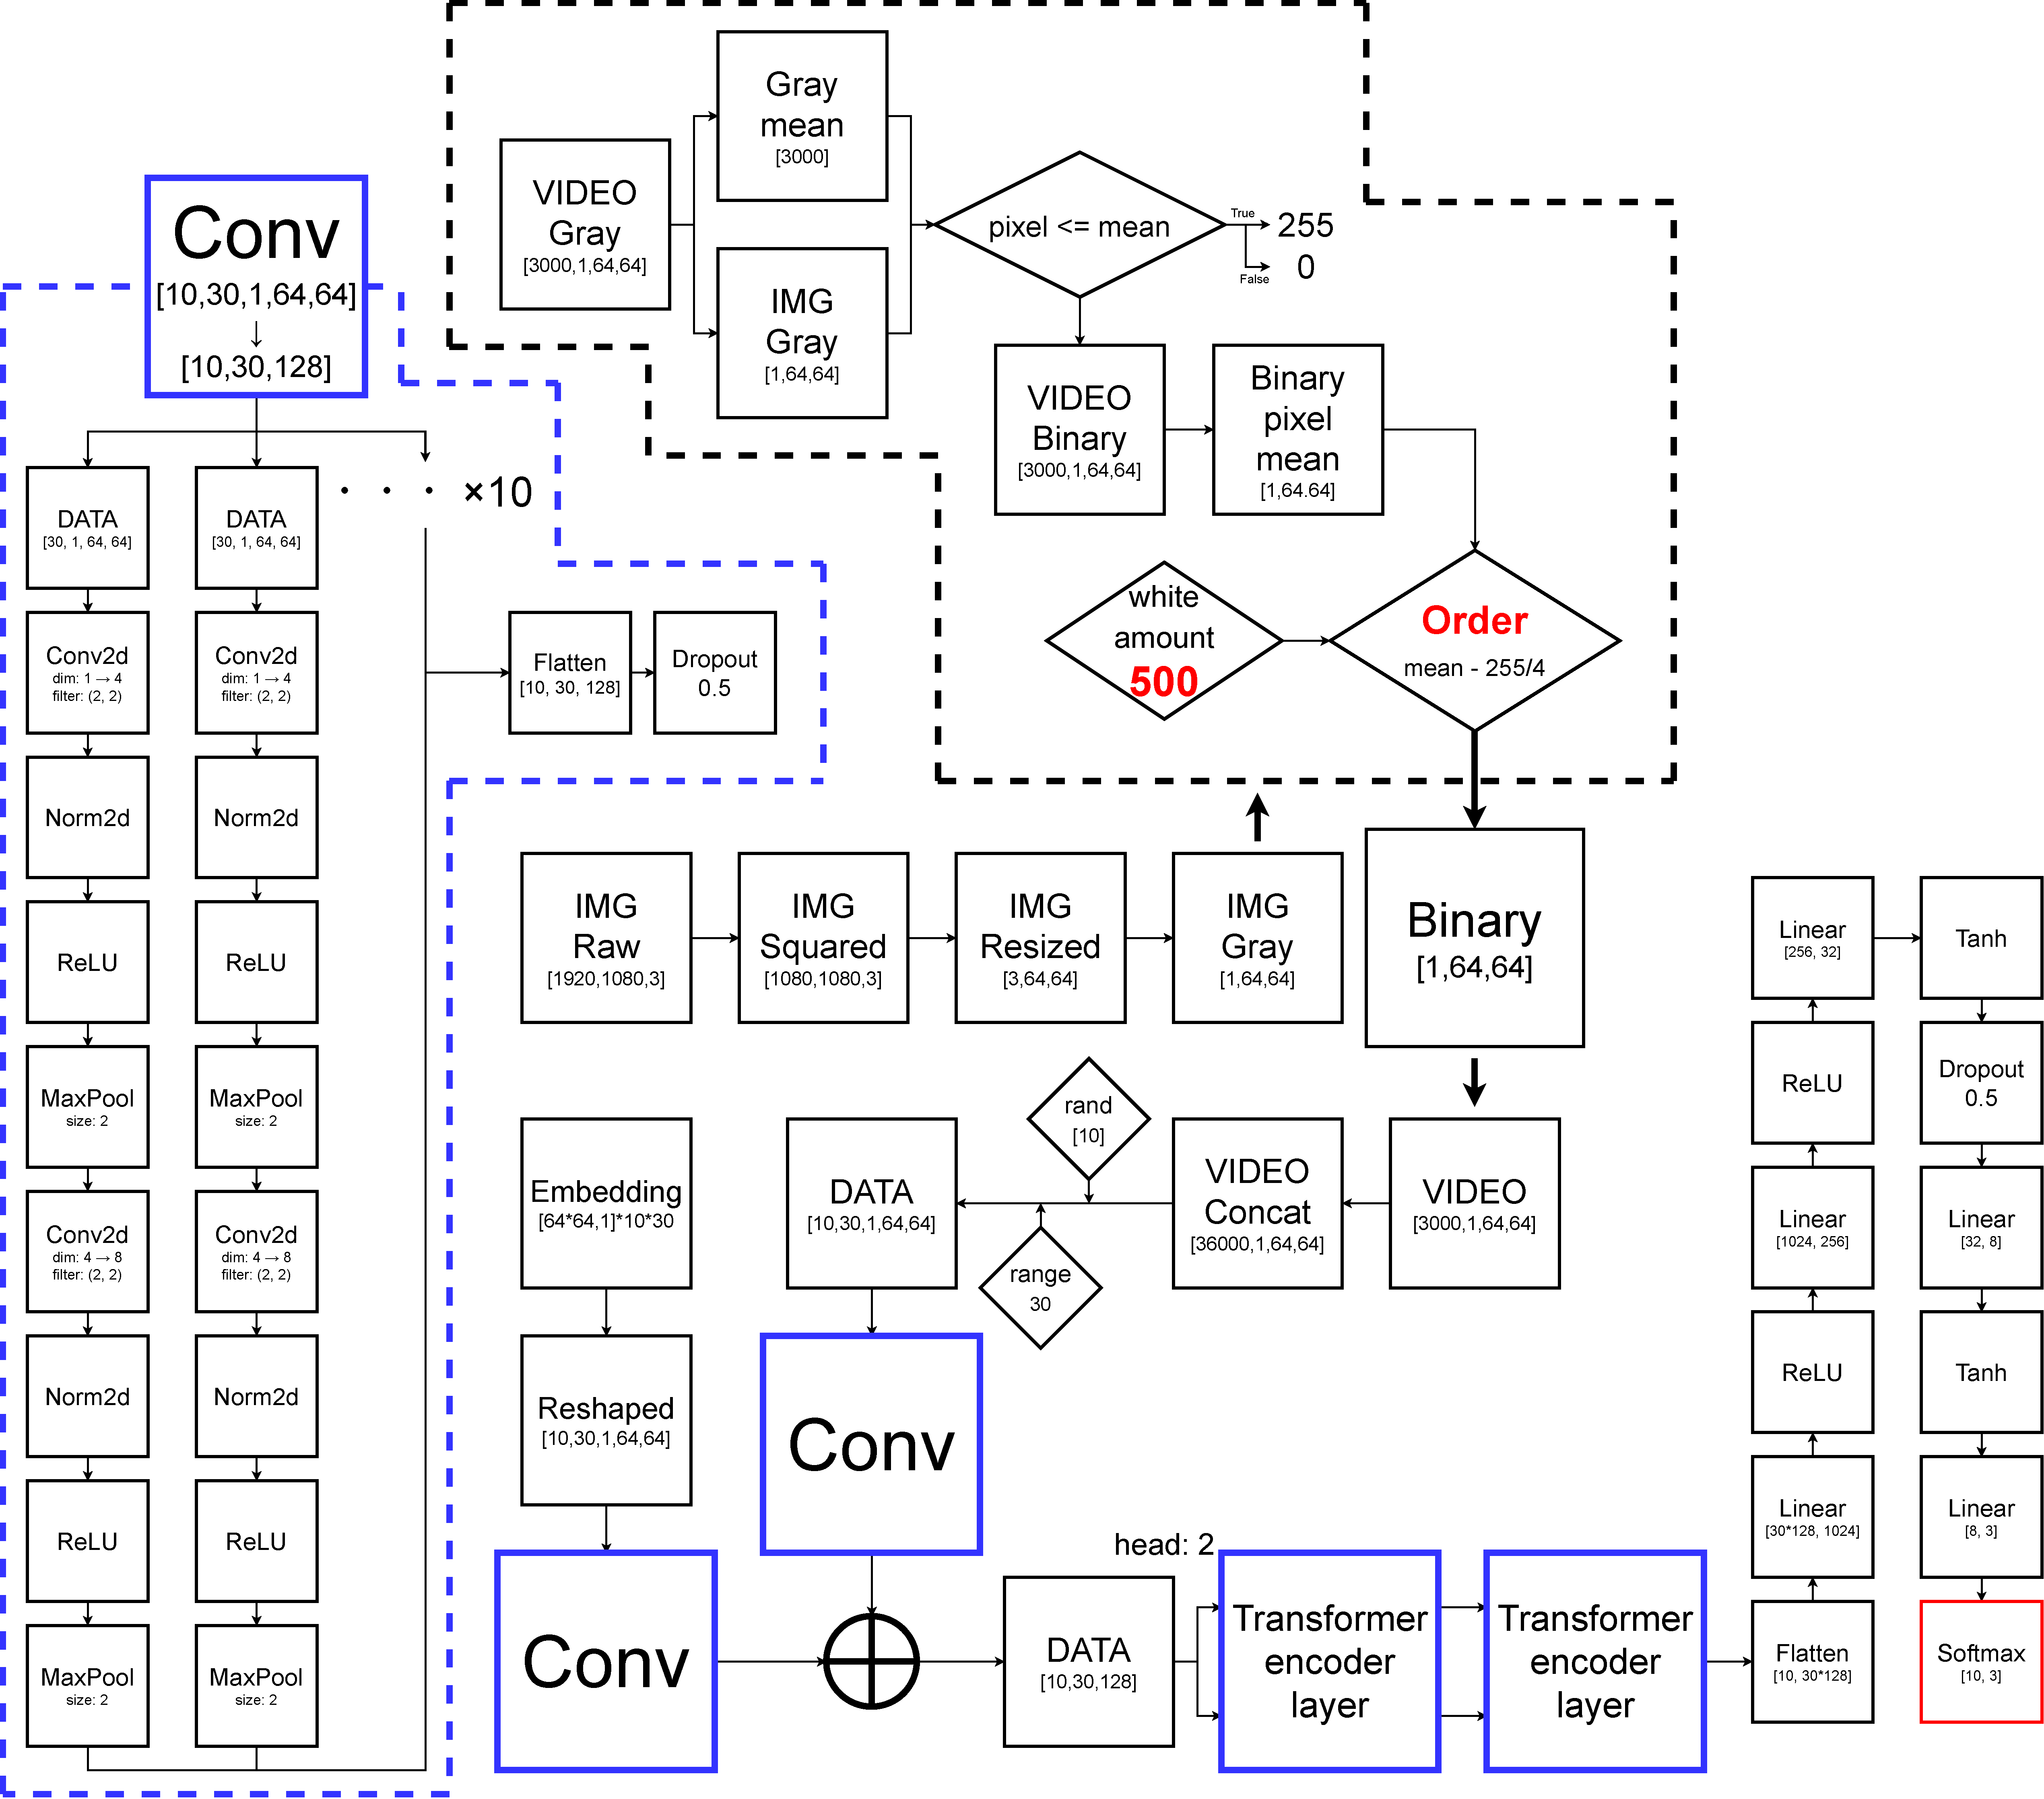
\includegraphics[width=130mm]{images/chart/flowchart.pdf}
  \end{center}
  \caption{ネットワーク全体}
  \label{flowchart}
\end{figure}
\clearpage

\subsection{精度}
作成したネットワークが学習できているか確認するために,動画数を変化させて
その精度の推移を確認した.
表\ref{result}のように動画を3つずつ増やした結果,精度が向上していることがわかった.

\begin{table}[b]
  \begin{center}
    \begin{tabular}{|c|} \hline
      結果と使用動画 \\ \hline
        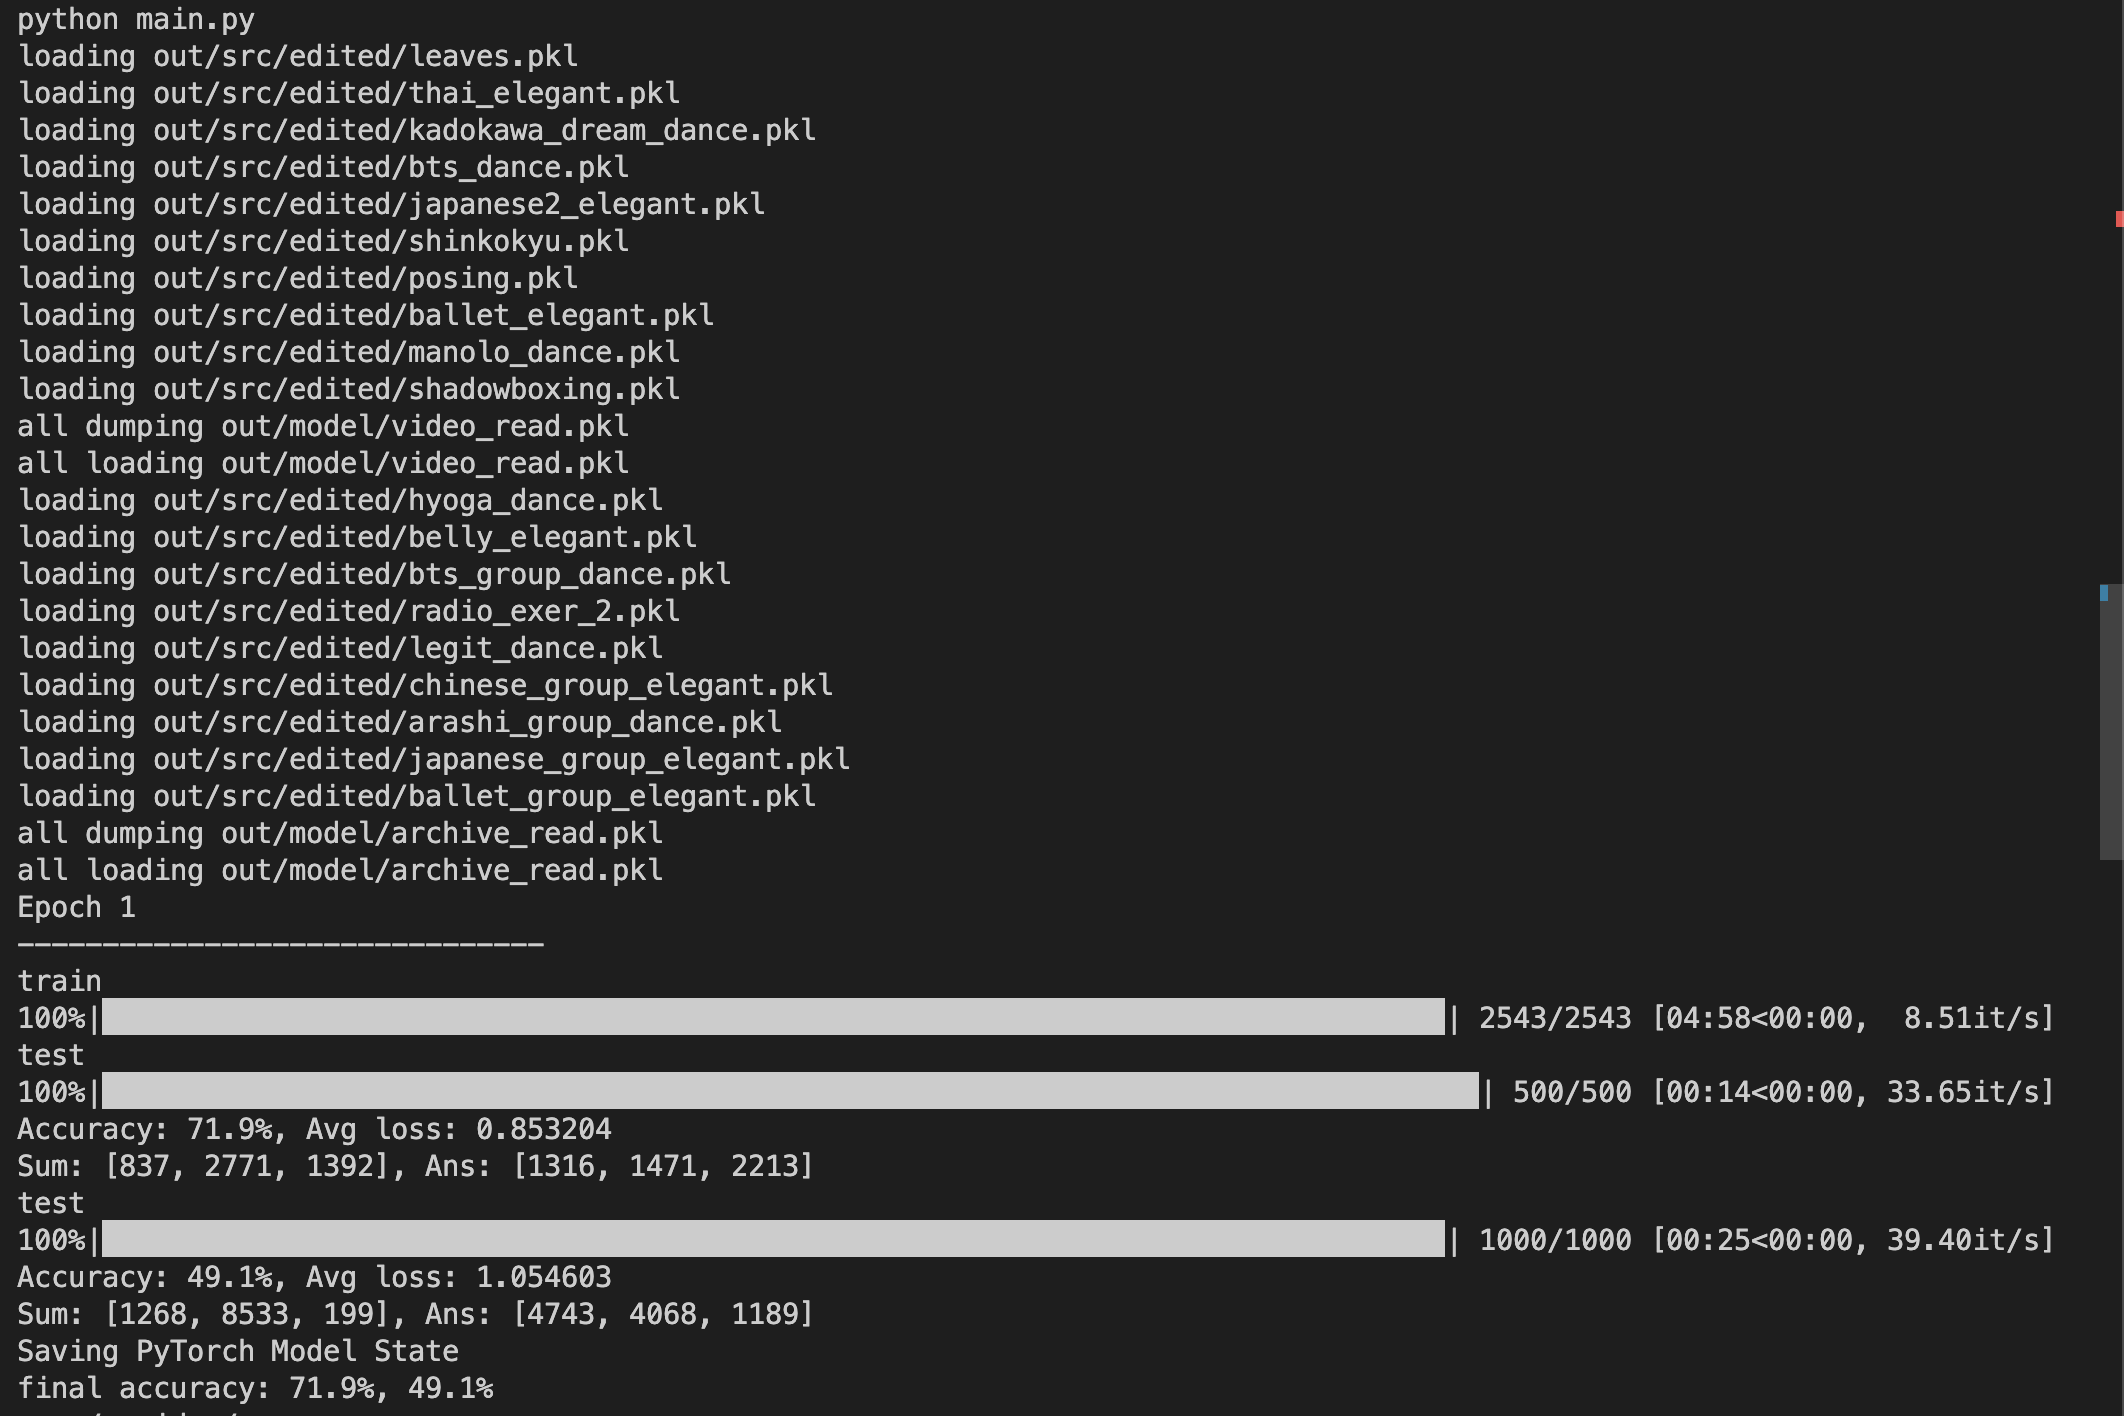
\includegraphics[width=110mm]{images/net_result/result10.png}
      \\
        \cite{ballet}\cite{thai}\cite{jpn2}
        \cite{kadokawa}\cite{bts}\cite{manolo}
        \cite{posing}\cite{boxing}\cite{shinkokyu}\cite{leaves}
      \\ \hline
        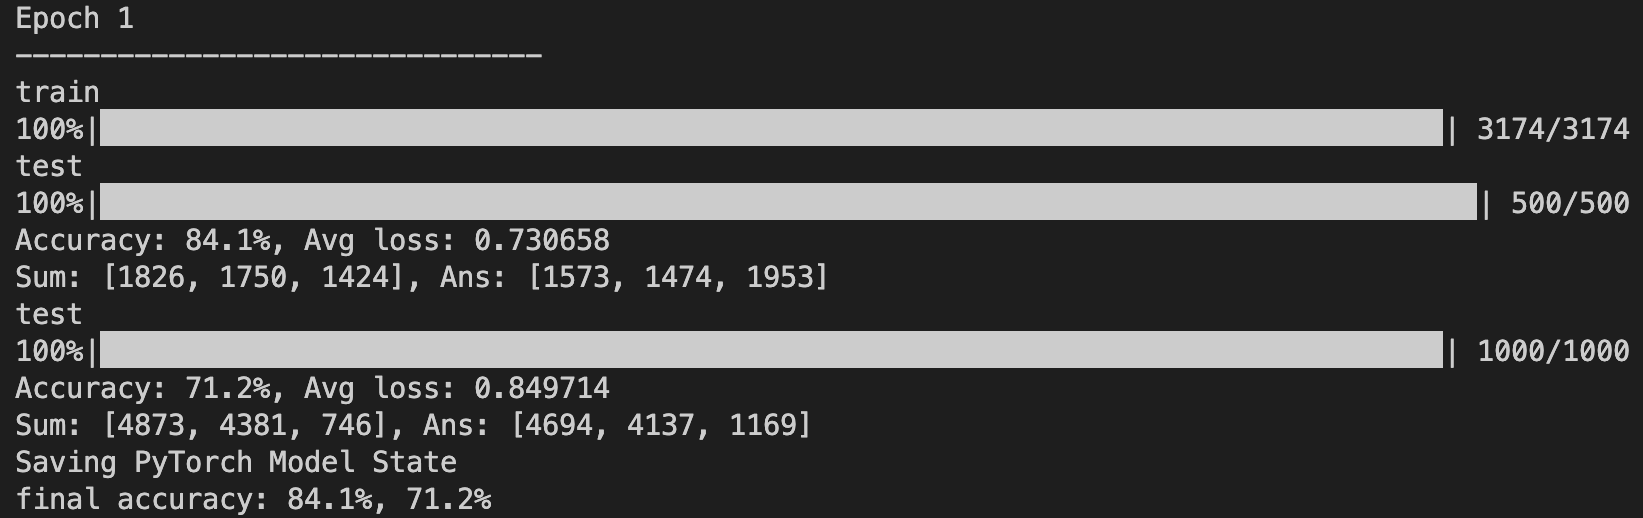
\includegraphics[width=110mm]{images/net_result/result13.png}
      \\
        \cite{jpn}\cite{ballet}\cite{thai}\cite{jpn2}
        \cite{ariana}\cite{kadokawa}\cite{bts}\cite{manolo}
        \cite{posing}\cite{boxing}\cite{running}\cite{shinkokyu}\cite{leaves}
      \\ \hline
        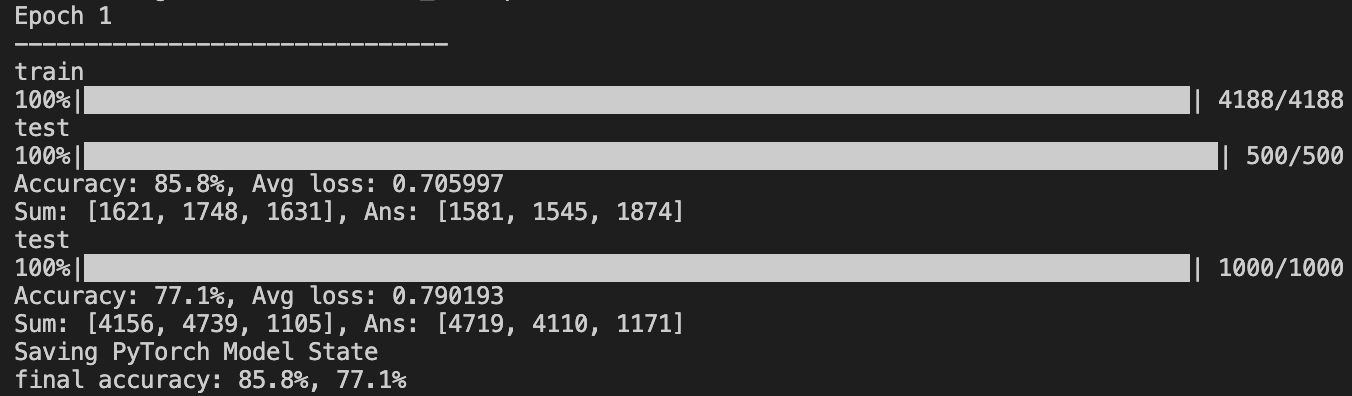
\includegraphics[width=110mm]{images/net_result/result16.png}
      \\
        \cite{jpn}\cite{china}\cite{ballet}\cite{thai}\cite{jpn2}
        \cite{ariana}\cite{kadokawa}\cite{bts}\cite{manolo}\cite{aito}
        \cite{radio}\cite{posing}\cite{boxing}\cite{running}\cite{shinkokyu}\cite{leaves}
      \\ \hline
    \end{tabular}
  \end{center}
  \caption{使用動画別の精度}
  \label{result}
\end{table}
\clearpage

次にバッチサイズ別に精度の推移を確認した.
表\ref{batch}のようにバッチが少ないほど学習,推論共に精度が高いことが確認された.
一般にバッチは処理時間の短縮のために使われる.1回に処理するデータが少ない方が精度は
高くなるが,その分用意したデータを全て学習するのに時間がかかる.
また,3章で使用するGrad Camでは判断根拠可視化のために大量のデータを必要とするので
バッチ数が少ないとその特徴がほとんど現れないことを確認している.
よって3章ではバッチ数10を使用することとした.

\begin{table}[b]
  \begin{center}
    \begin{tabular}{|c|} \hline
      結果とバッチサイズ \\ \hline
        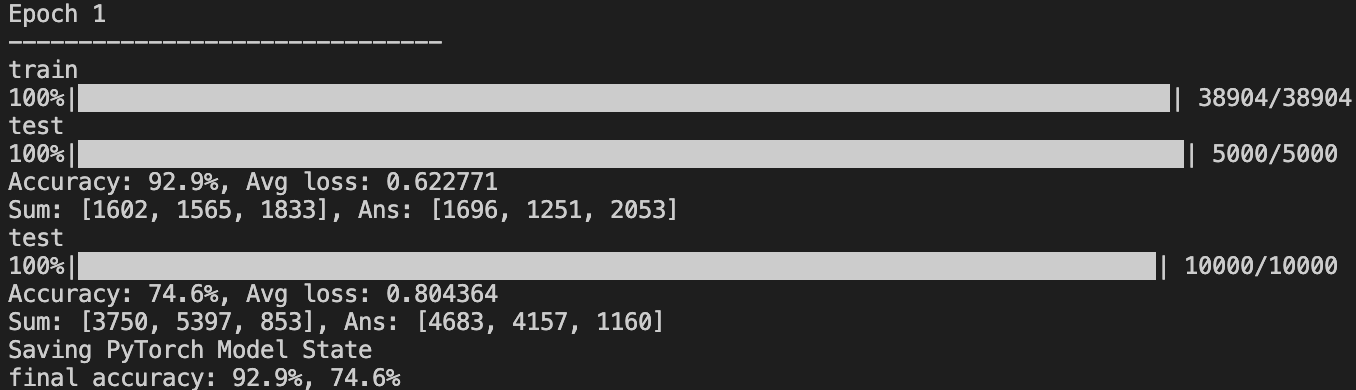
\includegraphics[width=110mm]{images/net_result/batch1.png} \\ batch:1 \\ \hline
        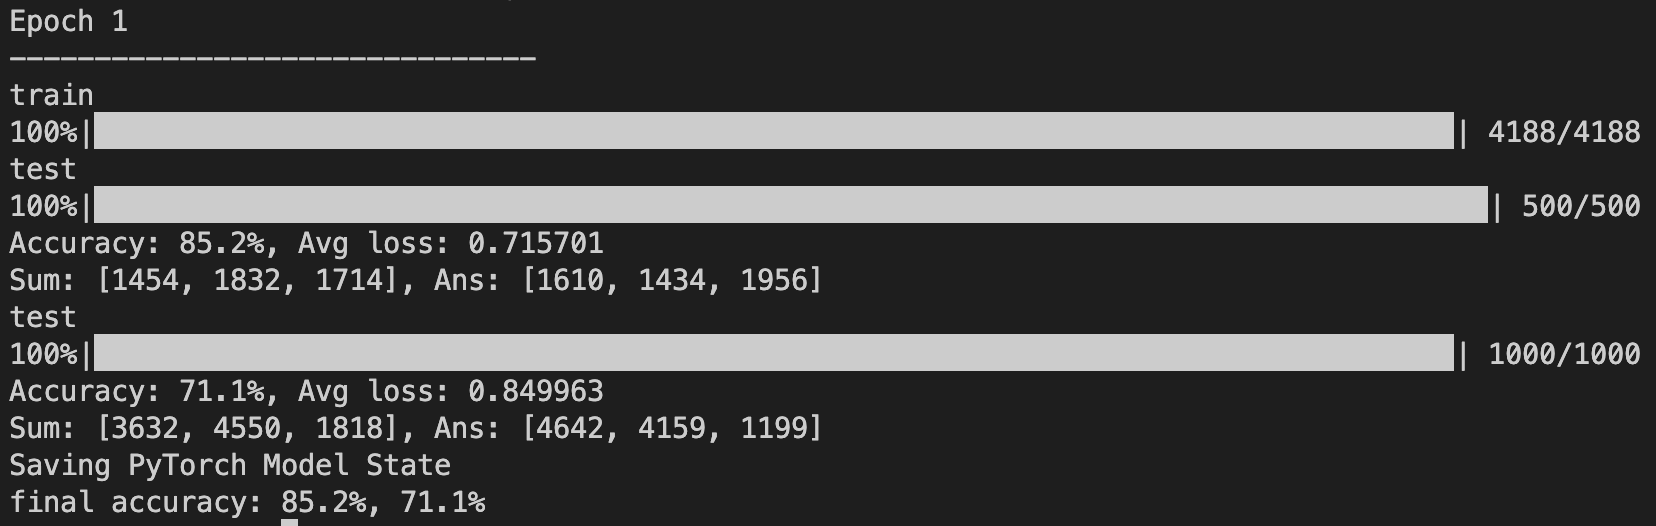
\includegraphics[width=110mm]{images/net_result/batch10.png} \\ batch:10 \\ \hline
        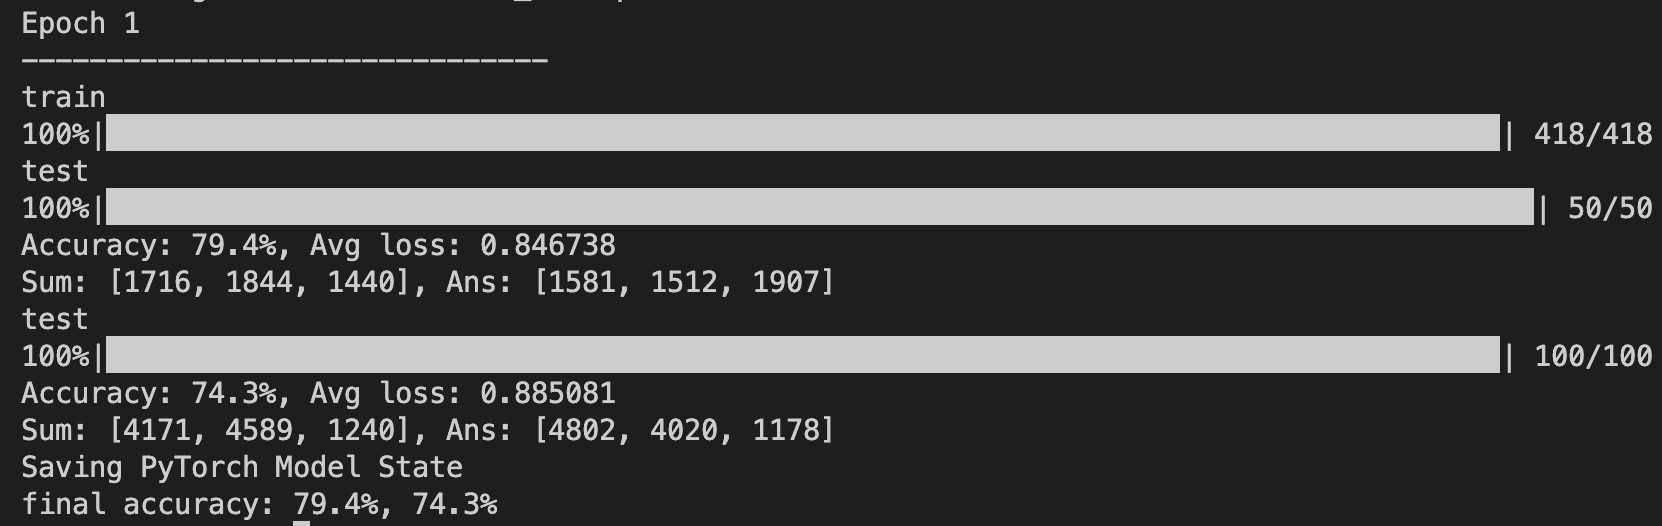
\includegraphics[width=110mm]{images/net_result/batch100.png} \\ batch:100 \\ \hline
    \end{tabular}
  \end{center}
  \caption{batch別の精度}
  \label{batch}
\end{table}
\clearpage

次に学習,エポック毎で損失がどのように推移するか確認した.エポックとは,同一のデータを
繰り返し学習させることである.
表\ref{epoch}のように1回目のエポックでほとんど収束して行き,エポックを重ねるごとに
その値の揺れが小さくなっていることが分かった.

これらのことから制作したネットワークが正常に学習を進めていることが分かった.
また,学習データに対して8割程度の精度であったとしても,推論時も7.5割程度で
判別することができることが分かった.

\begin{table}[b]
  \begin{center}
    \begin{tabular}{|c|} \hline
      結果とエポック数 \\ \hline
        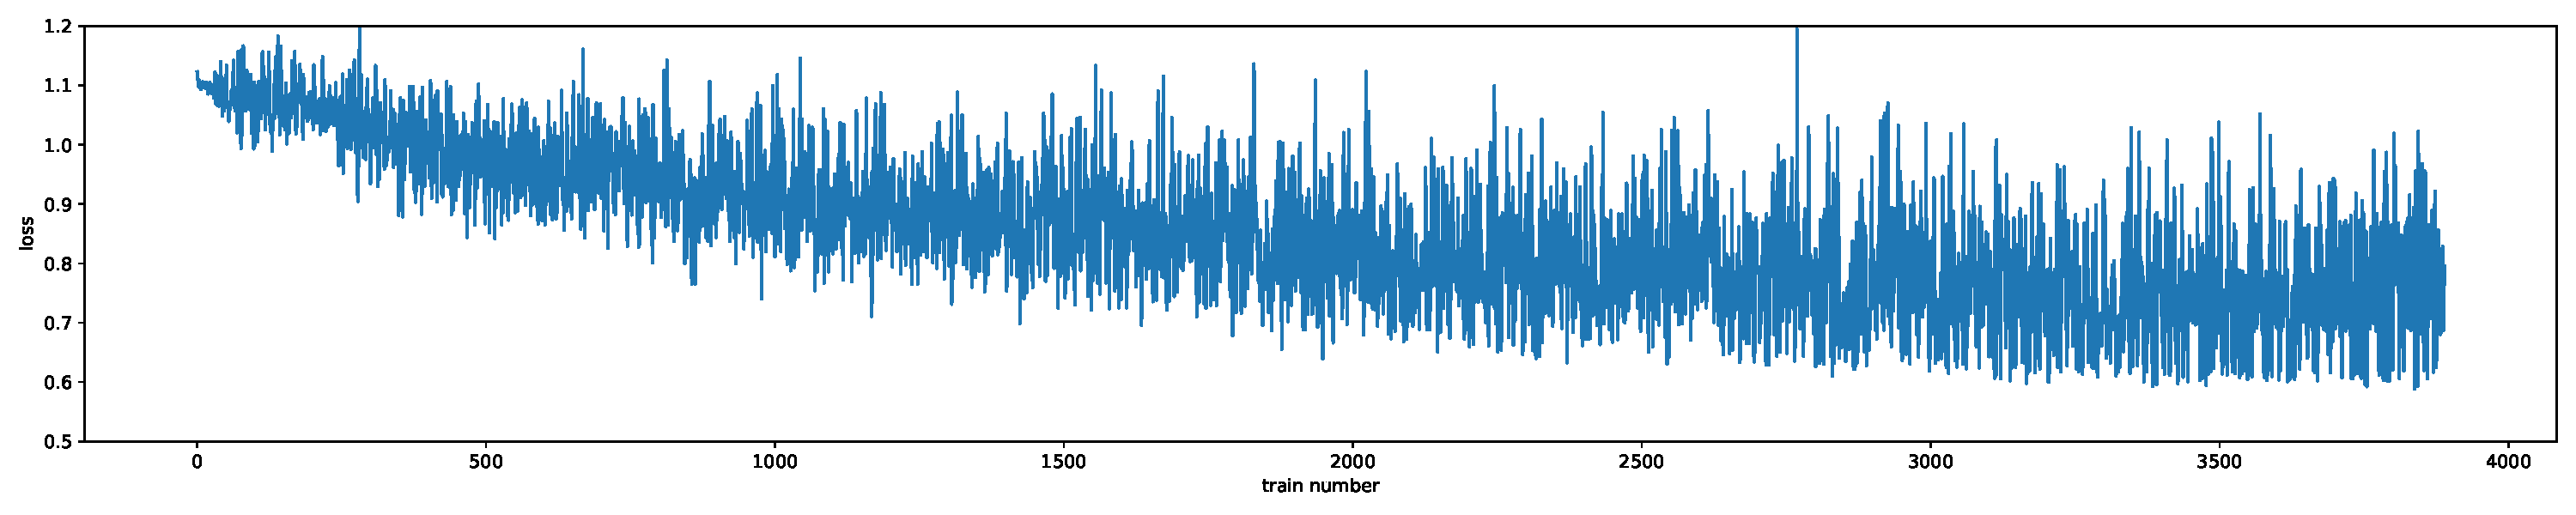
\includegraphics[width=130mm]{images/net_result/epoch_1.pdf} \\ epoch:1 \\ \hline
        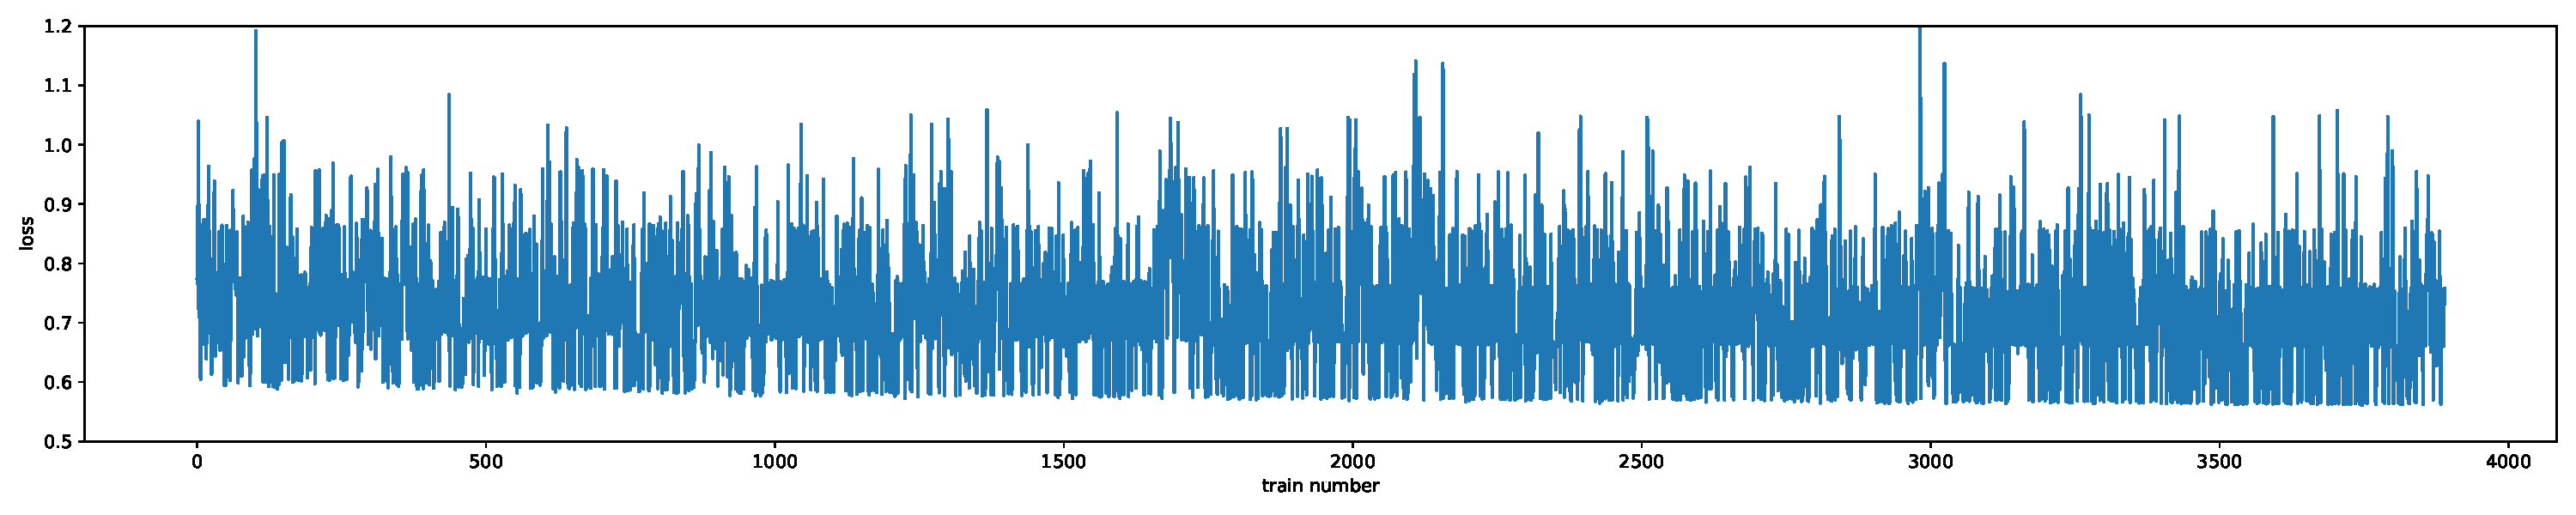
\includegraphics[width=130mm]{images/net_result/epoch_2.pdf} \\ epoch:2 \\ \hline
        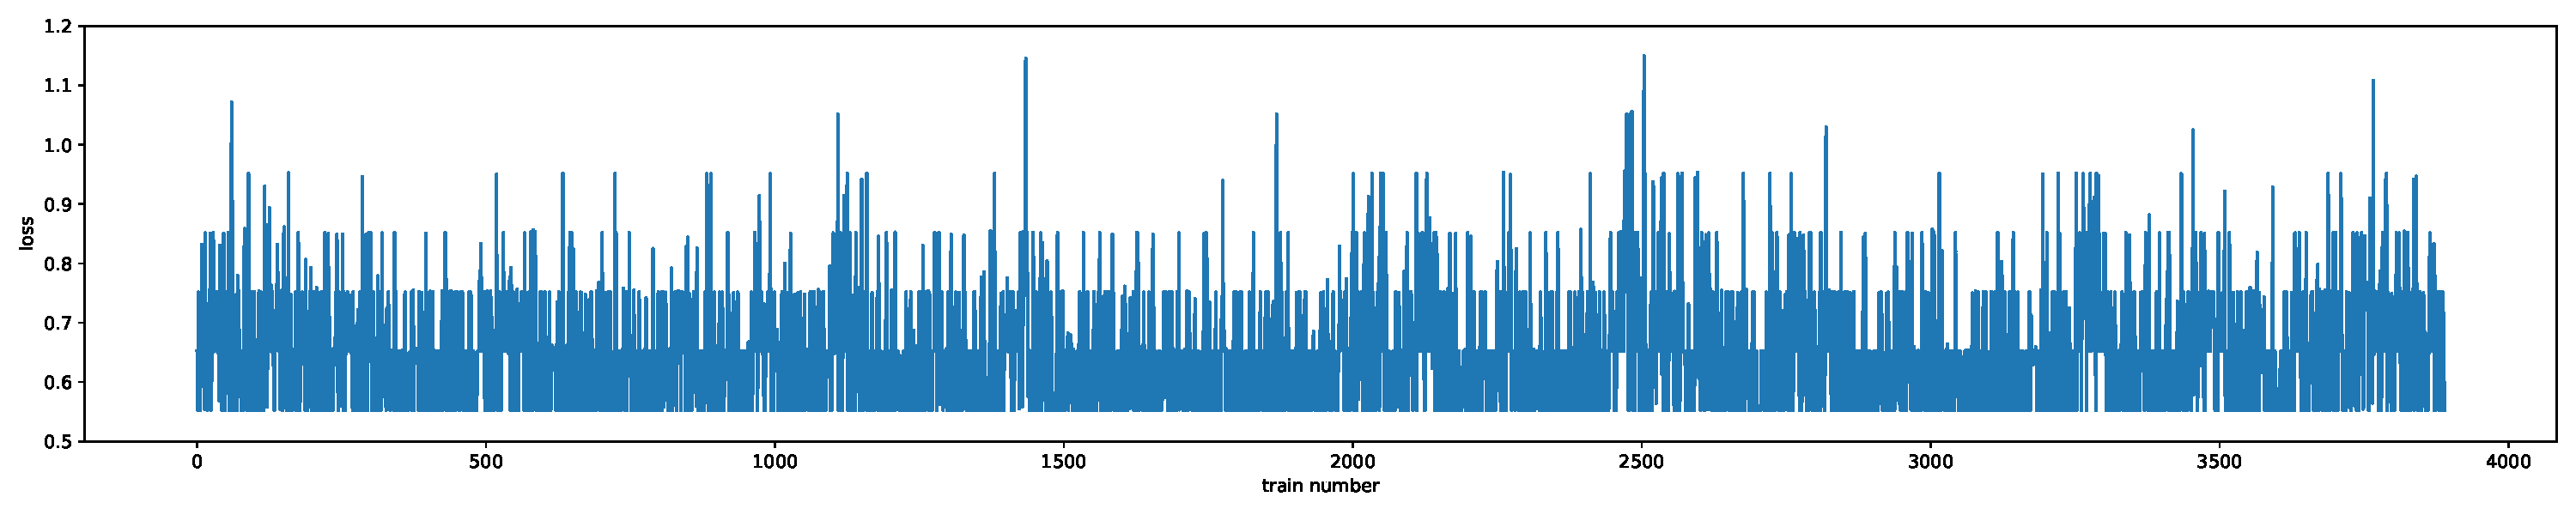
\includegraphics[width=130mm]{images/net_result/epoch_10.pdf} \\ epoch:10 \\ \hline
    \end{tabular}
  \end{center}
  \caption{epoch毎の損失推移}
  \label{epoch}
\end{table}
\clearpage